
%% bare_jrnl_compsoc.tex
%% V1.4b
%% 2015/08/26
%% by Michael Shell
%% See:
%% http://www.michaelshell.org/
%% for current contact information.
%%
%% This is a skeleton file demonstrating the use of IEEEtran.cls
%% (requires IEEEtran.cls version 1.8b or later) with an IEEE
%% Computer Society journal paper.
%%
%% Support sites:
%% http://www.michaelshell.org/tex/ieeetran/
%% http://www.ctan.org/pkg/ieeetran
%% and
%% http://www.ieee.org/

%%*************************************************************************
%% Legal Notice:
%% This code is offered as-is without any warranty either expressed or
%% implied; without even the implied warranty of MERCHANTABILITY or
%% FITNESS FOR A PARTICULAR PURPOSE! 
%% User assumes all risk.
%% In no event shall the IEEE or any contributor to this code be liable for
%% any damages or losses, including, but not limited to, incidental,
%% consequential, or any other damages, resulting from the use or misuse
%% of any information contained here.
%%
%% All comments are the opinions of their respective authors and are not
%% necessarily endorsed by the IEEE.
%%
%% This work is distributed under the LaTeX Project Public License (LPPL)
%% ( http://www.latex-project.org/ ) version 1.3, and may be freely used,
%% distributed and modified. A copy of the LPPL, version 1.3, is included
%% in the base LaTeX documentation of all distributions of LaTeX released
%% 2003/12/01 or later.
%% Retain all contribution notices and credits.
%% ** Modified files should be clearly indicated as such, including  **
%% ** renaming them and changing author support contact information. **
%%*************************************************************************


% *** Authors should verify (and, if needed, correct) their LaTeX system  ***
% *** with the testflow diagnostic prior to trusting their LaTeX platform ***
% *** with production work. The IEEE's font choices and paper sizes can   ***
% *** trigger bugs that do not appear when using other class files.       ***                          ***
% The testflow support page is at:
% http://www.michaelshell.org/tex/testflow/


\documentclass[10pt,journal,compsoc]{IEEEtran}

%
% If IEEEtran.cls has not been installed into the LaTeX system files,
% manually specify the path to it like:
% \documentclass[10pt,journal,compsoc]{../sty/IEEEtran}





% Some very useful LaTeX packages include:
% (uncomment the ones you want to load)


% *** MISC UTILITY PACKAGES ***
%
\usepackage{ifpdf}
% Heiko Oberdiek's ifpdf.sty is very useful if you need conditional
% compilation based on whether the output is pdf or dvi.
% usage:
% \ifpdf
%   % pdf code
% \else
%   % dvi code
% \fi
% The latest version of ifpdf.sty can be obtained from:
% http://www.ctan.org/pkg/ifpdf
% Also, note that IEEEtran.cls V1.7 and later provides a builtin
% \ifCLASSINFOpdf conditional that works the same way.
% When switching from latex to pdflatex and vice-versa, the compiler may
% have to be run twice to clear warning/error messages.






% *** CITATION PACKAGES ***
%
\ifCLASSOPTIONcompsoc
  % IEEE Computer Society needs nocompress option
  % requires cite.sty v4.0 or later (November 2003)
  \usepackage[nocompress]{cite}
\else
  % normal IEEE
  \usepackage{cite}
\fi
% cite.sty was written by Donald Arseneau
% V1.6 and later of IEEEtran pre-defines the format of the cite.sty package
% \cite{} output to follow that of the IEEE. Loading the cite package will
% result in citation numbers being automatically sorted and properly
% "compressed/ranged". e.g., [1], [9], [2], [7], [5], [6] without using
% cite.sty will become [1], [2], [5]--[7], [9] using cite.sty. cite.sty's
% \cite will automatically add leading space, if needed. Use cite.sty's
% noadjust option (cite.sty V3.8 and later) if you want to turn this off
% such as if a citation ever needs to be enclosed in parenthesis.
% cite.sty is already installed on most LaTeX systems. Be sure and use
% version 5.0 (2009-03-20) and later if using hyperref.sty.
% The latest version can be obtained at:
% http://www.ctan.org/pkg/cite
% The documentation is contained in the cite.sty file itself.
%
% Note that some packages require special options to format as the Computer
% Society requires. In particular, Computer Society  papers do not use
% compressed citation ranges as is done in typical IEEE papers
% (e.g., [1]-[4]). Instead, they list every citation separately in order
% (e.g., [1], [2], [3], [4]). To get the latter we need to load the cite
% package with the nocompress option which is supported by cite.sty v4.0
% and later. Note also the use of a CLASSOPTION conditional provided by
% IEEEtran.cls V1.7 and later.





% *** GRAPHICS RELATED PACKAGES ***
%
\ifCLASSINFOpdf
   \usepackage[pdftex]{graphicx}
   \graphicspath{{figures/}{pictures/}{images/}{./}}
  % declare the path(s) where your graphic files are
  % \graphicspath{{../pdf/}{../jpeg/}}
  % and their extensions so you won't have to specify these with
  % every instance of \includegraphics
   \DeclareGraphicsExtensions{.pdf,.jpeg,.png}
\else
  % or other class option (dvipsone, dvipdf, if not using dvips). graphicx
  % will default to the driver specified in the system graphics.cfg if no
  % driver is specified.
   \usepackage[dvips]{graphicx}
   \graphicspath{{figures/}{pictures/}{images/}{./}}
  % declare the path(s) where your graphic files are
  % \graphicspath{{../eps/}}
  % and their extensions so you won't have to specify these with
  % every instance of \includegraphics
   \DeclareGraphicsExtensions{.eps}
\fi
% graphicx was written by David Carlisle and Sebastian Rahtz. It is
% required if you want graphics, photos, etc. graphicx.sty is already
% installed on most LaTeX systems. The latest version and documentation
% can be obtained at: 
% http://www.ctan.org/pkg/graphicx
% Another good source of documentation is "Using Imported Graphics in
% LaTeX2e" by Keith Reckdahl which can be found at:
% http://www.ctan.org/pkg/epslatex
%
% latex, and pdflatex in dvi mode, support graphics in encapsulated
% postscript (.eps) format. pdflatex in pdf mode supports graphics
% in .pdf, .jpeg, .png and .mps (metapost) formats. Users should ensure
% that all non-photo figures use a vector format (.eps, .pdf, .mps) and
% not a bitmapped formats (.jpeg, .png). The IEEE frowns on bitmapped formats
% which can result in "jaggedy"/blurry rendering of lines and letters as
% well as large increases in file sizes.
%
% You can find documentation about the pdfTeX application at:
% http://www.tug.org/applications/pdftex

\usepackage{microtype}                 % use micro-typography (slightly more compact, better to read)
\PassOptionsToPackage{warn}{textcomp}  % to address font issues with \textrightarrow
%\usepackage{textcomp}                  % use better special symbols
%\usepackage{mathptmx}                  % use matching math font
%\usepackage{times}                     % we use Times as the main font
%\renewcommand*\ttdefault{txtt}         % a nicer typewriter font
\usepackage{cite}                      % needed to automatically sort the references
\usepackage{tabu}                      % only used for the table example
\usepackage{booktabs}                  % only used for the table example


\usepackage{tabularx,ragged2e,booktabs}
\usepackage{bm}
\usepackage{enumerate}
\usepackage{indentfirst}
\usepackage{multirow} 
\usepackage{rotating} 
\usepackage{booktabs} 
\usepackage{setspace} 
\usepackage{color}   
\usepackage{verbatim}
% \usepackage[fleqn]{amsmath}
\usepackage{amsmath}


% additional packages
% \usepackage{float}
\usepackage{hyperref}
\usepackage{amssymb}
\usepackage{amsfonts}
% \usepackage{subfig}
\usepackage{floatrow}
\floatsetup[table]{capposition=top}
\usepackage{bm} % for bold for vector
\usepackage[locale=FR]{siunitx} % for micro sec
% \usepackage{helvet}
\usepackage[font=footnotesize,labelfont=sf,textfont=sf]{caption}
\usepackage{paralist} % for compactitem
%\captionsetup[subfloat]{font=footnotesize,labelfont=sf,textfont=sf,captionskip=5pt}

%\setlength\abovecaptionskip{5pt}
%\floatsetup{captionskip=5pt}
% \usepackage{floatrow}
% \floatsetup{captionskip=3pt}
%\setlength{\textfloatsep}{6pt plus 1.0pt minus 2.0pt}
%\setlength{\floatsep}{4pt plus 1.0pt minus 2.0pt}
%\setlength{\dbltextfloatsep}{6pt plus 2.0pt minus 0.0pt}
%\setlength{\dblfloatsep}{4pt plus 2.0pt minus 0.0pt}

\usepackage{algorithm}
\usepackage{algpseudocode}
\usepackage[locale=FR]{siunitx} % for units

\usepackage{scalerel} % inline figure
\usepackage{ragged2e}


% for autoref
\renewcommand{\sectionautorefname}{Sec.}
\renewcommand{\subsectionautorefname}{\sectionautorefname}
\renewcommand{\subsubsectionautorefname}{\sectionautorefname}
\renewcommand{\figureautorefname}{Fig.}
% \newcommand{\subfigureautorefname}{\figureautorefname}
\renewcommand{\tableautorefname}{Tab.}
\newcommand{\algorithmautorefname}{Algo.}
\renewcommand{\equationautorefname}{Eq.}



\usepackage{xcolor}
\newcommand{\TF}{\textcolor{red}}

%\newcommand{\clc}[1]{#1}
\newcommand{\clc}[1]{\smash{\raisebox{-0.4ex}{\scaleto{\includegraphics{images/icons/coloredCircle_#1.png}}{9px}}}}

% \newcommand{\glf}[1]{#1}
\newcommand{\glf}[1]{\smash{\raisebox{-0.4ex}{\scaleto{\includegraphics{images/icons/blackCircle_#1.pdf}}{9px}}}}

% \newcommand{\glfw}[1]{#1}
\newcommand{\glfw}[1]{\smash{\raisebox{-0.4ex}{\scaleto{\includegraphics{images/icons/whiteCircle_#1.pdf}}{9px}}}}

\newcommand{\circled}[1]{#1}



% *** MATH PACKAGES ***
%
\usepackage{amsmath}
% A popular package from the American Mathematical Society that provides
% many useful and powerful commands for dealing with mathematics.
%
% Note that the amsmath package sets \interdisplaylinepenalty to 10000
% thus preventing page breaks from occurring within multiline equations. Use:
%\interdisplaylinepenalty=2500
% after loading amsmath to restore such page breaks as IEEEtran.cls normally
% does. amsmath.sty is already installed on most LaTeX systems. The latest
% version and documentation can be obtained at:
% http://www.ctan.org/pkg/amsmath





% *** SPECIALIZED LIST PACKAGES ***
%
\usepackage{algorithm}
%\usepackage{algorithmic}
% algorithmic.sty was written by Peter Williams and Rogerio Brito.
% This package provides an algorithmic environment fo describing algorithms.
% You can use the algorithmic environment in-text or within a figure
% environment to provide for a floating algorithm. Do NOT use the algorithm
% floating environment provided by algorithm.sty (by the same authors) or
% algorithm2e.sty (by Christophe Fiorio) as the IEEE does not use dedicated
% algorithm float types and packages that provide these will not provide
% correct IEEE style captions. The latest version and documentation of
% algorithmic.sty can be obtained at:
% http://www.ctan.org/pkg/algorithms
% Also of interest may be the (relatively newer and more customizable)
% algorithmicx.sty package by Szasz Janos:
% http://www.ctan.org/pkg/algorithmicx




% *** ALIGNMENT PACKAGES ***
%
\usepackage{array}
% Frank Mittelbach's and David Carlisle's array.sty patches and improves
% the standard LaTeX2e array and tabular environments to provide better
% appearance and additional user controls. As the default LaTeX2e table
% generation code is lacking to the point of almost being broken with
% respect to the quality of the end results, all users are strongly
% advised to use an enhanced (at the very least that provided by array.sty)
% set of table tools. array.sty is already installed on most systems. The
% latest version and documentation can be obtained at:
% http://www.ctan.org/pkg/array


% IEEEtran contains the IEEEeqnarray family of commands that can be used to
% generate multiline equations as well as matrices, tables, etc., of high
% quality.




% *** SUBFIGURE PACKAGES ***
\ifCLASSOPTIONcompsoc
 \usepackage[caption=false,font=footnotesize,labelfont=sf,textfont=sf]{subfig}
\else
 \usepackage[caption=false,font=footnotesize]{subfig}
\fi
% subfig.sty, written by Steven Douglas Cochran, is the modern replacement
% for subfigure.sty, the latter of which is no longer maintained and is
% incompatible with some LaTeX packages including fixltx2e. However,
% subfig.sty requires and automatically loads Axel Sommerfeldt's caption.sty
% which will override IEEEtran.cls' handling of captions and this will result
% in non-IEEE style figure/table captions. To prevent this problem, be sure
% and invoke subfig.sty's "caption=false" package option (available since
% subfig.sty version 1.3, 2005/06/28) as this is will preserve IEEEtran.cls
% handling of captions.
% Note that the Computer Society format requires a sans serif font rather
% than the serif font used in traditional IEEE formatting and thus the need
% to invoke different subfig.sty package options depending on whether
% compsoc mode has been enabled.
%
% The latest version and documentation of subfig.sty can be obtained at:
% http://www.ctan.org/pkg/subfig




% *** FLOAT PACKAGES ***
%
\usepackage{fixltx2e}
% fixltx2e, the successor to the earlier fix2col.sty, was written by
% Frank Mittelbach and David Carlisle. This package corrects a few problems
% in the LaTeX2e kernel, the most notable of which is that in current
% LaTeX2e releases, the ordering of single and double column floats is not
% guaranteed to be preserved. Thus, an unpatched LaTeX2e can allow a
% single column figure to be placed prior to an earlier double column
% figure.
% Be aware that LaTeX2e kernels dated 2015 and later have fixltx2e.sty's
% corrections already built into the system in which case a warning will
% be issued if an attempt is made to load fixltx2e.sty as it is no longer
% needed.
% The latest version and documentation can be found at:
% http://www.ctan.org/pkg/fixltx2e


\usepackage{stfloats}
% stfloats.sty was written by Sigitas Tolusis. This package gives LaTeX2e
% the ability to do double column floats at the bottom of the page as well
% as the top. (e.g., "\begin{figure*}[!b]" is not normally possible in
% LaTeX2e). It also provides a command:
%\fnbelowfloat
% to enable the placement of footnotes below bottom floats (the standard
% LaTeX2e kernel puts them above bottom floats). This is an invasive package
% which rewrites many portions of the LaTeX2e float routines. It may not work
% with other packages that modify the LaTeX2e float routines. The latest
% version and documentation can be obtained at:
% http://www.ctan.org/pkg/stfloats
% Do not use the stfloats baselinefloat ability as the IEEE does not allow
% \baselineskip to stretch. Authors submitting work to the IEEE should note
% that the IEEE rarely uses double column equations and that authors should try
% to avoid such use. Do not be tempted to use the cuted.sty or midfloat.sty
% packages (also by Sigitas Tolusis) as the IEEE does not format its papers in
% such ways.
% Do not attempt to use stfloats with fixltx2e as they are incompatible.
% Instead, use Morten Hogholm'a dblfloatfix which combines the features
% of both fixltx2e and stfloats:
%
%\usepackage{dblfloatfix}
% The latest version can be found at:
% http://www.ctan.org/pkg/dblfloatfix




\ifCLASSOPTIONcaptionsoff
 \usepackage[nomarkers]{endfloat}
% \let\MYoriglatexcaption\caption
\renewcommand{\caption}[2][\relax]{\MYoriglatexcaption[#2]{#2}}
\fi
% endfloat.sty was written by James Darrell McCauley, Jeff Goldberg and 
% Axel Sommerfeldt. This package may be useful when used in conjunction with 
% IEEEtran.cls'  captionsoff option. Some IEEE journals/societies require that
% submissions have lists of figures/tables at the end of the paper and that
% figures/tables without any captions are placed on a page by themselves at
% the end of the document. If needed, the draftcls IEEEtran class option or
% \CLASSINPUTbaselinestretch interface can be used to increase the line
% spacing as well. Be sure and use the nomarkers option of endfloat to
% prevent endfloat from "marking" where the figures would have been placed
% in the text. The two hack lines of code above are a slight modification of
% that suggested by in the endfloat docs (section 8.4.1) to ensure that
% the full captions always appear in the list of figures/tables - even if
% the user used the short optional argument of \caption[]{}.
% IEEE papers do not typically make use of \caption[]'s optional argument,
% so this should not be an issue. A similar trick can be used to disable
% captions of packages such as subfig.sty that lack options to turn off
% the subcaptions:
% For subfig.sty:
% \let\MYorigsubfloat\subfloat
\renewcommand{\subfloat}[2][\relax]{\MYorigsubfloat[]{#2}}
% However, the above trick will not work if both optional arguments of
% the \subfloat command are used. Furthermore, there needs to be a
% description of each subfigure *somewhere* and endfloat does not add
% subfigure captions to its list of figures. Thus, the best approach is to
% avoid the use of subfigure captions (many IEEE journals avoid them anyway)
% and instead reference/explain all the subfigures within the main caption.
% The latest version of endfloat.sty and its documentation can obtained at:
% http://www.ctan.org/pkg/endfloat
%
% The IEEEtran \ifCLASSOPTIONcaptionsoff conditional can also be used
% later in the document, say, to conditionally put the References on a 
% page by themselves.




% *** PDF, URL AND HYPERLINK PACKAGES ***
%
\usepackage{url}
% url.sty was written by Donald Arseneau. It provides better support for
% handling and breaking URLs. url.sty is already installed on most LaTeX
% systems. The latest version and documentation can be obtained at:
% http://www.ctan.org/pkg/url
% Basically, \url{my_url_here}.





% *** Do not adjust lengths that control margins, column widths, etc. ***
% *** Do not use packages that alter fonts (such as pslatex).         ***
% There should be no need to do such things with IEEEtran.cls V1.6 and later.
% (Unless specifically asked to do so by the journal or conference you plan
% to submit to, of course. )


% correct bad hyphenation here
\hyphenation{op-tical net-works semi-conduc-tor}


\begin{document}
%
% paper title
% Titles are generally capitalized except for words such as a, an, and, as,
% at, but, by, for, in, nor, of, on, or, the, to and up, which are usually
% not capitalized unless they are the first or last word of the title.
% Linebreaks \\ can be used within to get better formatting as desired.
% Do not put math or special symbols in the title.
\title{A Predictive Visual Analytics System for Studying Neurodegenerative Disease based on DTI Fiber Tracts}
%
%
% author names and IEEE memberships
% note positions of commas and nonbreaking spaces ( ~ ) LaTeX will not break
% a structure at a ~ so this keeps an author's name from being broken across
% two lines.
% use \thanks{} to gain access to the first footnote area
% a separate \thanks must be used for each paragraph as LaTeX2e's \thanks
% was not built to handle multiple paragraphs
%
%
%\IEEEcompsocitemizethanks is a special \thanks that produces the bulleted
% lists the Computer Society journals use for "first footnote" author
% affiliations. Use \IEEEcompsocthanksitem which works much like \item
% for each affiliation group. When not in compsoc mode,
% \IEEEcompsocitemizethanks becomes like \thanks and
% \IEEEcompsocthanksitem becomes a line break with idention. This
% facilitates dual compilation, although admittedly the differences in the
% desired content of \author between the different types of papers makes a
% one-size-fits-all approach a daunting prospect. For instance, compsoc 
% journal papers have the author affiliations above the "Manuscript
% received ..."  text while in non-compsoc journals this is reversed. Sigh.




\author{Chaoqing Xu, Tyson Neuroth, Takanori Fujiwara, Ronghua Liang, and Kwan-Liu Ma
% \author{Chaoqing~Xu,
%         Tyson~Neuroth,~\IEEEmembership{Member,~IEEE,}
%         Takanori~Fujiwara,~\IEEEmembership{Member,~IEEE,}\\
%         Ronghua~Liang, ~\IEEEmembership{Senior Member,~IEEE,}
%         and~Kwan-Liu~Ma,~\IEEEmembership{Fellow,~IEEE}% <-this % stops a space

\IEEEcompsocitemizethanks{\IEEEcompsocthanksitem C. Xu and R. Liang are with Zhejiang University of Technology.\protect\\
E-mail: superclearxu@gmail.com, rhliang@zjut.edu.cn.% <-this % stops an unwanted space
\IEEEcompsocthanksitem T. Neuroth, T. Fujiwara, and K.-L. Ma are with University of California, Davis.\protect\\
% note need leading \protect in front of \\ to get a newline within \thanks as
% \\ is fragile and will error, could use \hfil\break instead.
E-mail: \{taneuroth, tfujiwara\}@ucdavis.edu, ma@cs.ucdavis.edu.}
\thanks{Manuscript received September xx, 2020; revised xxx, 2020.}}




% note the % following the last \IEEEmembership and also \thanks - 
% these prevent an unwanted space from occurring between the last author name
% and the end of the author line. i.e., if you had this:
% 
% \author{....lastname \thanks{...} \thanks{...} }
%                     ^------------^------------^----Do not want these spaces!
%
% a space would be appended to the last name and could cause every name on that
% line to be shifted left slightly. This is one of those "LaTeX things". For
% instance, "\textbf{A} \textbf{B}" will typeset as "A B" not "AB". To get
% "AB" then you have to do: "\textbf{A}\textbf{B}"
% \thanks is no different in this regard, so shield the last } of each \thanks
% that ends a line with a % and do not let a space in before the next \thanks.
% Spaces after \IEEEmembership other than the last one are OK (and needed) as
% you are supposed to have spaces between the names. For what it is worth,
% this is a minor point as most people would not even notice if the said evil
% space somehow managed to creep in.



% The paper headers
\markboth{Journal of \LaTeX\ Class Files,~Vol.~14, No.~8, September~2020}%
{Shell \MakeLowercase{\textit{et al.}}: Bare Demo of IEEEtran.cls for Computer Society Journals}
% The only time the second header will appear is for the odd numbered pages
% after the title page when using the twoside option.
% 
% *** Note that you probably will NOT want to include the author's ***
% *** name in the headers of peer review papers.                   ***
% You can use \ifCLASSOPTIONpeerreview for conditional compilation here if
% you desire.



% The publisher's ID mark at the bottom of the page is less important with
% Computer Society journal papers as those publications place the marks
% outside of the main text columns and, therefore, unlike regular IEEE
% journals, the available text space is not reduced by their presence.
% If you want to put a publisher's ID mark on the page you can do it like
% this:
%\IEEEpubid{0000--0000/00\$00.00~\copyright~2015 IEEE}
% or like this to get the Computer Society new two part style.
%\IEEEpubid{\makebox[\columnwidth]{\hfill 0000--0000/00/\$00.00~\copyright~2015 IEEE}%
%\hspace{\columnsep}\makebox[\columnwidth]{Published by the IEEE Computer Society\hfill}}
% Remember, if you use this you must call \IEEEpubidadjcol in the second
% column for its text to clear the IEEEpubid mark (Computer Society jorunal
% papers don't need this extra clearance.)



% use for special paper notices
%\IEEEspecialpapernotice{(Invited Paper)}



% for Computer Society papers, we must declare the abstract and index terms
% PRIOR to the title within the \IEEEtitleabstractindextext IEEEtran
% command as these need to go into the title area created by \maketitle.
% As a general rule, do not put math, special symbols or citations
% in the abstract or keywords.
\IEEEtitleabstractindextext{%
\begin{abstract}
\justifying Diffusion tensor imaging (DTI) has been used to study the effects of neurodegenerative diseases on neural pathways, which may lead to more reliable and early diagnosis of these diseases as well as a better understanding of how they affect the brain. We introduce an intelligent visual analytics system for studying patient groups based on their labeled DTI fiber tract data and corresponding statistics. The system's AI augmented interface guides the user through an organized and holistic analysis space, including the statistical feature space, the physical space, and the space of patients over different groups. We use a custom machine learning pipeline to help narrow down this large analysis space, and then explore it pragmatically through a range of linked visualizations. We conduct several case studies using real data from the research database of Parkinson's Progression Markers Initiative.
\end{abstract}

% Note that keywords are not normally used for peerreview papers.
\begin{IEEEkeywords}
Brain fiber tracts, neurodegenerative disease, predictive visualization, visual analytics, intelligent system.
\end{IEEEkeywords}}

% \firstsection{Introduction}
% make the title area
\maketitle
%\section{Introduction}
\section{Introduction} 
%
% 1. DTI and the related technologies are useful for studying neurodegenerative diseases
%
%\TF{Try to match the issues in the current research, which will be mentioned in Introduction with Background. Like, In Intro, ``the current research has problems (1) aaa, (2) bbb, and (3) ccc''. Then, explain more details about (1)--(3) in Background.}

% Neurodegenerative diseases pose major threats to the health and well being of many people worldwide. 
%For example,
% according to the Lancet Neurology, 
\noindent More than $6.1$M people are living with Parkinson's Disease (PD) ~\cite{rocca2018burden}, and more than $43.8$M people are living with Alzheimer’s disease (AD) ~\cite{nichols2019global}.
% AD is projected to affect 131.5 million people worldwide by 2050 from  Alzheimers organisation \footnote{https://www.alzheimers.org.nz/} and PD is estimated to affect 1\% of people over 60 years old from Parkinson's Foundation\footnote{https://www.parkinson.org/}. 
There is no
%known 
cure
%for such diseases
\cite{heemels2016neurodegenerative}, yet treatment can slow the progression. Thus, early detection is important, 
%, especially if the disease is diagnosed early on. 
but diagnosis is
%often very 
difficult due to uncertainty in how the disease begins and what the early markers are~\cite{poewe2017parkinson}; indeed, the early stage clinical PD misdiagnosis rate is about $50\%$~\cite{mollenhauer2017depressed}.
%, MILLER2015S40}.
%(within 5 years of diagnosis). 
% There's still no known definitive marker to identify early onset disease, and there is still a lack of understanding of the mechanisms~\cite{poewe2017parkinson, MILLER2015S40 }. MOVED CITATIONS TO PREVIOUS SENTENCES

%The diffusivity is expressed as a tensor which is used to estimate the brain fiber orientation in each voxel.
% This information can then be used to trace the white matter fiber tracts using multi-stage fiber reconstruction pipelines.

Diffusion tensor imaging (DTI) is an advanced brain imaging technique that 
%allows non-invasive in-vivo 
measures water diffusivity in %biological 
brain tissue~\cite{basser2002diffusion}. By applying fiber reconstruction~\cite{SMITH20121924} to the measured diffusivity, we can estimate the location and orientation of the brain's white matter fiber tracts. %These technologies play an important role in the study of neurodegenerative diseases~\cite{kantarci2010dementia} and their effects on brains~\cite{zheng2014dti}. 
% An in-depth analysis of the fiber tracts will help researchers better understand these diseases and their progression~\cite{raj2012network}. 
In-depth analysis of the fiber tracts will help researchers better understand these diseases and their progression~\cite{zheng2014dti}. 
% However, finding useful knowledge from fiber-tract based analysis is still a challenging task.
% In current clinical practice, it has been reported that misdiagnosis rates of Parkinson's disease may be about 25\%~\cite{Rizzo566}, and in the early stage (within 5 years of diagnosis) it could be as high as 50\%~\cite{mollenhauer2017depressed}. There's still no accepted definitive marker to identify early onset disease, and there is still a lack understanding of the mechanisms~\cite{poewe2017parkinson, MILLER2015S40 }. While the application of fiber tracking technology is still rare clinical setting, it has been used effectively in a research setting.
%Therefore, further research is necessary to improve the analysis accuracy (probably, better sentences should be here).
%
% 2. issues in the exiting study of fiber tracts
%
%Using fiber tract statistical features, scientists have been able to find some quantitative overall differences between healthy and unhealthy brain groups. 
%Despite their successes, the results of current studies have a high level of uncertainty, especially for early onset disease stages, and the progressive effects on DTI fiber tracts are still not fully understood. 
%Currently, 
%several 
Neuroscientists have found statistical differences 
%(e.g., in fractional anisotropy, magnetic susceptibility, and white matter tracts) 
between healthy and diseased brains~\cite{zhang2015diffusion,acosta2016whole, wen2016white} 
using DTI images and fiber tracts. Also, many categories of machine learning (ML) techniques have been validated and employed in a range of neurodegenerative diseases~\cite{mateos2018structural,tanveer2020machine}. With the use of diffusion tensor features and fiber connectivities, there is potential for improving diagnostic accuracy in clinical assessment.
%. These results motivate further work to %
While such approaches can identify useful statistical markers, an understanding of the relationship between the statistical and physiological features is needed to advance our knowledge of the disease.
 %of the relationships between the DTI fiber tracts and neurodegenerative diseases 
%However, several challenges hinder the process.

To accomplish this, one first needs to find the relevant statistical features. 
% While an abundance of valuable information may permeate the feature space, a large amount of irrelevant information also needs to be ruled out. 
This can be difficult since there are many irrelevant differences and datasets often lack the scale and variation to make confident statistical inferences about each of the features. % These problems can lead to unstable models that depend too strongly on the specific collection of data (used to build the model), and can lead to problems validating, and reproducing results.
% issue: they cannot compare the differences in the physical structure
%        lack of analyzing feature distributions, feature correlations, and physical structures
In addition, these statistics are usually derived through spatial aggregation; %This is done since each person's brain is unique, but predictive models %usually 
% require pairwise comparable features. 
for example aggregating tensor measures over a canonical partition through functional region mapping. The aggregated statistics of each region may then be used for pairwise comparison between individuals. This is a practical approach; however, it provides a limited ability to precisely locate the physical features. For example, in a highly affected brain region, the salient statistical feature may be ``watered down", since it may incorporate a certain amount of unaffected parts along with the affected parts. Visual analysis could thus add insight and confidence into the differences once the embedded physical features are discovered.

Therefore, direct rendering of the fiber tracts is indispensable in providing a deeper understanding (both physiological, and statistical). In addition to viewing the fiber micro-structure, color can be mapped to the fibers to display the tensor measurements (that were aggregated for statistical modelling) in their full detail. Through this process, neuroscientists may notice patterns and anomalies, as well as issues that might affect the statistical analysis in non-trivial ways. They can then employ expert knowledge to reason about the statistical features and the biological factors to form a new hypothesis.

% However, this also limits how much the model can account for spatial variation, and therefore also how precisely it can locate the salient physical features. 
% While more sophisticated feature engineering might help with this problem, a strong qualitative understanding of the data in hand is important to determine how to proceed. Typically, spatial aggregation is done through canonical methods with a biological basis (e.g. based on brain functional regions). These are favorable, since they lend well to explainability (as the expert can relate the results to domain knowledge) and also to reproducibility.

Still, after a salient statistical feature is found, its distribution in the physical space may have a high amount of additional variation between individuals. In this case, one should take into consideration the multiple comparison problem~\cite{benjamini2010simultaneous,zgraggen2018investigating}, which highlights the risk of false visual insight discovery. Thus, the detailed physical differences must be reasoned about conceptually by experts. To maximize the effectiveness of their analysis, it's important that they can easily select between features and subjects in a pragmatic way, and that they can easily grasp the wider context and maintain a strong sense of awareness about the involved uncertainties. 

% After we derive a suitable feature space and an effective canonical spatial localization method, we need to next consider how we explore the variation between different fiber sets. This includes the same subject over time, and different subjects between groups. A basic approach would be to select 2 individuals (one from each group), and compare directly. However, this could be error prone, since the visualized differences may be entirely unrelated to the degenerative disease, and the findings may vary significantly depending which individuals are compared. Since there are many possible unimportant differences, over many different individuals, the risk of making a false insight is very high. This is a well known issue, commonly refereed to as the multiple comparison problem~\cite{benjamini2010simultaneous}. As an example, recent user studies have verified that this problem can lead to a high risk of false insight discovery in unguided comparative visualizations~\cite{zgraggen2018investigating}. 
% This is one of the reasons that research on intelligently guided visualizations systems has heightened in recent years. 

Based on the identified problems and through consulting neuroscientists, we have developed an 
% specialized 
intelligent visual analytics system. To the best of our knowledge, it's the first predictive brain fiber visualization system that helps neuroscientists in exploring neurodegenerative diseases. The user interface (UI) organizes the analysis space into 3 primary modalities for exploration: spatial regions, statistical features, and individual subjects. A custom ML pipeline is used to estimate measures of saliency and uncertainty for each of these 3 modalities. 
% Specifically, ensemble based feature selection and classification models are employed through a multi-stage process that results in a number of probabilistic heuristics and uncertainty measures. These results are leveraged in concert with a user interface that helps the user prioritize during the exploration process.
% Through this approach, the system intelligently 
This ML enhanced UI approach guides the user to drill down into details. Linked visualizations are used to add important context and awareness throughout the process; e.g.: how good the model is, how certain the model is about the suggestions, how the features relate to the model, how the features relate to each other, how the model relates with the subjects, how the groups compare with one another, how individual subjects compare with others and with overall trends, how the salient features change over time, how the features appear when spatially dis-aggregated and examined through direct 3D rendering, etc. 

Since all of this information is automatically displayed and linked throughout the process, one can immediately inspect and relate different aspects of the data. This provides advantages over other systems in terms of efficiency, helps to mitigate the risk of making false insights, and supports quick and informed hypothesis generation. Our specific contributions include the following:

% After identifying key problems and design goals, we develop a customized system design optimized for this domain. This includes the ML pipeline, multiple linked views, encodings, visualizations, interactions, and the supported workflow. 

\begin{compactitem}
	\item a tailored and holistic brain fiber visualization system for studying brain disease,
	\item an ML assisted visualization pipeline to narrow down the large information space, and
	%and prediction of individual subjects,
	% through the analysis of DTI fiber tracts and their measurements. 
	\item an exploratory analysis workflow with complimentary visualizations and interactions.
% 	\item and a hypothesis generation and hypothesis-driven analysis workflow with complimentary visualizations and interactions.%that are more likely to be associated with the disease and can effectively select and compare the subjects of interest. 
% 	\item Incorporating both information visualization and 3D rendering of the fiber tracts associated with the statistical measurements, researchers can intuitively investigate the distribution of the measurements along with the fiber tracts.
\end{compactitem}
% {\color{red} Can we still say hypothesis generation and hypothesis-driven analysis? If so, I think we may need to point it out in the case study section? If not, can we say "an exploratory medical/disease data analysis workflow with..."?}

The system is demonstrated with 
%multiple 
case studies using data from 
%the research database of 
the Parkinson's Progression Markers Initiative (PPMI) database~\cite{marek2011parkinson}.

%To understand which brain regions are affected by the disease, we need to analyze
%differences in the fiber tracts between healthy and diseased brains.
%Also, reviewing the detailed changes in the fiber tracts over the time is necessary to study the effects from the disease progression. 
%
%However, it is difficult to compare the fiber tracts among multiple subjects or time points since each fiber tract is different for each person at each time point. 
%%%%%%% Something more issues should be here. I need to understand the system more to write something. Also, we need to connect to why visual analytics is needed (or you can update here). Also, some connection to why we want to use ML and predict who has diseased person is missing.
% {\color{red} This needs more explanation and justifaction. Or just refrase or remove ---
% Additionally, neuroscientists generally derive hypothesis via their experimental studies and literature research, which lead to insufficient assumptions that are likely to ignore some potential important factors.}

%ML can help researchers identify the most valuable features that are meaningful for distinguishing the brain disease among thousands of features. Visual analytics allow researchers to investigate the physical and statistical difference between disease and non-disease and compare the brain fiber tracts among multiple subjects. Predictive analysis can give medical researchers predictions of individuals and provide them with the hypothesis for disease analysis. However, a visual analytics system that can support brain fiber tracts based predictive analysis for studying neurodegenerative is still missing.

% issue 1: uncovered targets
%
%Despite their successes, the results of current studies have a high level of uncertainty, especially for early onset disease stages, and the progressive effects on DTI fiber tracts are still not fully understood. 
%
% issue 2: they cannot compare the differences in physical strucure
%
%Furthermore, such statistical methods cannot easily discern qualitative differences, such as in the physical structure. While investigating the physical changes in detail can bring a greater understanding of the disease progression and the affected neurological pathways, finding meaningful differences in the physical structures is challenging since many differences can be due to other factors, and each person's DTI fiber tracts are unique. 
%
% issue 3: problem during the measurement and reconstruction
% (removed. we didn't address this problem)
% Though brain imaging and fiber tract reconstruction processes are proved to be reliable under carefully controlled settings, they can still induce noise and are subject to error due to "MRI signal variation, physiological noise, subject motion, propagation errors, and human inconsistencies in ROI placement" \cite{danielian2010reliability}. 
%
% issue 4: so many features
%
%In addition, the number of features that can be extracted and analyzed in the physical space is very large. It can be difficult to distinguish which features are meaningful for distinguishing the brain disease from those caused by other factors. 
%
% issue 5: difficulty for reproducing the result
% (removed. we didn't address this problem)
% Efforts to reproduce findings have failed, and different studies sometimes come to contradictory conclusions, for example \cite{zhang2015diffusion, wen2016white}. 
%
% issue 6: accuracy rate is not enough
% (removed. we didn't address this problem)
% Additionally, some researchers have reported that misdiagnosis rates of PD in the early stage (within 5 years of diagnosis) could be as high as 50\% \cite{mollenhauer2017depressed}. 
%While DTI fiber tract extraction technology is useful for analyzing the effects of neurodegenerative diseases on brain structures, it is clear that the usefulness for medical research is constrained by the technology used to analyze the data.

% {\color{red} 
% We can cite this paper to justify use of ML to find imporance scores before visualization. It suggests that visualization is sometimes unreliable for finding true insights.

% [Investigating the Effect of the Multiple Comparisons
% Problem in Visual Analysis, Zgraggen]

% and we should cite this paper about human in the loop ML, explain role of visualization. We need to make distinction between exploration and verification of results, and address circular analysis problem
% [Towards better analysis of ML models: A visual analytics perspective, Liu] and [What you see is what you can change: Human-centered ML by interactive visualization]
% }



% To help address these problemss, we introduce a visual analytics system that combines techniques from ML with visualization. % for studying the effects of neurodegenerative diseases on the fiber tracts.

% To help find important features from the large feature space, our system incorporates a feature ranking.  
%Based on the selected features, we classify the subjects' brains into the healthy and diseased brains.  
% In addition, our system detects the brain regions which have significant differences between the healthy and diseased brains.
% In the detected brain regions, the neuroscientist can review the detailed differences between healthy and diseased subjects with high quality rendering of the fiber tracts.
% Furthermore, by coupling with interactive visualizations, the system provides a functionality of debugging and validating the prediction pipeline and results.
%Overall, the system highlights important features, subjects, and brain regions which should be examined as well as the way to see the detailed information of the fiber tracts. 

%
% limitation related with approach 1 & 2
%
%Since typical predictive models require pairwise comparable feature vectors for each subject, and the number of features used must be sufficiently small with respect to the number of subjects in order to avoid over-fitting, the results are inherently associated with high level trends. 
%This also means that the statistical features used for prediction are often only capturing aggregated information over groups of fibers. 
%Alone, it will not able to illuminate the underlying physical process. 
%
% approach 3: show actual fibers
%
%Thus, linking a rendering of the associated fibers where the physical details can be observed is crucial to the analysis process. 
%
% approach 1 & 2: how to choose feature and how to choose regions 
%
%Our system facilitates several important stages, including: reducing the feature space based on null hypothesis testing and other ranking methods, ranking brain functional regions based on their predictive power to distinguish neurodegenerative diseases, and identifying individual subjects of interest. 
%
% approach summary
%
% Overall, the system provides a map of the large feature, subject and physical spaces for the researcher to explore in a pragmatic fashion. 
%
% approach 4: interactivity
%
%By coupling predictive analysis with a highly interactive visualization, the user is better equipped to debug and validate the prediction pipeline and results, as well as probe the fibers in detail to study the complex physical manifestations associated with the statistical features potentially underlying a neurodegenerative disease.
%
% evaluation
%
% We evaluate our system with several case studies using DTI and T1 images (containing brain structure information) from the research database of Parkinson's Progression Markers Initiative (PPMI)\cite{marek2011parkinson}. 
%

%Our contribution is a carefully designed predictive visual analytics system that enables a more interactive analysis process for studying the effects of neurodegenerative diseases on DTI fiber tracts. 
% \begin{compactitem}
% 	\item a predictive analysis and a visualization system that combines the state of the art ML methods for the study of neurodegenerative diseases,
% 	\item an analytic workflow that supports new hypothesis generation and hypothesis-driven analysis of the disease, 
% 	%and prediction of individual subjects,
% 	% through the analysis of DTI fiber tracts and their measurements. 
% 	\item interactive visualizations coupling with the predictive analysis that helps the neuroscientists effectively explore the statistical and physical differences associated with the disease at different levels.%that are more likely to be associated with the disease and can effectively select and compare the subjects of interest. 
% % 	\item Incorporating both information visualization and 3D rendering of the fiber tracts associated with the statistical measurements, researchers can intuitively investigate the distribution of the measurements along with the fiber tracts.
% \end{compactitem}
% \vspace*{\baselineskip}

% In order to understand this paper, one should be familiar with basic concepts from ML, including: features, classification, training, validation, and overfitting. Readers who are unfamiliar with these concepts should first review introductory materials.


\section{Background and Related Work}
\label{sec:backgroundAndRelatedWork}

% The features are measured for each subject, and used as the input to binary classification models. The models are trained (optimized) based on the data to form a mathematical function or decision tree that is used to separate/predict the subjects into the 2 classes (control and disease groups). Validation is done by training the model on a training dataset, and then testing the performance on a separate dataset. This gages how well the model will perform on new, unseen data. Overfitting results when the model is heavily optimized for a particular dataset, but will perform poorly on new data.

% \TF{If possible, the issues in Intro and Background (i.e., (1) aaa, (2) bbb, and (3) ccc) should match with Related Work as well. (Works related with aaa, works related with bbb, and works related with ccc). It is fine even if we cannot completely match with the issues. For example, visualization of brain fibers, etc can be related with the exploration tasks.}

\noindent Our work address 3 major problems in %current
neurodegenerative disease analysis through consulting neuroscientists. We describe each problem in more detail using Parkinson's disease (PD) research as a concrete example.

% We also survey relevant work which has addressed the corresponding problems. 

\subsection{Problems in Neurodegenerative Disease Research}
\label{sec:problems}

\noindent\textbf{Problem 1. Large feature space.}
When analyzing neurodegenerative disease, neuroscientists typically zero in on specific brain FRs, fiber statistics, and tensor measures. 
%due to the limited capability for handling a large number of the extracted features, such as number and  density of fibers~\cite{wei2016combined, grealish2014human}. 
%When considering the whole brain, 
The whole brain
%it often 
can be decomposed into dozens to hundreds of 
%separate 
regions, 
%and the fiber statistics and diffusion tensor measures 
%that can be used for analyzing the disease, and
% Besides diffusion tensor measurements, arterial spin labeling~\cite{wei2016combined}, magnetic susceptibility perturbations~\cite{acosta2016whole}, and iron~\cite{ward2014role} have also been reported to influence neurodegenerative disease. 
% Furthermore, studies that have shown that the incidence of PD varies by age, gender, race/ethnicity\cite{van2003incidence}.
%these measures 
and the features can be extracted 
%hierarchically 
separately
%according to the functional 
for each region. In total, the feature space is very large in  
%moreover, 
comparison to the number of available identically calibrated brain scans.
%tend to be much smaller in comparison. 
This presents statistical challenges that make it difficult to be sure which features are true indicators of the disease.

\vspace{1pt}
% \noindent\textbf{Problem 2. Examination of fiber microstructure and DTI measurements.}
\noindent\textbf{Problem 2. Fiber microstructure and DTI measurements.}
Structural and statistical differences 
%and physical structures in many different functional regions 
have been reported in many brain regions~\cite{zhang2015diffusion, wei2016combined,aarabi2015statistical}. Aarabi et al. suggested that fibers interconnecting multiple lobes may be 
%mainly 
% damaged 
%or atrophied 
especially atrophied, and that fiber volume and average 
%tract
length could %reflect atrophy and damage 
%levels 
indicate damage~\cite{aarabi2015statistical}. Some studies
%found a pattern of PD with early left hemisphere, and late right hemisphere, posterior cortical atrophy. 
suggest that posterior cortical atrophy begins in the left hemisphere before the right~\cite{claassen2016cortical}. 
Other researchers found that PD %not only affect a 
begins in specific regions, but ultimately affects the whole brain~\cite{olde2013disrupted, yau2018network}.
%but also spread to the whole brain. 
However, different studies sometimes come to contradictory conclusions~\cite{zhang2015diffusion, wen2016white}. Overall, we still don't completely understand the anatomical changes.
%caused by neurodegenerative diseases. %Better ways to pinpoint and review the relevant differences in fiber structures and physically distributed tensor measures can help to relate statistical and observational findings with theory.

\vspace{1pt}
\noindent\textbf{Problem 3. Hypothesis generation.}
Neuroscientists often make hypotheses based on observations, experimental studies, and literature review. As examples, Kamagata et al. hypothesised that 
structural 
%micorstructure 
changes in the nigrostriatal area 
%can be used as indirect measurements to 
may indicate PD~\cite{kamagata2016neurite}, and Hepp et al. hypothesized that damage to the fibers
%tracts which 
connecting the nucleus basalis
%of Meynert
and the cerebral cortex may cause the hallucinations suffered by PD subjects~\cite{hepp2017damaged}. One 
%big 
question that remains unsolved is the true cause of the disease.  
% While several conjectures have been proposed, researchers are sill not in agreement. 
%Potentially 
Important factors may still be 
%left 
undiscovered.
%which could lead to a greater holistic understanding.
Thus new hypothesis generation is an important part of the
%current 
research effort. 
% Narrowing down the search space for qualitative visual exploration, and better informational awareness during the exploratory process can help to more easily extract insights and derive hypotheses. 

% One of the greatest current challenges is to identify markers for prodromal disease stages, which would allow novel disease-modifying therapies to be started earlier.
% There is no accepted definitive biomarker of PD. An urgent need exists to develop early
% diagnostic biomarkers 

\subsection{Related Work}
%% Write something here: Related work concerning... 
%The majority of related work are about the visualization and exploration of medical data: visualization of brain fibers, visual analysis of cohort medical Data and exploration of neurodegenerative disease data. Our work focuses on the VA for neurodegenerative disease based on brain fiber tracts and the measurements that generated by cohort DTI data.

% Our related work is categorized in visualization of brain fibers, visual analytics for cohort studies, Vis + AI, and predictive analysis of neurodegenerative diseases.

\noindent\textbf{Fiber tract visualization.}
% Margulies et al.~\cite{margulies2013visualizing} 
%\textcolor{blue}{
% and Pfister et al.~\cite{pfister2014visualization} 
%}
% provided an overview of various visualization methods that have evolved for anatomical and functional connectivity data.
% To analyze neuroimage data, researchers have developed visualization methods and systems for brain fiber tracts, brain connectomes and even Electrocorticography (ECoG) data~\cite{murugesan2017multi}. 
% Researchers have developed software methods and tools to support brain fiber analysis, including fiber tracking, statistical analysis of fiber tracts, and fiber tract visualization. For example, 
Mrtrix3~\cite{tournier2012mrtrix} is a state-of-the-art package for fiber reconstruction and analysis.
%(our work relies on this package for data processing).
For visualizing fiber tracts and brain images, MITK~\cite{Fritzsche2012MITKDI} is a commonly used toolkit.
%While Matrix3 and MITK are offline tools, web-based tools have been also developed. For instance, Fiberweb~\cite{ledoux2017fiberweb} provides online generation of the fiber tract visualization from diffusion-weighted magnetic resonance imaging (dMRI) tractography. 
%BrainBrowser~\cite{sherif2015brainbrowser} is a lightweight and flexible web-based 3D visualization tools primarily targetting neuroimage data. 
%It allows real-time manipulation, analysis and visualization of volumetric neuroimage data and 3D surfaces through modern web browser. 
%AFQ-Browser\cite{yeatman2018browser} is an interactive browser-based visualization website for quantitative analysis of diffusion MRI aiming at helping researchers reproduce published findings and fueling new discovers from the published data. It provides the ability to link views between fiber bundles and diffusion tensor measurements. 
These tools provide core functionality for generating and visualizing fiber tracts. However, due to the scale and complexity of fiber tract data, visual analysis of fiber structure 
%and anatomic connections 
is still an active research topic~\cite{everts2015exploration}.
%
% 1-1. general, widely used tools
%
%Researchers also provide a set of processing and visualization tools to perform various types of diffusion MRI data, from brain image segmentation and registration, such as FreeSurfer\cite{fischl2012freesurfer} and FSL\cite{jenkinson2012fsl}, to fiber tracking and statistic analysis, like Mrtrix3\cite{tournier2012mrtrix} and MITK\cite{fritzsche2012mitk}. 
%Mrtrix3 is a tool for fiber tracts generation and statistic analysis from DTI of different modalities in order to model brain fiber pathways and measurements. 
%MITK is a commonly used toolkit with a comprehensive software framework for fiber tract visualization and interactive exploration of diffusion images.

%
% 1-2. general, widely used tools (web-based)
%
%In addition to those existing offline fiber processing and visualization tools, some web-based softwares that are available to support research on neuroimaging with efficient data interaction. Fiberweb\cite{ledoux2017fiberweb} allows medical diffusion-weighted magnetic resonance imaging (dMRI) tractography visualization in the browser and supports real-time fiber tractography (both deterministic and probabilistic) and interactive visualization. BrainBrowser\cite{sherif2015brainbrowser} is a lightweight and flexible web-based 3D visualization tools primarily targetting neuroimage data. It allows real-time manipulation, analysis and visualization of volumetric neuroimage data and 3D surfaces through modern web browser. AFQ-Browser\cite{yeatman2018browser} is an interactive browser-based visualization website for quantitative analysis of diffusion MRI aiming at helping researchers reproduce published findings and fueling new discovers from the published data. It provides the ability to link views between fiber bundles and diffusion tensor measurements. 

% Although those tools are available for generating fiber tracts from broadcast neuroimage datasets and provide some visualization components for the fiber tracts. Such substantial amount of fiber tracts, which contain anatomical and structural information of the whole brain, bring complexity and performance issues on the exploration of brain structure and anatomic connections\cite{everts2015exploration}.

%%%%%%%% 
%
% 2. vis which is more focusing on fiber tracts
%
%To make visualized fiber tracts intuitive and easier to identify each fiber tract, rendering quality lines (i.e., fibers) is necessary.

% Visual analytic systems 
% Visualization methods have been developed to better analyze complex brain fiber tracts. 
For enhanced fiber rendering, SSAO~\cite{mittring2007finding} and LineAO~\cite{eichelbaum2013lineao} have been proposed. These are high performance shadow-like rendering methods that enhance spatial perception. %They have been shown to better convey the local structure and global spatial relationships. %For rendering the fibers, we use SSAO, along with on-the-fly pathtube construction to provide efficient, high quality rendering.
% In including enhancing line rendering technique for brain fiber tracts and intuitive exploration of the dense fibers. Several line rendering techniques have been proposed to improve visual perceptibility of the fiber tracts. 
Everts et al. introduced a high performance illustrative rendering method that emphasizes fiber structure using depth-dependent halos~\cite{everts2009depth}, and a method based on local contraction of fiber bundles to reduce occlusion while preserving fiber macro-structure~\cite{everts2015exploration}. Jianu et al. developed a method that links the 3D view with abstract 2D views. Their method helps users navigate complex fiber structure and connectivity~\cite{jianu2009exploring}. They also introduced 2D neural map projections as abstract anatomical representations~\cite{jianu2012exploring}.
% Our system incorporates the state of art rendering methods, while aiming to also facilitate joint statistical and physical analysis, driven by salience based exploration through an AI augmented interface.
% These methods provide a strong foundation for brain fiber visualization.
% With the multiscale view of brain fiber data, which is important in visual complexity reduction, researchers are able to explore the fiber bundles more intuitively.
% \textbf{Positioning of our work.} 
% Though they provide the foundation for a brain fiber visualization, integating data knowledge in different dimensions would better highlight the specificity of a disease. Thus, we aimed at facilitating a deeper physical investigation into the statistical measurements by incorporating both information visualization and high quality rendering of the brain fibers associated with statistical measurements.
Murugesan et al.\cite{murugesan2017brain} developed a visualization tool for exploring the modular and hierarchical organization of brain regions. Users gained insight into the progression of supranuclear palsy.
%(a type of neurodegenerative disease). 
%using the interactive visualization tool showing the connectivity of brain regions.

% However, it is a broadcast exploratory brain visualization tool, which lacks the capability of disease prediction. We developed a predictive brain fiber visualization system that integrate statistics, ML and interactive visualization for brain disease. 

% By combiningthe statistical and qualitative methods, we can make sense of how the statistic is representing the actual effect, how well it is representing it,and gain insight into how we could extract more effective features forprediction
% 	\item Incorporating both information visualization and 3D rendering of the fiber tracts associated with the statistical measurements, researchers can intuitively investigate the distribution of the measurements along with the fiber tracts.

%For the purpose of improving operating performance, interactive brain fiber visualization techniques have been investigated. Chen et al.\cite{chen2009novel} provide a GUP-accelerated DTI fiber exploration system that allows for effective exploration of DTI fiber tracts with both 3D rendering of fiber streamlines and 2D representation of low-dimensional embedding of the fibers. For easier detection of the fiber pathways, a dynamic queries based interaction technique has been developed\cite{sherbondy2005exploring}. Users can interactively manipulate box- or ellipsoid-shaped region of interest with in the fiber tracts and the connecting fibers of the specific anatomical region will be shown on-the-fly. A flexible and efficient fiber rendering technique was presented, allowing for interactive render rate with the streamline constructed entirely on the GPU\cite{petrovic2007visualizing}. A hybrid, purely GPU-based white matter tract visualization technique was introduced incorporating textured triangle trips and point sprites. Zhang et al.\cite{zhang2008identifying} built an interactive system automatically clusters and labels white matter fiber bundles, allowing experts rater interactively specify a proximity threshold to achieve optimal clustering from DTI fiber tracts and providing a fast and automatic way to identify and study white matter fiber tracts. Moreover, a brain data visualization tool that focused on real-time statistical analyses for broadcast spatial brain image data, non-spatial measurements in individual subjects, and group level analysis, which facilitates exploration of relationships between different participants\cite{angulo2016multi}. 

\vspace{1pt}
\noindent\textbf{Visual analytics for cohort studies.}
% Faced with large datasets, it's easy to confuse meaningful features between groups and hard to get valuable hypothesis about a disease. 
The broader topic that our work falls into is visual analytics (VA) for cohort studies. This is a broad topic since systems often require customization for specific applications. Preim et al. provided a survey~\cite{doi:10.1111/cgf.13891}. Angelelli et al. introduced a data-cube model to link heterogeneous data and help neuroscientists relate information~\cite{angelelli2014interactive}. Steenwijk et al. introduced a hypothesis driven VA framework for multi-variate, multi-model, and multi-timepoint data that facilitates across-subject visual exploration~\cite{steenwijk2010integrated}. In terms of group level feature analysis, cCPCA 
%(a contrastive dimensionality reduction based method) 
was developed for visual analysis of feature's contributions to cluster uniqueness~\cite{8805461}.  
% It has the potential to gain new insights from medical data and provide new hypothesis. 
% With the use of dual analysis framework, users can interactively select participants and quickly get the correlations between the selections and the dimensions of the data.
% Kelmm et al. introduced a VA framework for image-centric cohort studies~\cite{klemm2014interactive}. The framework allows domain experts to do qualitative evaluation for lower back pain subjects using shape-detection, 3D rendering, and linked statistical visualizations. Kelmm et al. also proposed a 3D regression heat map for studying epidemiological data~\cite{klemm20163d}. Their system was used to derive a hypothesis relating breast density and cancerous lesions. Gutenko et al. proposed a visualization framework (AnaFe) for hypotheses-free exploration of organ data~\cite{gutenko2017anafe}. Through multiple linked views, researchers were able to look into the overall distribution of multiple imaging features and analyze disease progression.
% In terms of VA systems for groupwise comparison of brain connectomes 
% %(a higher level of abstraction of anatomical pathways in the brain), 
% have also been developed. 
Fujiwara et al. combined dimensionality reduction and filtering with brain connectome (or network) visualization to study brain activity~\cite{fujiwara2017visual}. Yang et al. introduced a blockwise abstraction of brain connectome ensembles~\cite{yang2017blockwise} and applied it for groupwise comparison of healthy and disease brains. While studying the connectome in addition to fiber tracts could be useful, our system is tailored for fiber tract data and DTI images specifically.

Angulo et al. developed % an extendable 
a web-based brain data visualization framework~\cite{angulo2016multi} that can facilitate a range of visual comparisons. Their framework uses a linked-card infrastructure for interactive filtering and view linking (similar in spirit to VTK filter pipelines~\cite{schroeder2002visualization}).
% Their tool is a good platform customized visual exploration. In comparison, our tool is more customized and centers around the narrowing of a large search space through a custom salience based exploration interface. It would perhaps be possible to incorporate our methods into their tool given the resources for engineering. 
Daniel et al. created a VA system for comparative analysis of fMRI data between subject groups~\cite{bm.20191232}. Image data exploration uses spatial filtering and Pearson correlation between other clinical data and the voxels in the fMRI images. Their system is similar to ours in that it incorporates spatial localization, group level comparison, linked information visualization, and a 3D anatomical view. Our system differs from theirs in several main ways: (1) we focus on fiber tract data rather than fMRI data, (2) we identify regions and features with ML methods as opposed to Pearson's correlation, and (3) through our ML pipeline, we also incorporate individual level subject prediction as a third modality of exploration.  Overall, we found that VA systems tailored specifically for detailed group level analysis of fiber tracts are missing, and there has been little VA work utilizing ML for brain data analysis.

% However, it would be possible to utilize their methods alongside ours, since the exploration of clinical data and fMRI data could compliment DTI fiber tracts could be complimentary for analysis of neurodegenerative disease.

% The effectiveness and flexibility of the environment are demonstrated by a user study, however, it lacks the usage scenarios to confirm their hypothesis. We provide a tailored visual analysis system for interactive exploration of brain fiber tracts in brain diseases and focus on both qualitative and quantitative analysis of brain fiber tracts.

% \textbf{Positioning of our work.} ,
%With both information visualization of massive brain features and 3D rendering of brain fiber tracts, researchers(radiologist or neuroscientist) can test the hypotheses by investigating the distribution of the measurements along with fiber connections interactively.

% While these works are well suited for cohort dataset exploration, however, they subject to insufficient investigating of features. We focus on new hypotheses generation and exploration of neurodegenerative disease through analyzing large-scale features that extracted from the whole brain. Researchers(radiologist or neuroscientist) can test their hypotheses by investigating the distribution of the measurements interactively. 


\vspace{1pt}
\noindent\textbf{Vis+AI.} Meanwhile, visualization in combination with artificial intelligence (Vis+AI) has gained a lot of interest recently (to support VA systems in addition to a range of visualization methods). Hohman et al. conducted an interrogative survey~\cite{8371286}.
%based on a ``Why, Who, What, How, When, and Where" framework. 
While Vis+AI has yet to be utilized in a clinical setting, Levy-Fix et al. reviewed what is needed to support the imagined clinical applications~\cite{levy2019machine}. For image recognition tasks, visualization has been used extensively for investigating the inner workings of neural networks and the features that they capture~\cite{olah2017feature, 8022871, 8017583, 8827593}. Other examples include AI augmented VA systems for studying semantic features in documents~\cite{ji2019visual},  high-dimensional phenotype analysis~\cite{8827951}, AI driven graph visualization~\cite{8017580,8805452}, and in-situ image prediction for scientific simulations~\cite{he2019insitunet}. \textcolor{blue}{Machine learning used for ranking typically plays an important roll in the Vis +AI ta. Lai et al. proposed an automatic annotating approach for visualization charts~\cite{lai2020automatic}. The ranking of the data entities contributes the entity matching task while doing annotation. Besides, luo et al. introduced a rule-based visualization model that is able to classify visualization qualities through ranking list of visualizaitons~\cite{8509240}. In addition, Cui et al. developed a famework that translates natural language statements into infographics. The ranking step was used for the evaluation of the resulting infographics.}



% Here are a few examples. ActiVis was built for interpreting multiple neural networks models and their outcomes. With the use of multiple coordinated views, users can explore neuron activation at instance-and subset-level\cite{8022871}. 

% LSTMVis is a visual analysis tool that supports hypothesis testing, pattern matching and results aligning. They demonstrate the capability of the system on isolating patterns with various tasks\cite{8017583}. 

% REMAP allows visual exploration of large and complex parameter space and discovery of deep learning models with global inspection and local experimentation\cite{8827593}, while some researchers explore bias effects on ML models\cite{Jindong2019understanding}.

% Besides, researchers produced a design space analysis technique
% focusing on the exploration of neural attention models. Using this technnique, users are able to identify important words in a document and also make comparisons between documents\cite{parra2019workshop}. 

% Users can identify salient features through the tasks and it helps achieve favorable performance in application domains. Krueger et al.\cite{8827951} focused on hierachical phenotypic analysis of high-dimensional image data. Domain scientists can explore large-scale image datasets Semi automatically, with unsupervised and supervised learning integrated into the images and features.  

% Inspired by their work, we introduce an AI assisted visualization pipeline to narrow down the large-scaled features. The UI organizes the analysis space into 3 primary modalities for selection. Thus, users can interactively explore salient features and the physical structure of fibers that they are interested in on disease effects. 

%\subsection{Exploration of Neurodegenerative Disease}
%Despite that such amount of methods and softwares have been produced to solve the problem of visual complexity and to improve operational efficiency, they are still far from the ultimate goal of brain disease exploration. 

%Researchers have also done a lot of work for the exploration of neurodegenerative disease, especially for disease discrimination and prediction. Wei et al.\cite{wei2016combined} aimed at identifying PD-specific MRI pattern and discovered that the combination of fiber tracts measurements and arterial spin labeling could be used to distinguish early PD from healthy ones by performing stratified 5-fold cross-validation analysis of DTI and arterial spin labeling. Similarly to brain fiber tracts, brain connecome, also known as brain network, which is another form of anatomical pathways in the whole brain scope\cite{fujiwara2017visual}, has been reported that it has a strong correlation on neurodegenerative disease\cite{pievani2014brain}. A blockwise human brain network visual analytic technique has been developed to visually compare neurodegenerative disease brains and healthy control brains\cite{yang2017blockwise}. By using the block information on brain regions, researchers can find significant difference in the intra- or inter-parietal lobe subnetworks between disease and healthy groups. Murugesan et al.\cite{murugesan2017brain} developed an interactive visual exploration tool for exploring the modular and hierarchical organization of brain regions. Users can effectively identify progressive supranuclear palsy, which is a kind of neurodegenerative disease, using the interactive visualization tool showing the connectivity of brain regions. Zhou\cite{zhou2012predicting} performed network connectivity analysis to test model-based prediction of how connectivities in healthy subjects relate to neurodegenerative disease tissue loss. The results shows that the strength of functional connectivity would be used to predict neurodegeneration severity in subjects.

%Connectome yields good discrimination of group differences by using the large-scale brain network features, however, the difference may not only list on the connectivity of the brain, but also list on some specific regions or microstructural of the brain or even hide in some specific features. 

% \subsection{Exploration of Neurodegenerative Disease}
% Despite that such amount of methods and softwares have been produced to solve the problem of visual complexity and to improve operational efficiency, they are still far from the ultimate goal of brain disease exploration. 

% Researchers have also done a lot of work for the exploration of neurodegenerative disease, especially for disease discrimination and prediction. Wei et al.\cite{wei2016combined} aimed at identifying PD-specific MRI pattern and discovered that the combination of fiber tracts measurements and arterial spin labeling could be used to distinguish early PD from healthy ones by performing stratified 5-fold cross-validation analysis of DTI and arterial spin labeling. Similarly to brain fiber tracts, brain connecome, also known as brain network, which is another form of anatomical pathways in the whole brain scope\cite{fujiwara2017visual}, has been reported that it has a strong correlation on neurodegenerative disease\cite{pievani2014brain}. A blockwise human brain network visual analytic technique has been developed to visually compare neurodegenerative disease brains and healthy control brains\cite{yang2017blockwise}. By using the block information on brain regions, researchers can find significant difference in the intra- or inter-parietal lobe subnetworks between disease and healthy groups. Murugesan et al.\cite{murugesan2017brain} developed an interactive visual exploration tool for exploring the modular and hierarchical organization of brain regions. Users can effectively identify progressive supranuclear palsy, which is a kind of neurodegenerative disease, using the interactive visualization tool showing the connectivity of brain regions. Zhou\cite{zhou2012predicting} performed network connectivity analysis to test model-based prediction of how connectivities in healthy subjects relate to neurodegenerative disease tissue loss. The results shows that the strength of functional connectivity would be used to predict neurodegeneration severity in subjects.

% Connectome yields good discrimination of group differences by using the large-scale brain network features, however, the difference may not only list on the connectivity of the brain, but also list on some specific regions or microstructural of the brain or even hide in some specific features. 

\vspace{1pt}
\noindent\textbf{Predictive analysis of neurodegenerative disease.}
\textcolor{blue}{In neuroscience, ML has shown promise recently for disease detection using multiple types of data, including diffusion tensor features and anatomic fiber connectivities. A survey of ML applications on MRI data provided a comprehensive view of ML usages in a wide range of diseases using multiple types of statistic features and strucutre connectivity features~\cite{mateos2018structural}. Researchers validate multiple models (e.g., SVM, Naive Bayes, and Decision Tree) for predictive analytics on PD data and the results of the ML models indicating significant power in predicting PD in the PPMI subjects~\cite{dinov2016predictive}. Lella et al. provided a fair comparison between several advanced ML methods for neurodegenerative disease prediction using diffusion tensor measures and the structure of brain fiber tracts~\cite{10.1117/12.2274140}. Similarly, Gloria et al. evaluated multiple supervised ML algorithms on AD subjects that shows great potential for improving diagnostic accuracy in clinical assessment, using local diffusion tensor features and graph theory features (functional connectivity)~\cite{castellazzi2020machine}. Martin et al. also provided evidence on detecting PD with the use of classical machine learning method on diffusion tensor measurements and white matter volumes~\cite{doi:10.1111/jon.12214}.  
}

%Support vector machines have been proposed for detecting both Alzheimer’s disease (AD)~\cite{zhang2015detection} and PD~\cite{dinov2016predictive}.
%They investigated several ML approaches for PD classification and prediction and compared them with the precision and reliability of predicting diagnosis by dealing with large, complex, and multi-source data. 
%In terms of feature selection, Yubraj et al. have found success predicting AD using 4 different types of biomarkers (apolipoprotein-E genotype, cerebrospinal fluid, MRI, and FDG-PET imaging)~\cite{10.3389/fncom.2019.00072}, and  
% These results showed a classification accuracy of the 2 groups reached 95\%. 
%Senturk found success using voice features~\cite{KARAPINARSENTURK2020109603}.
% both models showed promise on labeled test data, with acccuracy $> 90\%$. 
% diagnosis of PD has achieved 93.84\% accuracy with ML algorithms applied to voice features~\cite{KARAPINARSENTURK2020109603}.

% The models were compared them with the precision and reliability of predicting diagnosis by dealing with large, complex, and multi-source data. Based on their finding, cerebellum shape index contribute to the predictive analytics of PD. 

% , 30 regions was found  to be related to AD. With the data mining approaches, researchers discovered that anterior cingulate region and orbitofrontal region are the 2 most predictive brain areas. 

%To deeper study the neurodegenerative disease, Predictive analytic approaches on detecting neurodegenerative disorders have been widely explored and have achieved high accuracy in recent years.  A data mining framework combining with feature selection algorithms and multiple classifiers has been developed and obtained high accuracy for the prediction of Alzheimer’s disease\cite{plant2010automated}.


% Zhang et al \cite{zhang2015detection} proposed a computer-aid diagnosis system for early detection of Alzheimer’s disease, which is the most widespread neurodegenerative disease in the world. Trained with kernel support-vector-machines, 30 regions was found  to be related to AD. With the data mining approaches, researchers discovered that anterior cingulate region and orbitofrontal region are the 2 most predictive brain areas. 

Although success has been made for prediction of  neurodegenerative disease, not much work has been done in this area to support VA. Such a direction is especially intriguing for fiber tract data since it offers unique physiological insight.% which is urgently needed~\cite{Kexin2020}.
% Meanwhile, it lacks criteria for individual diagnosis. 
% Deeper investigations of the complex pathological mechanisms underlying neurodegenerative disease are urgently needed~\cite{Kexin2020}. 
% \textbf{Positioning of our work.} 
This has inspired our ML guided VA system that specifically explores fiber tract data between subject groups. 
% Users can effectively facilitate a deeper investigation into the prediction results, use them in different ways to guide qualitative exploratory analysis, and to explore the related statistical measures.

%We provide a  system coupling predictive analysis with a highly interactive visualization that is exploited through a well designed linking of information visualizations and quality fiber rendering throughout the predictive analytic workflow stages,Users can effectively facilitate a deeper investigation into the physical structures and statistical measures in the studying of a neurodegenerative brain disease.
% Though the find some brain regions that can be used to predict Parkinson’s disease, the user is not equipped to gain an intuitive insight of the prediction results. Probing physical structures in detail to study the complex brain region is still needed.


% (\textcolor{red}{don't forget Takanori's paper})

% \subsection{Motivation for Our Approach}
% \label{motivation}
% \begin{enumerate}
%   \item \noindent\textbf{Why System.}
%         Recently, evidence have been provided by researchers that changes in brain fiber tracts and the corresponding statistic features to some extent reflect the difference between the healthy group and disease group. But many diagnosis tasks require initial search or experimental studies to identify abnormalities that inevitably cause the incompleteness usage of the brain data. They are still short of tools to help the researchers in understanding the relationship between fiber-tract based features and brain disease in a more comprehensive way. We develop an interactive fiber-tract based visualization system that can effectively help researchers to discover the potential pattern and biological targets, which would lead to more sufficient understanding of brain disease. 
%         % { \color{blue} issue3: insufficient assumptions that are likely to ignore some potential important factors.}
        
%   \item \noindent\textbf{Why ML.}
%         A wide variety of measures ranging from scalars to tensor fields and the complexities (e.g., individual differences, neuronal connectivity ) in holistic brain data analysis bring great challenges in extracting meaningful patterns in the whole brain. ML helps researchers discover the pattern for identifying the disease and non-disease at a population-wide level.
%         % { \color{blue} issue1: a large amount of features and the complexity in brain analysis.}
        
%   \item \noindent\textbf{Why Visual Analytics.}
%         However, it is still lack of analyzing feature distributions and feature correlations by only applying ML to all the subjects. Group distributions will also help in gaining more insight into the disease. Furthermore, The cause and mechanism of degenerative diseases has always been a mystery\cite{ASCHERIO20161257}. The cognitive impairment, which is either difficult or impossible to be seen by naked eye, probably affects the brain microstructures and connectivity, especially for early-onset disease stages\cite{GalantucciP4.028}. VA has been expected to achieve an intuitive understanding of the disease in population-wide level, individual subject level, and even microstructure level.
%         % { \color{blue} issue2: it is lack of insight into the disease in feature distribution and correlation aspects, as well as physical structure aspect, at different levels.}
% \end{enumerate}
%\section{Visual Analysis Requirements and Overview of Our Approach}

\section{Design Goals}
\label{sec:goals}
% \TF{(1) We should think a good way to link the issues (mentioned in Intro and Background) and design requirements. (2) We should clarify which part of the workflow or the view is developed to address each issue. (3) We should link the workflow and the system view as well (i.e., put some labels (e.g., a, b, c) on the workflow and the system). (4) the workflow section should show the simple scenario to make the entire process easy to understand. For example, we can show how we reach the state shown in Fig. 2.}

% The aforementioned problems with the analysis of neurodegenerative diseases have led us to design a new method with a list of visual analysis requirements. Next, we will describe those requirements and then present an overview of our approach. 

% To develop a system which solves the problems described in \autoref{sec:problems}, we identify several key design requirements. DG1 and DG2 correspond to Problems 1 and 2 in \autoref{sec:problems}, respectively. 
% DG3 and DG4 are to solve Problem 3.\\
% Also, we introduce a visual analytic workflow to that suppports an analysis which follows all the requirements.

% \begin{figure*}[tb]
%     \centering
%     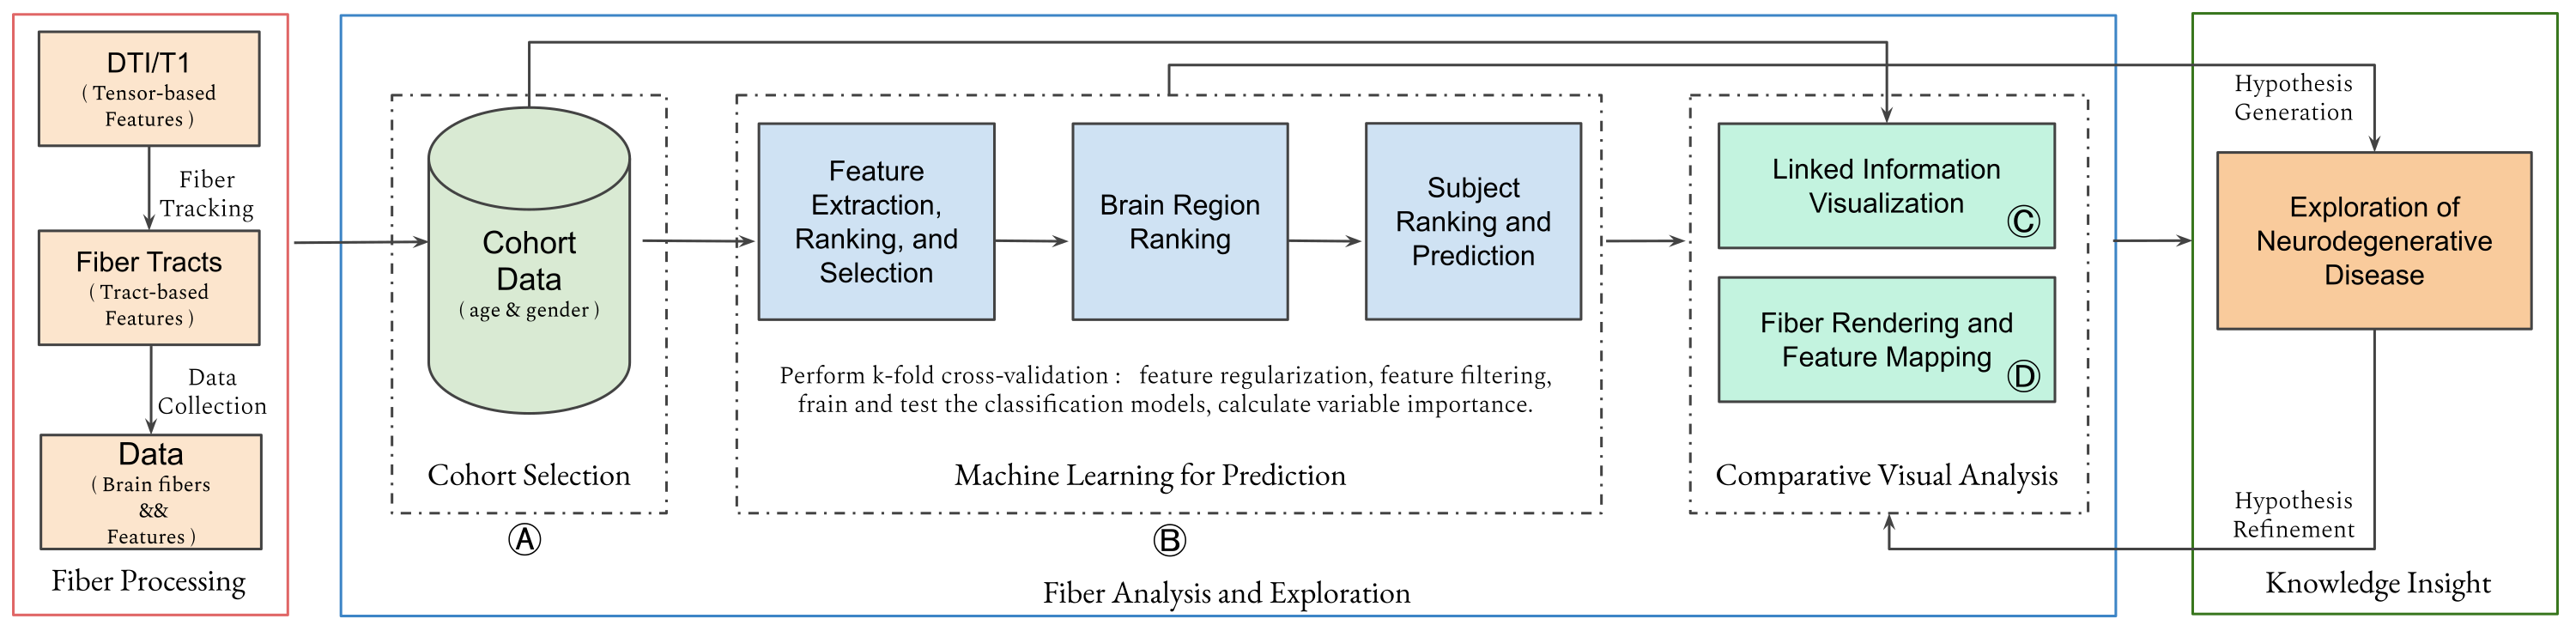
\includegraphics[width=1.0\textwidth]{images/Vis2020_Workflow.png}
%     \caption{A Schematic Diagram of the visual analytics process.}
%     \label{fig:workflow}
% \end{figure*}


%SystemVersion2.png
\begin{figure*}[ht]
    \centering
    \includegraphics[width=0.99\textwidth]{images/SystemVersion3.png}
    \caption{The UI of our visual analytics system. \clc{A} The cohort selection module supports balanced and stratified subject group selection and demographic analysis. \clc{B} The ML module can be customized before executed. The results (below) summarize the model performance and overall uncertainty. This includes an ROC curve, confusion matrix, the group sizes, and 4 difference performance measures: accuracy, precision, recall, and $F_1$. \clc{C} The interface for exploration includes 3 sub-modules: the region module, feature module, and subject module. They can each be toggled between plot views and table views as described in further sections. The values displayed include averages and standard deviations of the estimated silences and predictions. The subject view also encodes the class labels and binary predictions. \clc{D} The information visualization module includes a range of views for comparative analysis. \clc{E} The 3D fiber rendering views show selected subjects for physiological analysis.  The selected feature is mapped to the fibers through color; in this case a divergent color map is used and the mapped values represent the difference from the mean of the control group. Above each fiber view shows subjects' information and a timeline showing their mean values of the selected feature over time. The intervals on the timeline can be clicked to change the fiber view to display those different scans. Above the fiber views are adjustable rendering and viewing parameters, such as path tube thickness, camera linking, logarithmic scaling, and constrastive or direct value mapping.
    }
    \label{fig:system}
\end{figure*}

The aforementioned problems in neurodegenerative disease research have inspired the design goals for our system. \textcolor{blue}{Also, we reviewed challenges and future aims in neuroscience from several survey papers: 1) Many features identified using tractography have not been thoroughly verified in comparisons with the underlying anatomy in clinic research~\cite{thomason2011diffusion}. 2) A better understanding of the physiological changes in different brain regions and the detection of brain regions more focally using white matter fiber tracts~\cite{johnson2013neuromodulation, hampton2019substance}. 3) Identification of the differences between patients and controls, as well as the relations of individual patient to groups of patients and the differences that have great impact on disease progress~\cite{thomason2011diffusion, hampton2019substance}. 4) There's a necessity to provide  engineering guidelines to systematically explore white matter integrity in neurodegenerative disease~\cite{gold2012white}. To tackle these challenges, we made the design goals as follows:}


%The aim of this phase is to identify design goals of our system. We worked closely with five experts (two academic scholars at universities and three clinicians at hospital) with unique perspectives and backgrounds in neuroscience, including statistical analysis of neurodegenerative disease,  brain tractography from MRI images, diagnosis and treatment of PD. We have several round discussions from creating a common understanding between visualization scientists and the neuroscientists to iteratively designing the system based on the experts' suggestions. The distilled design goals for the brain fiber data analysis system are as follows: 

%The aforementioned problems in neurodegenerative disease research have inspired us to design goals for our system. With the experience of the researcher that has been working on brain fiber analysis in neurodegenerative disease for multiple years, we identified the design goals. While consulting neuroscientists in different research fields (e.g.,  PD and AD), they feel the design goals were reasonable and well worth the effort.
    
\begin{asparadesc}

    \item[DG1] \textbf{Guided analysis based on 3 modalities.}
   To facilitate an effective workflow, our system should help the user prioritize more salient (\textbf{a}) regions, (\textbf{b}) features, and (\textbf{c}) subjects to pragmatically choose subjects for detailed analysis. \textbf{d}. The regions and features should be standard and interpretable so that experts can more easily grasp the physiological basis, assimilate existing literature, and make hypothesis. \textbf{e}. Due to a large feature space relative to the number of scans, we must strive to avoid overfitting, reduce ranking instability, and highlight the uncertainties.
    
    % A large amount of features (e.g., hundreds of features) can be extracted from the whole brain for analyzing neurodegenerative disease. 
    % Therefore, a system should be able to suggest which features and brain regions have significant differences in the diseased brain when compared with the healthy brain. 

	\item[DG2] \textbf{Quality visualization of brain fibers.}
	For anatomical understanding, visual analysis of the fiber tracts and salient variables in the physical space is required. The rendering should be effective at showing structure, while also efficient enough to interactively render multiple large fiber sets simultaneously.
	
	\item[DG3] \textbf{Modalities for comparison.} Besides the explorative modalities that zero in on objects of interest, there are also multiple modalities for comparison of those interesting objects. These comparisons can help experts to relate the diverse and uncertain data in support of hypothesis development. 
%through the cohort study between diseased and healthy brains, 
	Targets for comparison include: group trends, group trends vs. individuals, multiple individual subjects, individual subjects over time, and correlations between variables. Furthermore, since we explore these facets based on estimated salience, we should also highlight their relationships to the driving predictive models. 

    % \item[DG4] \textbf{ Easy-to-use interactions with complex multi-faceted data.}
    \item[DG4] \textbf{Easy non-linear exploration.}
    Due to the large number of features, fiber tracts, and subjects, 
    diverse aspects could be explored. 
    The analytical process may proceed and change according to different patterns that emerge or knowledge that is discovered during the analysis. 
    Therefore, our system should provide an intuitive and fully interactive UI to serve the neuroscientists' changing analytics needs.

\end{asparadesc}

Using our teams' expertise (which includes machine learning, visual analytics, and fiber tract visualization), we made a prototype system.
% With the expertise of a researcher that has some prior experience studying fiber tracts in an interdisciplinary lab, we made a system prototype. 
Then, we consulted five experts in different research fields, including statistical analysis of neurodegenerative disease, brain tractography of MRI images, and diagnosis and treatment of PD. While consulting the neuroscientists, they confirmed our design goals and gave us feedback based on their unique perspectives and backgrounds. We then improved the system according to their feedback. 


% The following DGs (DG1--DG4) are identified to solve the problems described in Sec.~\ref{sec:problems}.
% DG1 and 2 correspond to Problems 1 and 2 in \autoref{sec:problems}, respectively. 
% DG3 and 4 are to solve Problem 3.\\

% \begin{compactdesc}
%     \item[DG1] \textbf{Identification of the most impactful features and brain regions to the disease.}
%     A large amount of features (e.g., hundreds of features) can be extracted from the whole brain for analyzing neurodegenerative disease. 
%     %They may affect the disease to varying degrees. 
%     Therefore, a system should be able to suggest which features and brain regions have significant differences in the diseased brain when compared with the healthy brain. 
	
% 	\item[DG2] \textbf{Quality visualization of the brain fiber tracts.} 
% 	To help anatomical understanding of the disease, visual comparison of the fiber tracts between the diseased and healthy brains is required as well as comparison with statistic features. 
% 	Thus, a system should provide a high quality 3D visualization of the fiber tracts in a user-selected brain region.
% 	%A spatial region based analysis which combines 3D rendering of brain regions with statistic measurements of interest that selected by users mapped to the physical structures would help in an anatomical understanding of the disease. 
	
% 	\item[DG3] \textbf{Overview of relationships between subjects and features.} 
% 	To build a hypothesis through the cohort study between the diseased and healthy brains, a system should provide a visualization of the relationships between subjects and the extracted features. 
% 	Because there will be potentially many different subjects and features, the visualization should provide an overview of the relationships based on the user's need.
% 	%The measurements, to a large extent, can be used to analyze the disease, however, it lacks of gaining the relationship between variables as well as it lacks the overall trends in all the subjects. 
% 	%An overview of all the subjects and distribution of the variables that have a profound impact on the disease can help in the understanding of both the disease and the healthy groups. 
	
% 	%\item[DG4] \textbf{Comparison across subjects and different time steps of a subject.} Although the physical structures and variables can be well observed and understood, researchers cannot make any judgments about the disease without comparison. The comparison between different subjects and different time steps of a specific subject allow researchers discovering the laws of the disease and judging the disease more reasonably. 

%     \item[DG4] \textbf{ Easy-to-use interactions with the complicated data.}
%     Due to the large number of features, fiber tracts, and subjects, there is a wide variety of aspects that could be explored. 
%     The analytical process may proceed and change according to different patterns that emerge or knowledge that is discovered during the analysis. 
%     Therefore, a system should provide an intuitive and fully interactive UI to serve the neuroscientists’ ever-changing analytics needs.
    
% 	Because neurodegenerative disease usually changes over time and it also manifests in individual differences. An observation of per subject trends of disease progression is needed. Furthermore, simply by observing the progressive changes of specific subject in disease will lead to inaccurate judgment. Comparison of measurements across subjects or groups is required. 
%	\item avoid over-fitting and generalization error 
% it seems like the simplest way to increase stability of feature selection is to use something like Random Forrest or other ensemble based methods. This is already implemented in Sci-Kit learn as well. The other recommendation is to group correlated features, or remove redundant ones. It would be nice to handle that, but dealing with feature groups requires more work and features in our system for visualizing and analyzing these groups. For now I will just switch to some ensamble methods. In the writing, I will list 3 requirements (1) account for the selection bias problem inherent in high dimensional data such as ours. (2) Account for selection/ranking stability (for features, subject predictions, brain regions). (3) Avoid pitfalls of circular analysis. We could possibly add these requirements to the existing requirements section, as well.




% \begin{figure*}[!ht]
% \centering
% 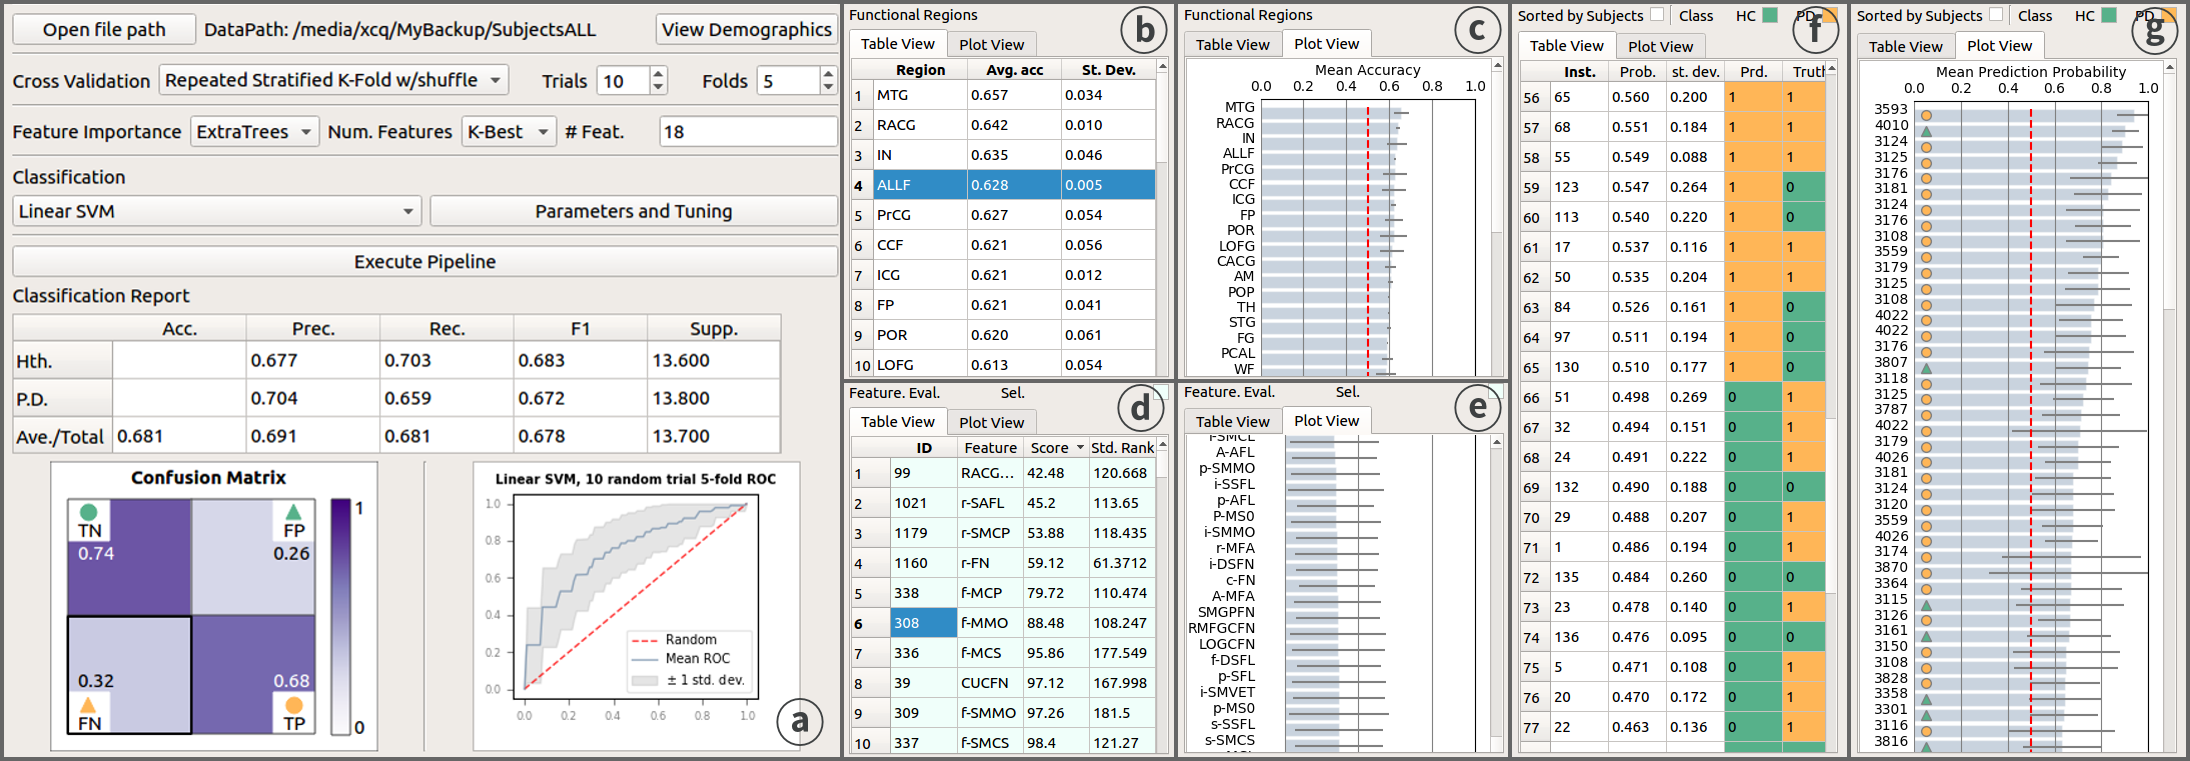
\includegraphics[width=0.9\textwidth]{images/Module_MachineLearning.png}
% \caption{The prediction performance chart in our system. (a) shows the parameter setting for feature filtering, feature reduction, feature ranking and classification. The confusion matrix is shown( left on the bottom), along with the ROC curve(right on the bottom). Brain region ranking and selection are shown in (b), which the regions are arranged in order of accuracy. (c) shows the features that have been ordered by ranking, the top-k highest ranked features have been colored light-blue. (4) shows the subjects that have been ranked according to the predicted probability that they have the disease.}
% \label{fig:MachineLearning}
% \end{figure*}



% \section{ML for Prediction}

% \TF{Many of the parts are not clear if we do not explain the dataset, views, and interactions. So, I suggest that (1) we should explain the dataset in the first subsection (with some description about our system is still desinged for any datasets.) (2) explain each subsection with the corresponding view and interactions. Also, still I don't get it why we want to predict something. (what do we predict? and why do we want to predict it?). Somewhat I understand about the reason, but still it seems not straight forward (i.e., we know the answer, then try to predict PD or not using the selected variables, then find which one is more likely distinguish PD or not. Then, we can more focus on analyze that variable, region, etc.).}.

% \subsection{ Dataset }

% Current dataset contains 140 data, including 69 health group data and 71 disease group data. The demographics of the 2 groups have been compared in Fig.~\ref{fig:demographic}. Due to neurodegenerative diseases are usually age-related, both healthy and disease groups must have similar age distributions. Gender is also within the scope of consideration. In both groups, the amount of male subjects is more than that of the female. "The incidence of Parkinson's disease is low before the age of 50 years, but it increases rapidly with age, peaking in most studies at around 80 years, probably because of underdiagnosis with increasing age" -- this sentence is copying from another article

% Afterwards, we dig out features for each brain data. The features that we obtained fall into 2 categories: tract-based features and tensor-based features. Tract-based features include features based on the number of fibers and fiber length, which are commonly used indicators in brain disease investigation\cite{sundaram2008diffusion}. The tensor based features are the tensor measures calculating from the a diffusion tensor model at each voxel in DTI images, such as Fractional Anisotropy (FA) value, Mean Diffusivity (MD) value and Radial Diffusivity (RD) value, which are widely used in the detection of brain disease\cite{ji2015white}. The whole brain is segmented into 42 regions based on a brain atlas which assigns neuroanatomical labels to each brain functional regions. Fiber tracts and the corresponding tensor measurements are obtained after fiber tracking. Since it has been reported that disease starts from one region and then spreads to other areas, in order to better detect how the disease progresses, we further divided the fiber tracts into 2 categories: inner connect and inter connect fibers. inner connect fibers are fibers in which the start and end points are both located in the same region. Also, since cortical asymmetry and hemispheric predominance have been discovered in neurodegenerative disease \cite{scherfler2012left}, the features `Delta-LR'(the delta value of left brain and right brain) were included to represent the differences between the left and right hemispheres. We calculated those features of different brain functional regions separately. Cumulatively these features amount to about $1,800(42\times2\times14 + 42\times13 + 7\times13 + 4 )$. 42 brain regions, 2 types of fiber tracts (inner connect fibers and inter connect fibers), 14 tensor based features, 13 fiber based features, 7 lobes, and 4 demographics.

% Due to such amount of brain data and each brain contains quite a lot of features, there is a necessity to introduce ML to help identify which features are meaningful for distinguishing the brain disease.

\section{Methods} 
\label{sec:methods}

% The driving mechanism of our system is a predictive modelling pipeline that helps the user identify salient brain regions, fiber tract features, and subjects to prioritize for analysis. This pipeline is integrated as an interface to support intelligently guided VA through those 3 exploration modalities (DG1). The interface is coupled with multiple linked information visualizations and 3D rendering views to support a wide range of comparative modalities (DG3). The comparative modalities and supporting visualizations are chosen to offer a holistic view that provides the context an expert may need to reason about the complex and uncertain information they are presented with. 

\noindent We begin with an overview of our system before going through the detailed design and implementation.

% In this section we describe our methods in detail, and how these different components are linked together to provide a cohesive VA system.

% \subsection{Overview of Our Approach}
\subsection{System Overview}
\label{sec:systemoverview}

% First we give a high level introduction to our system and explain how each of the system components relates to the design goals. 

%\autoref{fig:workflow} 
\noindent Fig.~\ref{fig:system} shows our VA workflow and UI. A preprocessing step includes fiber tracking and feature extraction. In the system, the user begins by selecting cohorts through a module that balances the subjects in each group while stratifying with age and gender (Fig.~\ref{fig:system}\clc{A}). 
%The user then validates the cohort selection by through by opening a view for visual comparison.

Next, the user initiates the ML pipeline depicted in Fig.~\ref{fig:system}\clc{B}. This generates saliency measures for each of the 3 exploration modalities through the following process, repeated for each brain region separately: Through a number $c$ of stratified and randomized $k-$fold cross validation (CV) loops 
%(a method to split the data into different combinations of training and test sets),
%( Sec.\ref{sec:pitfalls})
, estimate each feature's salience based on the training data,  train a classification model based on the top $m$ features, use the trained model to predict the labels of the test data, and record the feature scores, modeling performance (for region saliency), and the probabilistic predictions for each individual subject. 

Afterwards we have $c\times k$ sets saliency scores for each modality; we then compute the averages and standard deviations. The overall modelling performance is summarized in Fig.~\ref{fig:system}\clc{B}, and the saliency scores update the region, feature, and subject exploration modules in Fig.~\ref{fig:system}\clc{C}. As the user explores using these modules, interactive visualization views are generated based on the user's selections, including linked information visualizations and fiber views (Fig.~\ref{fig:system}\clc{C},\clc{D}). 

% The workload is distributed over multiple parallel processes, with each process working on a different region. 

% By increasing $c$, more randomized CV loops are executed (testing more random combinations of test-train data), which will result in better estimation of the uncertainty at the expense of longer wait times to get back the results (see Sec.~\ref{sec:methods}). The process may take several minutes or more depending on number of features, subjects, and CV iterations. 

%This process and workflow provides a solution to our first design goal DG1.


% To support DG2, our system includes a 3D visual comparison view, that can show multiple brains at once with linked camera's. The region that is rendered is automatically selected based on the user's selection from the region importance view. The color mapping of the fibers is based on the feature/variable from the feature importance view. And the compared subjects are based on selections from the subject prediction view. To support efficient, quality rendering, a GPU shader pipeline is used, which includes a geometry shader that converts line data into path tubes, which have an interactively adjustable radius; and screen space ambient occlusion is used to efficiently render lighting with shadows that give better depth perception. These features provide a solution to DG2, and also help support DG3 and DG4. These views are shown in Fig.~\ref{fig:system} \glf{E}.

% Next, as shown in Fig.~\ref{fig:system} \glf{D}, linked information visualizations are used in our system to help support DG3 and DG4. The primary visualizations that are featured in this part of the system include a parallel coordinates view, a specialised scatter plot view that shows the average predicted probabilities of each subject vs their trends in a selected feature, and a group-wise histogram comparison view. The parallel coordinates view helps to support group level comparison of the trends of the top features in addition to comparison of selected individuals features with the group trends. The scatter plot view helps to analyse the relationship between the model, the features, the individual subjects, and the group trends. The histogram view is a simple but useful view, that clearly shows how much overlap/similarity there is between groups in the selected feature. Other visualizations in this module include a correlation matrix and dimensionality reduction. Interactions on these views, the encodings that are used to represent and identify individual subjects throughout these visualizations, and the rest of the system are described in Sec.~\ref{sec:methods}.



% As shown in \autoref{fig:workflow}, brain fiber tracts and their features are collected by the preprocessing step indicated with the red rectangle.
% This step performs fiber tracking on the MRI images including DTI and T1-weighted images, which are commonly used medical image data for brain disease analysis. 

% In order to identify the most effective features and anatomical structures to the disease (DG1), the ML pipeline has been applied for ranking the features, brain regions, and subjects.
% Bases on the predictions, it can produce new hypothesis for researchers in disease exploration. 
% Based on the rankings, the neuroscientist can select specific features and brain regions and analyze relationships across the features, fiber shapes, and disease (DG2) with the information visualizations and 3D fibers. 
% Several linked information visualizations have been provided for showing both of the overall distribution of the features and subjects, as well as showing the relationships between the variables (DG3). 
% In addition to the visualization in population, we also support the comparison across individual subjects. 
% With fiber tracts are rendered side by side in the 3D rendering view and the timeline views of a selected subject, users can intuitively visualize the difference between 2 subjects and observe the progressive changes of a subject.
% Finally, it allows for the verification and exploration of the hypothesis, through the comparative visual analysis of brain fibers and their features in the spatial domain (DG4). 

% Fig.~\ref{fig:system} is the interface of our system that depict how the analytic workflow works.  (A), (B), (C), and (D) show each steps of fiber analysis and exploration, separately. Firstly, all the data have to be loaded and ML methods have to applied to those data. As shown in module (A), researchers are allowed to pick out subjects of certain age range and select classification model for prediction. Secondly, users are allowed to explore the feature that they are interested in according to the prediction results. Module (B) shows the features, brain regions, and subjects that are displayed in a list. Users can manually select the features based on their ranking and prediction for exploration. Thirdly, as shown in module (C), linked information visualizations have been used in our system to show the distributions of the features and subjects. Users can gain an overview of subjects and variables in population. Fourthly, see in module (D), with the 3D rendering of the fiber tracts and the timeline views of the selected subject, users can intuitively visualize the difference between 2 subjects. %users can intuitively visualize the 3D rendering of the fiber tracts with the features mapped to the fiber tracts. Moreover, the timeline views allow users directly visualize the progressive changes of a subject.

\begin{figure}[t]
\centering
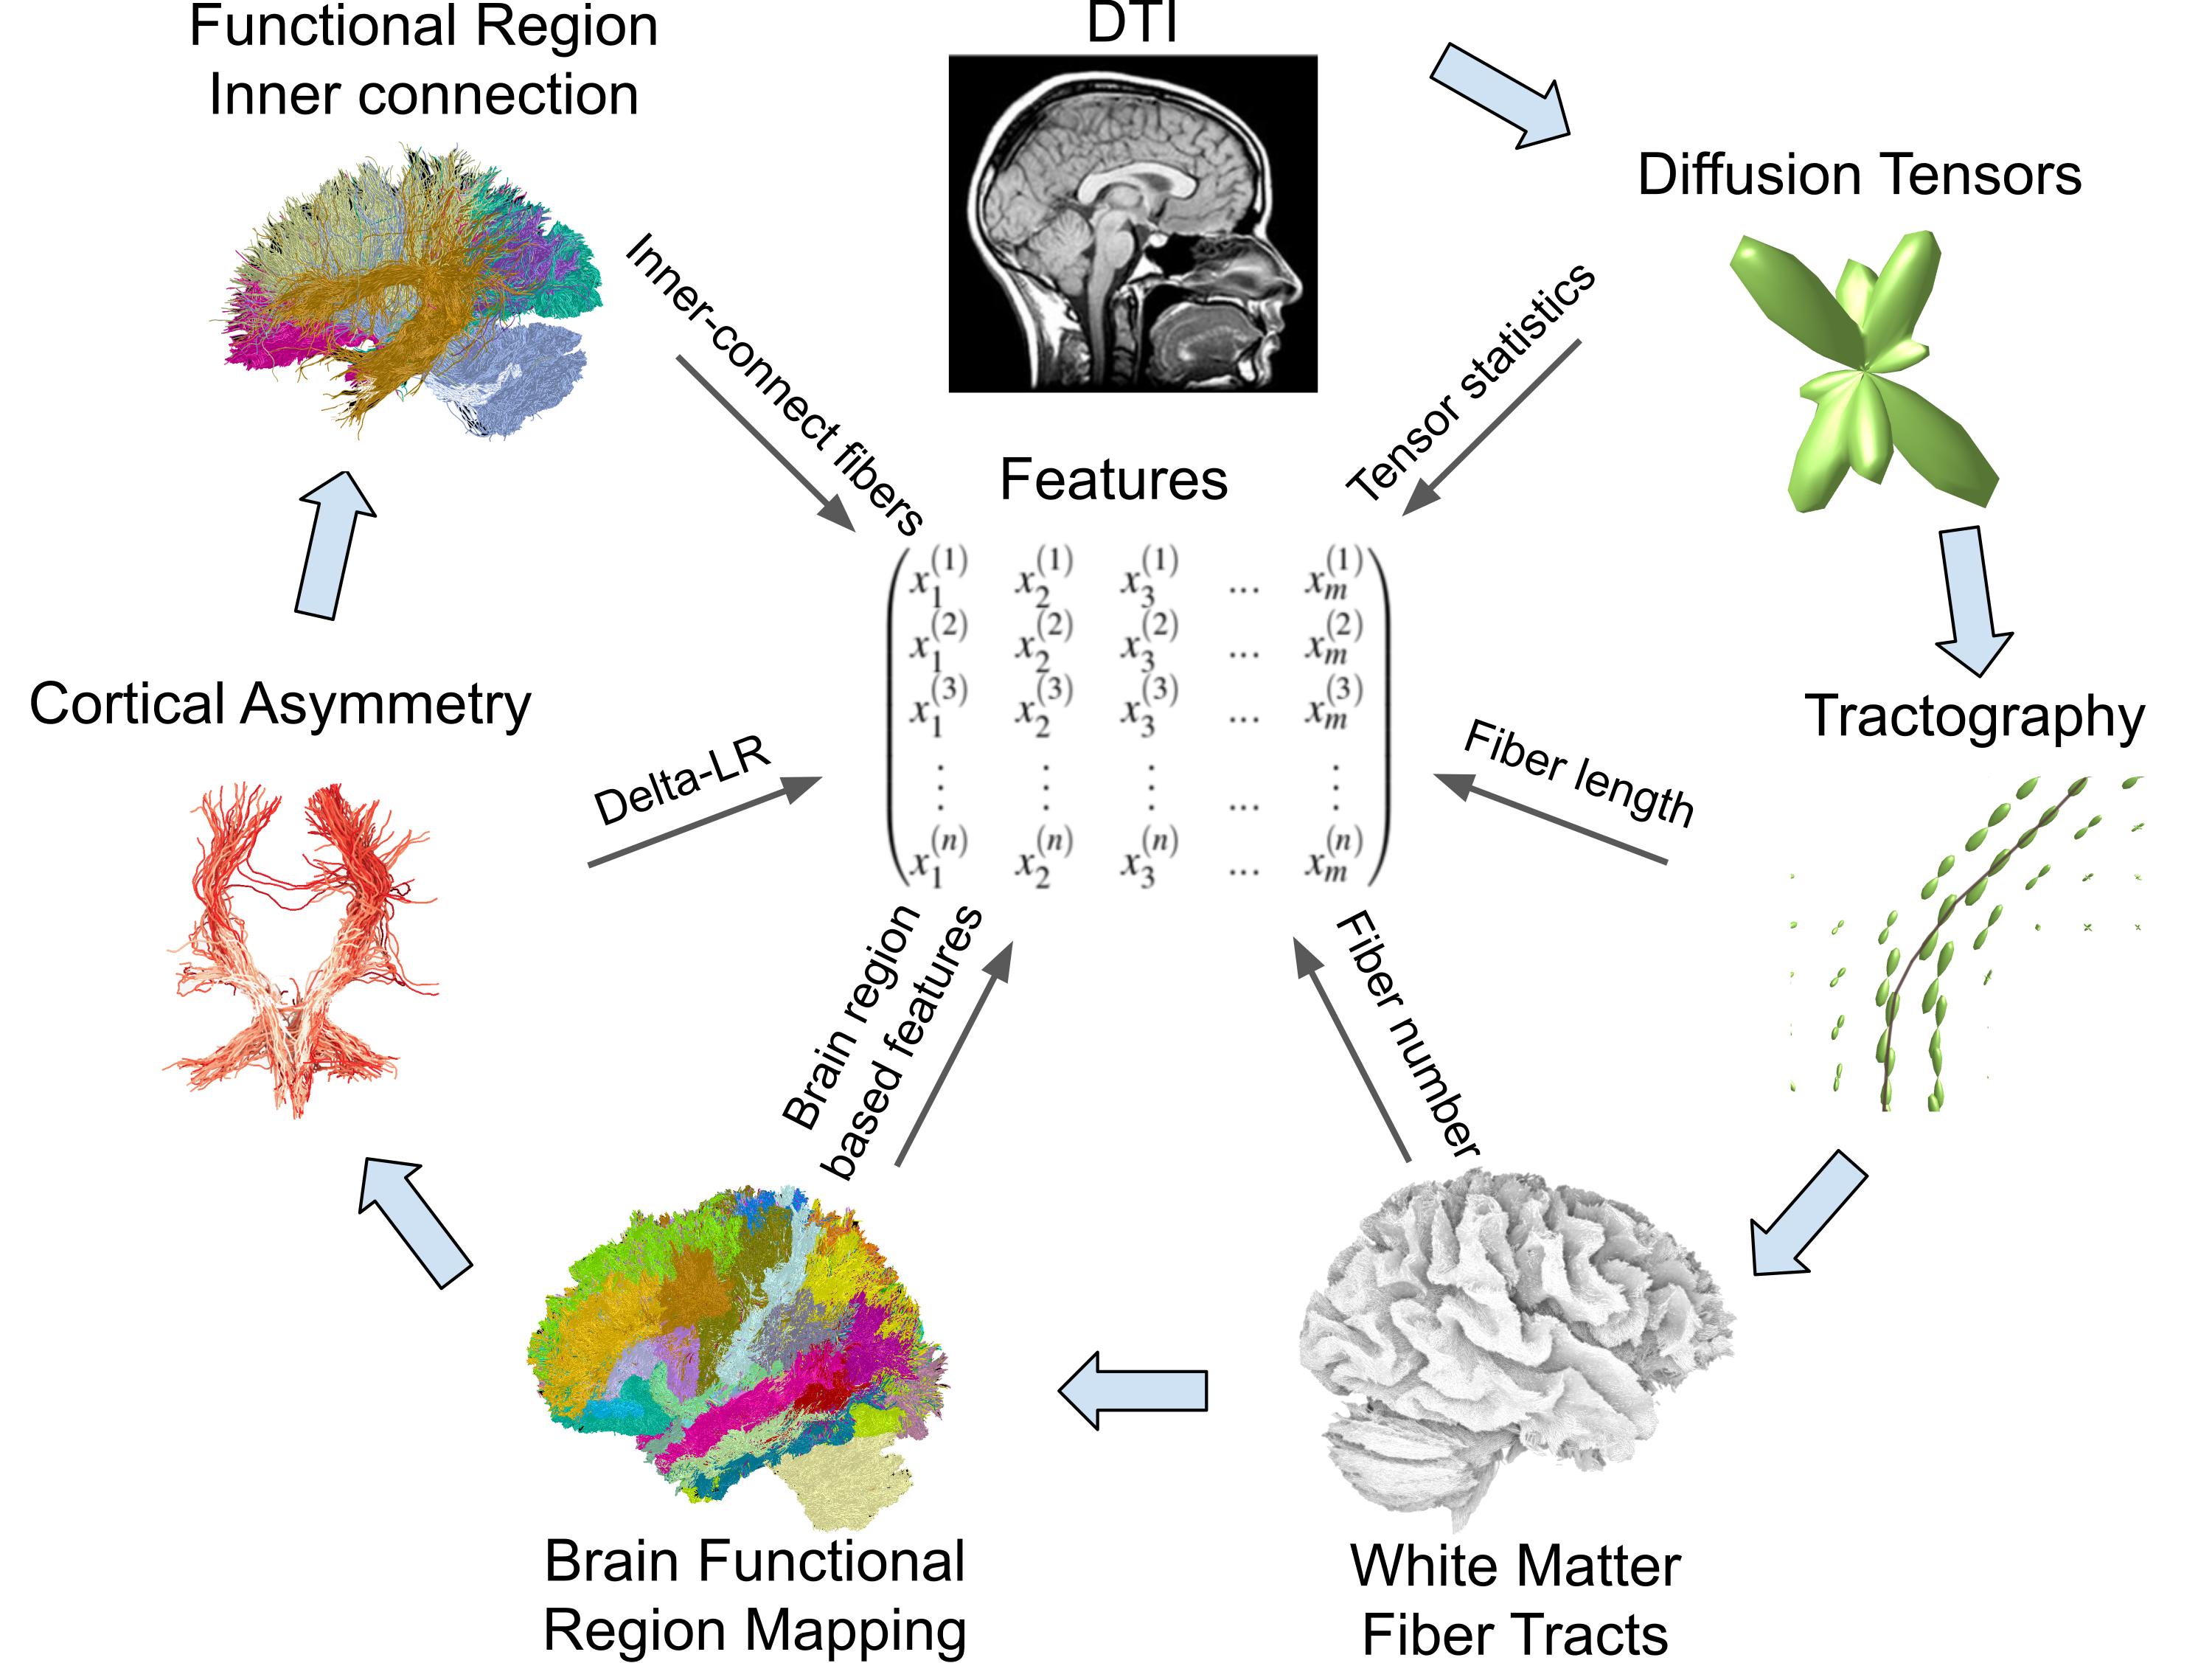
\includegraphics[width=0.95\textwidth]{images/Brainfeatures.png}
\caption{The feature extraction process described in Sec.~\ref{sec:extraction}.
% Feature extraction. White matter fiber tracts are reconstructed from tensors contained in DTI images (which measure water diffusivity). Functional region mapping provides anotomica by the regions. discover the cortical asymmetry of the brain, and show the inner connected fibers of each brain region. The features ranging from tensor fields to fiber tract fields are extracted from each steps of the pipeline.
}
\label{fig:Extraction}
\end{figure}

% \begin{figure}[h]
% \centering
% 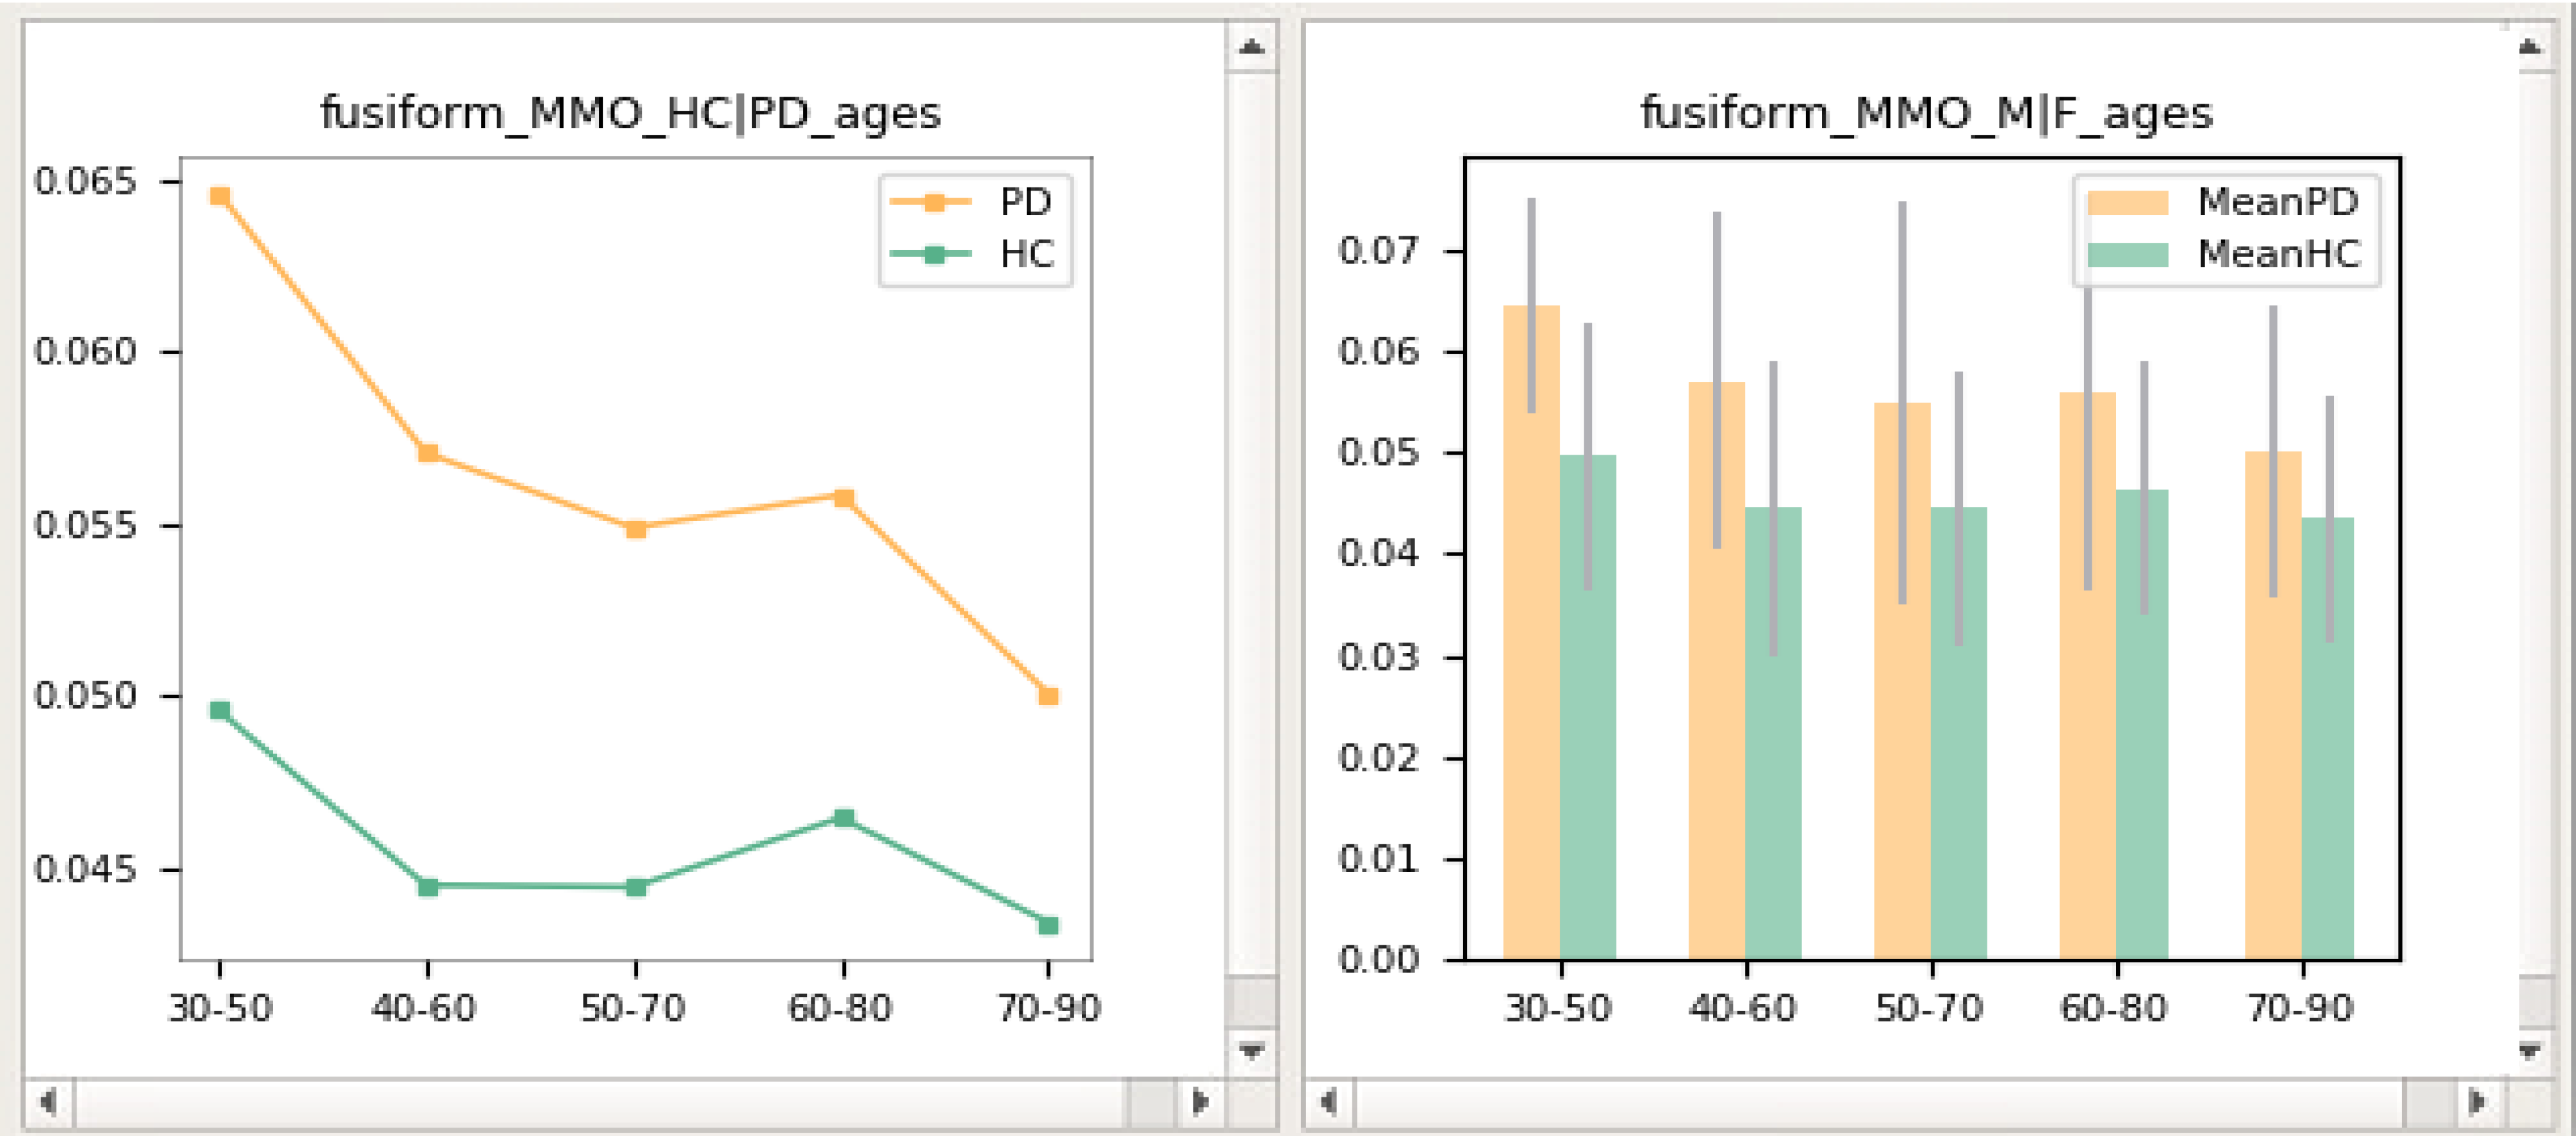
\includegraphics[width=0.85\textwidth]{images/line_Bar.png}
% \caption{Group level comparison of the trends of the selected feature and brain region. The left plot shows a line chart of the MMO feature trends in fusiform region between the 2 groups with age growth, while the bar chart one also aware of uncertainties.}
% \label{fig:line_bar}
% \end{figure}

\subsection{Feature Extraction and Fiber Bundling}
\label{sec:extraction}

\noindent We extract features for ML in a preprocessing stage using Mrtrix3~\cite{TOURNIER2019116137}. They fall into 2 categories: tract-based and tensor-based. The former measure regional fiber structure (e.g. density and length), while the latter measure water diffusivity based on a tensor model (e.g. fractional anisotropy (FA) 
%mean diffusivity (MD), 
and radial diffusivity (RD)). Evidence suggests that both categories are affected by neurodenerative disease~\cite{sundaram2008diffusion,ji2015white}.
% Due to the tensor measures are contained in the DTI images, tensor-based features will not be affected by the number of fibers. 

Fibers are bundled based on neuroanatomical labels assigned using a 42 region brain atlas. Also, since PD has been reported to start from one region and then spread to others, 
%features representing connections are worth investigating; thus,
we further divide the bundles into 2 categories: intra-connect and inter-connect (connecting to same or separate regions). Also, since cortical asymmetry and hemispheric predominance have been discovered in neurodegenerative disease \cite{scherfler2012left}, the features 'Delta-LR' are extracted to represent asymmetry between the left and right hemispheres. Tensor-based features are averaged over the different bundles of fibers (Fig.~\ref{fig:Extraction}).

Our choice of features is motivated by literature review and to favor interpretability, follow standard conventions, and support fiber tract based analysis (\textbf{DG1d}). It would also be possible to use dimensionality reduction methods such as PCA and or LDA to derive a reduced feature space. However, the resulting linear combinations may not be readily interpretable. Another approach is deep-feature learning. This may be a good direction for future work, however this would also cause difficulty for interpretation and assimilation. Still, our VA system is decoupled from feature extraction so alternative feature sets can be used easily. 
%, however it is important that the features can be rendered in physical space. 

% \subsection{Confounding Factors}

% The first stage of our pipeline involves an analysis and balancing of external factors within the population (e.g. age and gender). Besides balancing these factors between the control and disease classes, understanding the distribution of these factors is important for assessing the uncertainty and limitations of the end results. Therefore, this step is an important preliminary stage, which may also sometimes prompt the user to go back to the data collection phase before proceeding with the analysis.

% Within our UI the demographics are visualized as a pop-up view that shows histograms of the demographics. The view is opened automatically when the analysist first selects the dataset, and can also be opened again manually at any point.

\subsection{Cross Validation}
\label{sec:CrossValidation}

% {\color{red} proofread up to here: need a simpler explanation of CV, compare with bootstrapping, discuss bias-variance trade-off.}

\noindent Over-fitting a model to a data sample can reduce its ability to generalize to an unseen population. The severity increases with data complexity and limited size. For example, more features creates greater risk that by-chance fluctuations could discriminate target labels~\cite{krawczuk2016feature}. An over-optimized model, learned to exploit those fluctuations, leads to what's called generalization error due to variance. Model simplicity (under-fitting) reduces that error term, but increases what's called generalization error due to bias.
%(e.g. if most $x$ are $y$, then treat all $x$ as $y$). 
The conflict between these two error terms is called the bias-variance trade-off. This issue is an important factor for designing our ML pipeline to support \textbf{DG1e}.

Estimating generalization error (validation), is done by re-sampling into separate test and train samples. Bootstrapping (repeated sampling/testing with replacement), is a good variance estimator, however it tends to poorly estimates bias. Another approach is CV, which samples without replacement. $k$-fold cross validation is a popular variant, which splits the data uniformly into $k$ subsets and rotates their role as the test set $(k-1)$ times. CV gives good estimation of bias, but tends to be sensitive to variance due to a dependency on the partition. Stratification (optimizing representativeness between subsets) helps reduce this sensitivity to a point. Another variant of CV, repeated randomized test-train split, offers an improvement in variance estimation. This has been found to work well compared with $k$-fold CV for neuroimage data~\cite{varoquaux2017assessing}. This makes sense since variance is major problem in neuroimage data due to high complexity and small sample sizes. 

\begin{figure}[t]
\centering
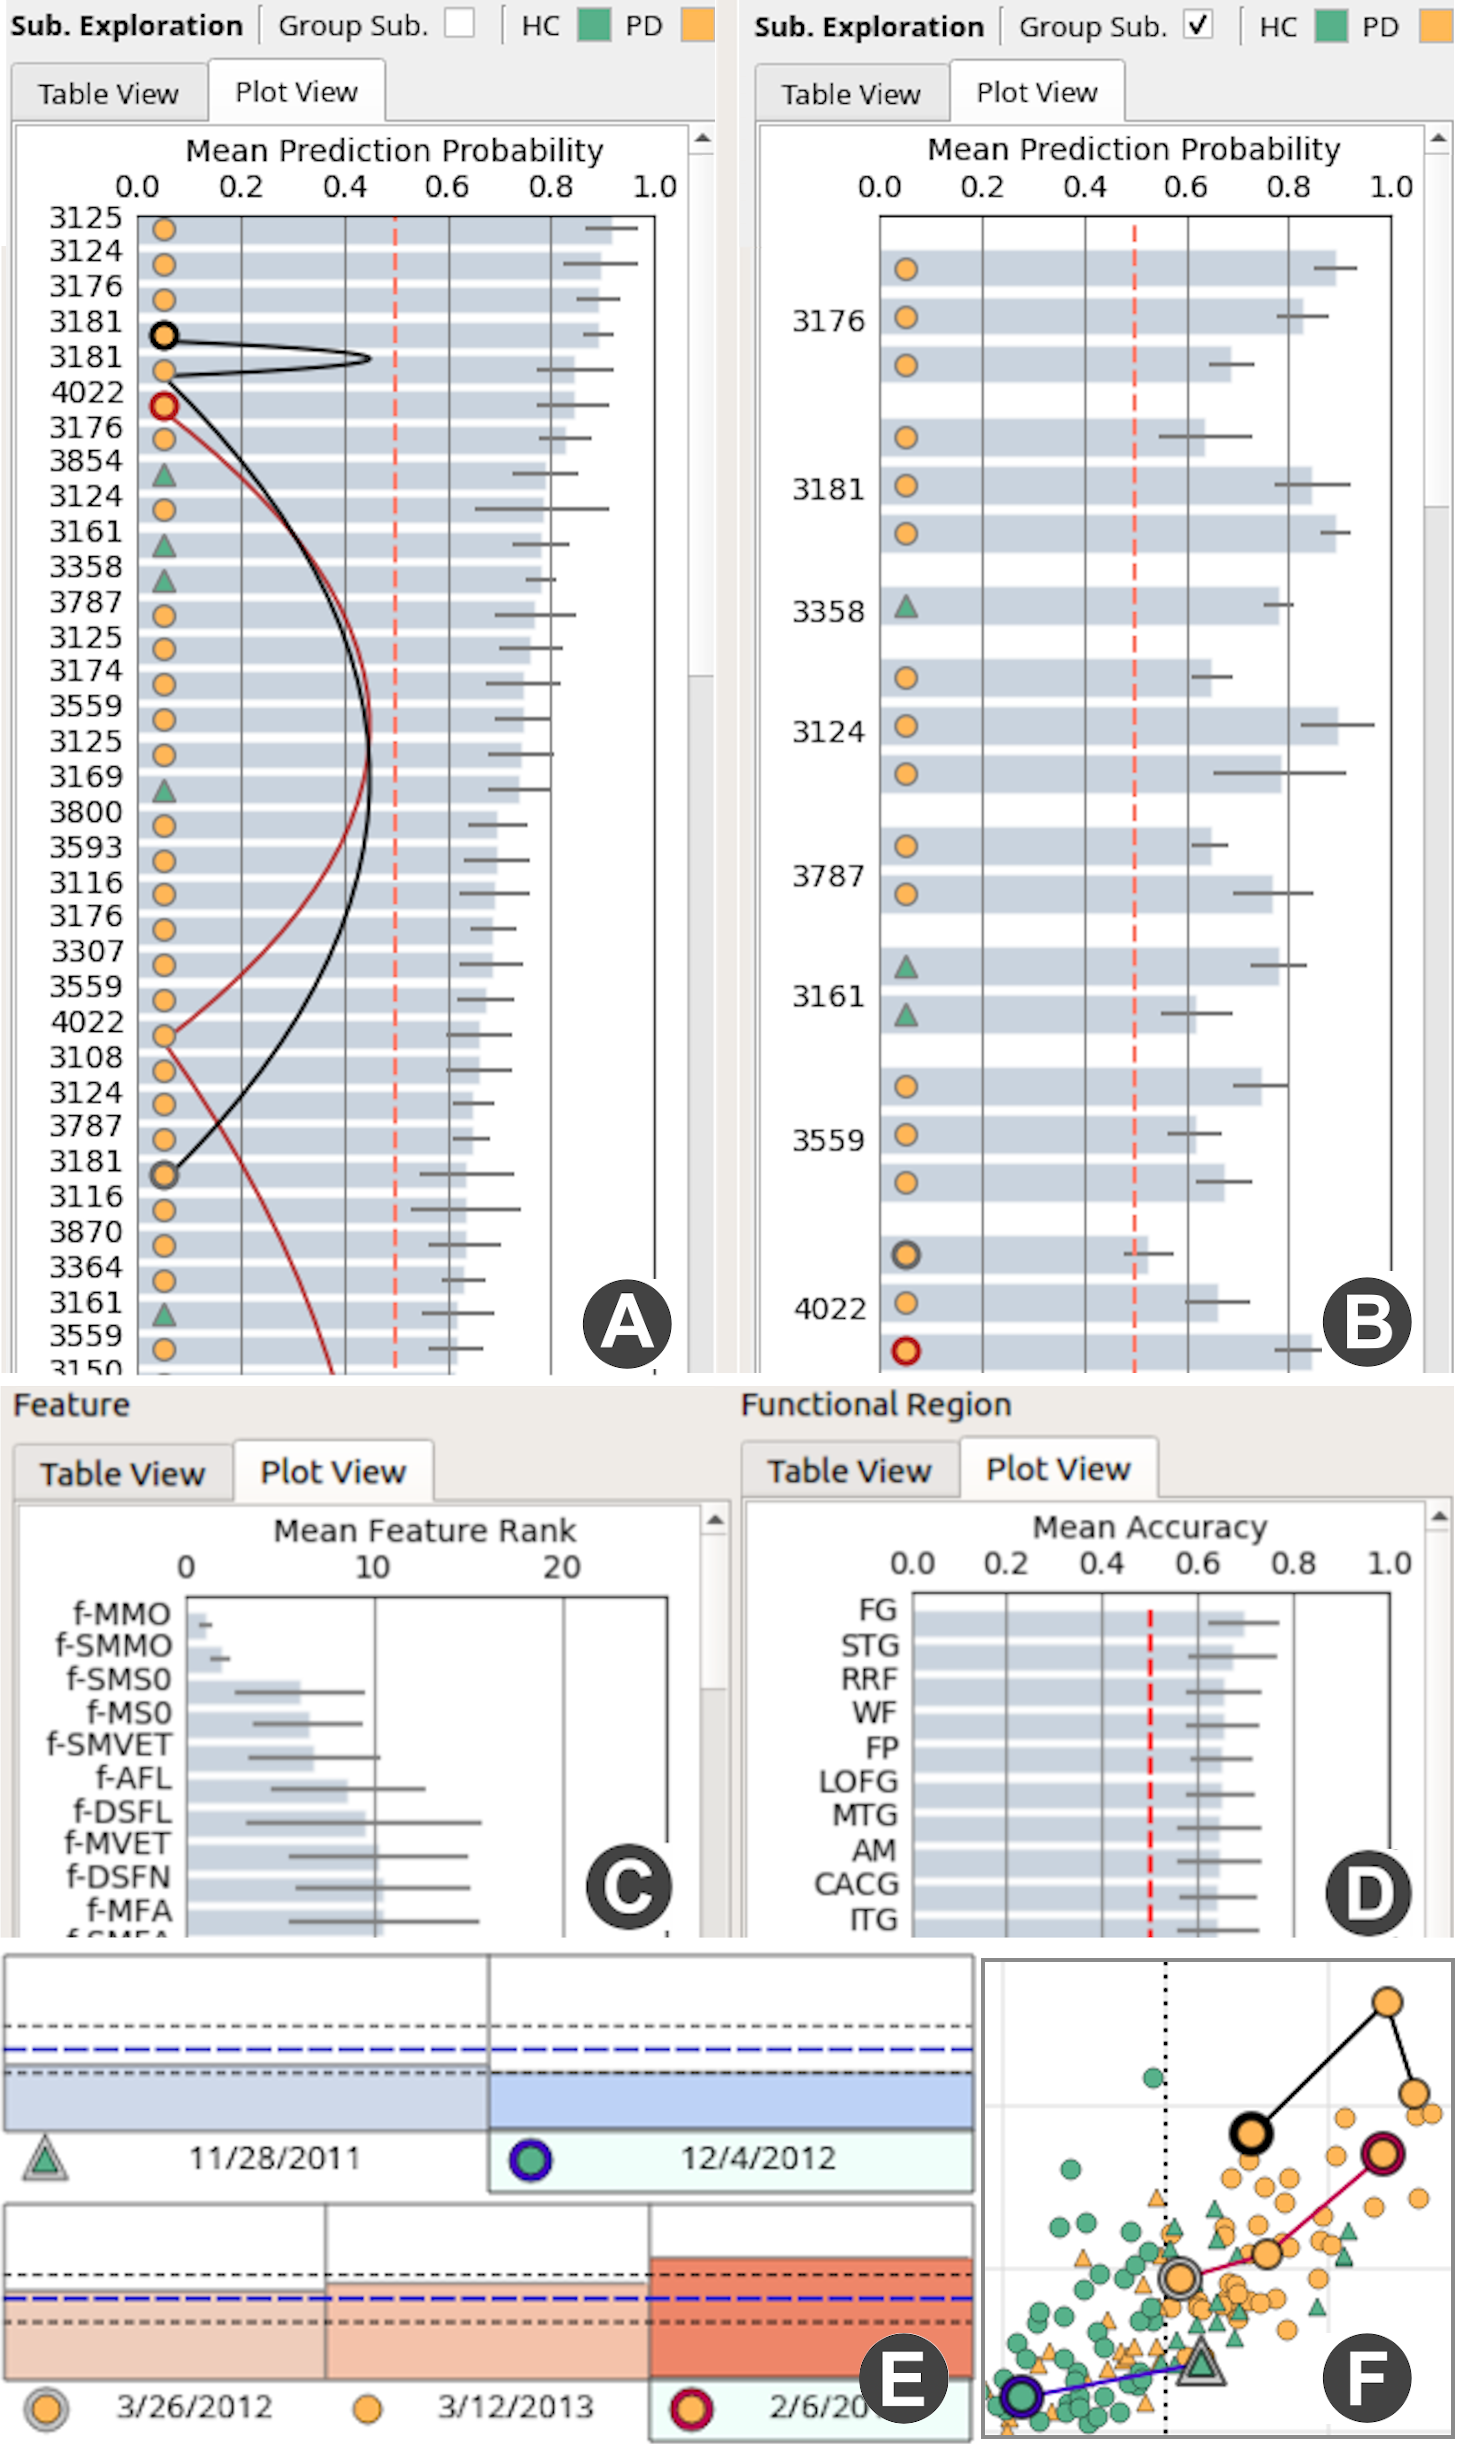
\includegraphics[width=0.95\textwidth]{images/plotView4.png}%
\caption{Plot views of exploration modules and across-view encodings. Glyphs: orange and green fill color encode healthy and disease respectively, circle and triangle encode correct and incorrect prediction, thick borders distinguish compared subjects, their currently selected visits, and which of those visits is the earliest. In this case, dark-blue, dark-red, and black indicate which subject is visualized in the left fiber view, right fiber view, and is mouse hovered in a plot view, respectively. The thick border is colored (blue, red, black) only for the subject's currently selected visit, while their first visit is grey (unless it's selected), and the other's have no thick border. As necessary, lines/curves then connect those glyphs associated with a single subject's multiple visits/scans (\glf{A},\glf{F}), and disambiguate the temporal order. \glf{A} Plot view of subject exploration module sorted by class prediction probability. \glf{B} Same view grouped first by same subject; i.e. their multiple visits are grouped, those groups are then sorted by average prediction, and within group by visit date in increasing order from top to bottom. \glf{C} Plot view for feature saliency. \glf{D} Plot view for region saliency. In plots \glf{A}, \glf{B}, \glf{C}, and \glf{D}, the blue-gray bars encode average score while the thin gray bars encode the standard deviation. \glf{E} The subject time-point selection modules (attached to the fiber views~Fig.\ref{fig:system}\clc{E}) display selected feature over time, and supports switching between those visits. The dotted blue line is the average of the control group, while the black dotted line shows standard deviation.}
\label{fig:subjectsUncertainty}
\end{figure}

One of our objectives is subject level exploration (\textbf{DG1c}) using probabilistic predictions, as described further in Sec.~\ref{sec:subjects}. However, both bootstrapping and repeated randomized CV cannot guarantee that each subject appears in a test set an equal number of times. Standard $k$-fold cross validation does guarantee this, but also may suffer from sensitivity to variance (which is a particular problem in our domain). For these reasons, we use an extension of $k$-fold CV, performed $c$ times with randomization. This allows equal testing of subjects ($c \times (k-1)$ each), and also supports good modelling of the uncertainty/variability. 

Note that choice of $k$ determines the relative sizes of test and train sets at each CV iteration; a smaller $k$ will result in lower representation of the variance in the test-sets, but increased representation of the variance in the training sets. A larger $k$ also results in more overlap in the training sets between each CV iteration. The larger training sets will tend to give a better estimation of the overall performance, and the overlap will tend to cause more consistent between iterations, but in turn may underestimate the variance (giving a false sense of stability). In smaller samples, it's also important that the test sets are representative, which implies a small enough $k$ should be chosen. Ultimately this is a complex trade-off, which is highly data dependent. Based on our goals, the literature, and experiment, we choose a default of $k=5$, which we found to strike a good balance. It can be adjusted within the system based on special consideration by expert users.

% While a smaller $k$ may underestimate the models performance (since less training data is used in each iteration), it may result in more stable estimations that are less affected by variance between test sets (so long as train sets are still representative enough). Erring on the side of stability is desirable for our case, since the data has high-complexity relative to sample size, and our goal is prioritized VA (which benefits more from stable relative saliency estimation than overall performance estimation). 


% One possibility is to separate feature saliency estimation from model training. However, we go against this choice since we aim to also support feature analysis in relation to the classification model in one mode of comparison (\textbf{DG3}). Although it would be possible to include additional saliency measures that have not informed the predictive model, we felt that this may be confusing or easy to misinterpret.

% A popular default for neuroimage data in the literature is $k=5$. For $c$, we use a default of $10$, which is enough to provide strong estimation of the variance, while incurring a reasonable run-time overhead. 
%Besides the outer CV loop, an inner (nested) CV loop~\cite{varma2006bias,varoquaux2017assessing} is used for hyper-parameter tuning and model based feature selection (which require test and train samples that are independent from the outer CV test sets).% Since the inner CV loop splits the training data in the outer CV loop into test and train sets, we must choose a $k$ value for the inner loop as well, and the bias variance trade-off in this inner loop is also affected. This implies a conflict between the benefit of choosing a smaller $k$ in the outer loop (which favors better stability) since if gives less data for the inner loop to work with (acting against stability in the inner loop). 

%Collectively, these choices do well to address \textbf{DG1e}. %Our approach also helps address stability in region and feature ranking~\cite{saeys2008robust} as discussed in the next 2 sections.

% \begin{figure}[!ht]
% \centering
% 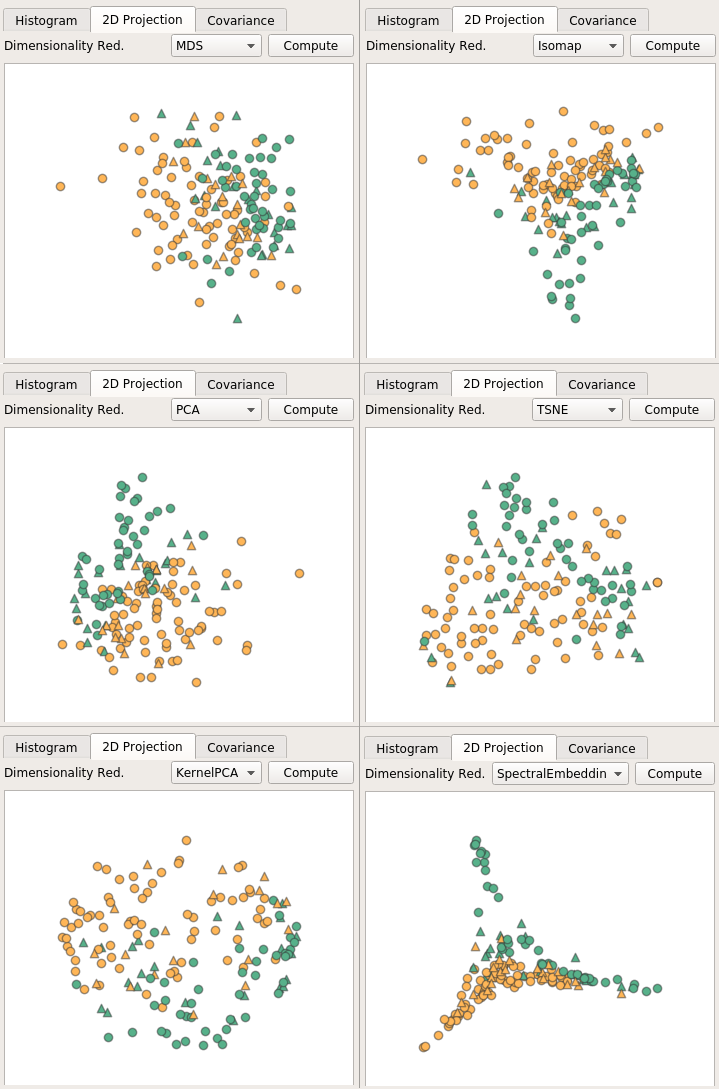
\includegraphics[width=0.9\textwidth]{dimensionalityReduction.png}
% \caption{Our system includes $6$ options for projecting the selected features into 2 dimensions for visualization. Each method appears to work well for separating the 2 groups. Orange shows the disease group, blue-green shows the control group. Triangles represent false prediction, while the circles represent true predictions}
% \label{fig:dimensionalityreduction}
% \end{figure}


% \begin{figure}[!h]
% \centering
% 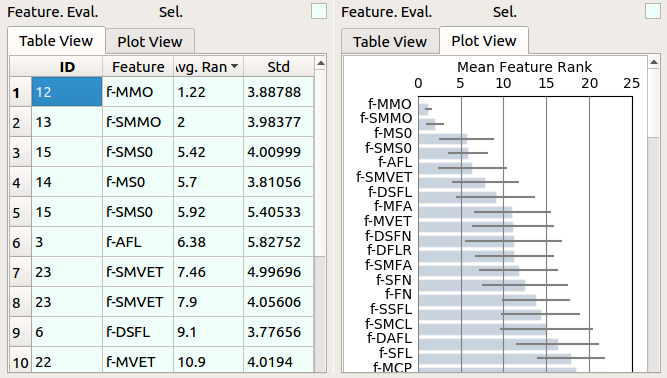
\includegraphics[width=0.9\textwidth]{images/featureRanks.png}
% \caption{ Table view and plot view of the predict features. Table view shows features that are sorted by average ranking followed by standard deviation, while in the plot view bar chart are sorted by the average prediction accuracy and error bars indicate the standard deviation of each feature.}
% \label{fig:featureRanks}
% \end{figure}


% \begin{figure}[h]
% \centering
% 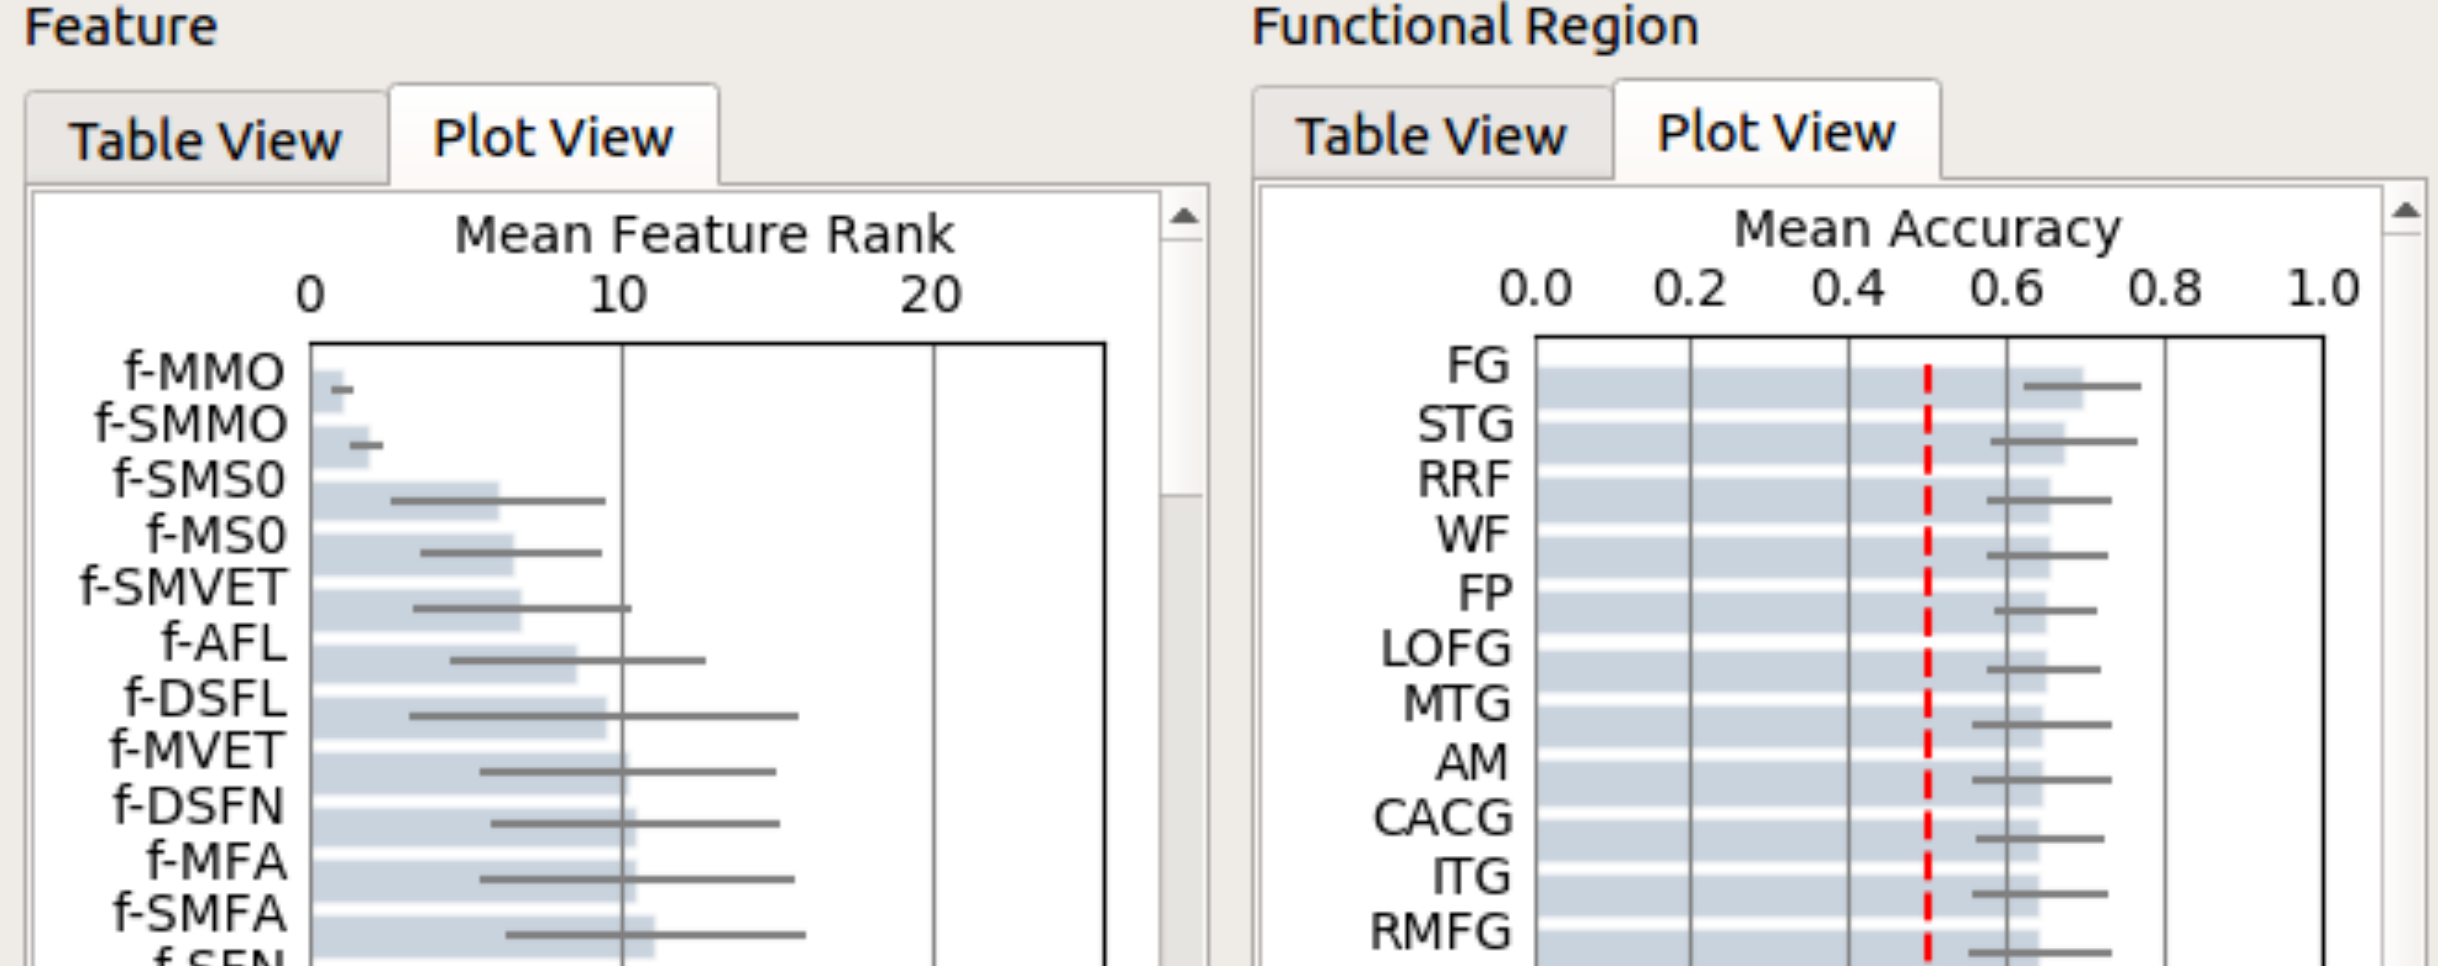
\includegraphics[width=0.85\textwidth]{images/feat.png}%
% \caption{Left)Plot view for feature exploration module. Right) Plot view for module exploration module. Blue bars show saliency score, thin gray bars show standard deviation.}
% \label{fig:regionRanks}
% \end{figure}


\subsection{Feature Exploration}
\label{sec:feature-sel}
%  Overfitting is a phenomena where a model fits the training data very well, but fails to generalize (work well on new, unseen data). Typically, the more data you have to train the model with, the better the model will generalize. Furthermore, the feature space is an important factor, and it's relation to the 

\noindent As described, high dimensional data such as ours, suffers from sensitivity to variance. One way to address this is through feature reduction. A rule of thumb is to use between $\sqrt{n}$ and $n$ features, depending on how correlated they are~\cite{hua2004optimal}. One way to reduce the feature space is dimensionality reduction. % as mentioned in~\ref{sec:feature-sel}. 
Instead, we use the given features directly, and discard less useful ones when training the predictive model. There are several possible approaches. A good one is to use statistical significance testing between each variable and the target class since these measures are familiar to scientists and fairly easy to interpret.  Downsides are that multivariate correlations are ignored, and the ranking can fluctuate widely between CV iterations. Another popular but brute force approach is recursive feature elimination, where features are eliminated one at a time if their inclusion in the feature set doesn't improve the CV estimated performance. Problems with this approach are that it doesn't provide saliency scores or rankings that can be used for exploratory analysis, it may keep many features that only slightly improve the performance of the model by random chance, and the run time can be extreme. 

Our objectives (\textbf{DG1}) require saliency scores (ideally stable ones). I.e. the saliencies shouldn't depend too much on fluctuations in the data. Ensemble based methods match these criteria well~\cite{saeys2008robust}. We use extremely random trees~\cite{geurts2006extremely}, a variant of random forests with added levels of randomization to further reduce sensitivity to variance. As mentioned, the features are scored within the CV loops $c\times(k-1)$ times. Finally, the average and standard deviation are used for prioritized VA and uncertainty awareness. In addition, we report \textit{p} values resulting from the Mann-Whitney \textit{U-test} (a non-parametric test of statistical significance) as supplemental information for additional context. The feature scores and their uncertainties populate the feature exploration module as a table view (Fig.~\ref{fig:system}\glf{C}), or a plot view (Fig.~\ref{fig:subjectsUncertainty}\glf{C}). The user can then investigate individual features by selecting them from this view. The selection is automatically linked between the other visualization view described in Sec.~\ref{sec:comparison}. 

% This allows to explore more interactive, subject comparison, as well as investigation of similarities and progression of a single subject's multiple scans over time. 

% Moreover, group level comparison of the trends of the selected features and brain region with respect to ages and genders can be seen in Fig.~\ref{fig:line_bar}. This helps the user to understand how the feature changes with age/gender and the differences between the 2 groups, as well as uncertainty awareness of each group.

\subsection{Brain Region Exploration}
\label{sec:aggregation}

\noindent As mentioned, the ML pipeline is performed for each region independently. The averages and standard deviations of the model's performance scores (Sec.~\ref{sec:subjects}) are used for salience based exploration and uncertainty awareness. As with the other exploration modules, these values can be explored in table or plot form (Fig.~\ref{fig:system}\glf{C}, Fig.~\ref{fig:subjectsUncertainty}\glf{D}).

Note that there is a hierarchical relationship between the features and regions. Each region has its own set of features with saliency scores. When a region is selected, all of the other views must update, including the feature exploration module. The fiber bundles for the region are automatically isolated in the 3D views. One design consideration is whether to compute the saliencies for all regions at once or on demand. To make the VA process interactive and support easy non-linear exploration (\textbf{DG4}), we choose to do it all at once. This causes a longer initial wait time, but that time doesn't require user interaction. The whole computation is done in parallel at a process level, with each process evaluating a separate region. When done, the visual exploration process remains uninterrupted as users can switch freely between regions without re-computing. Runtimes are reported in Sec.~\ref{sec:performance}.

%Quantitative performance results are provided in Sec.~\ref{sec:performance}.


\subsection{Classification and Across-Subject Exploration}
\label{sec:subjects}

\noindent As explained, the average predicted class probabilities and their standard deviations over all CV loops are used to guide accross-subject exploration. As mentioned, this can help support comparison and hypothesis generation (\textbf{DG3}) in a number of ways, for example: model failure (why some subjects don't fit the model, possible confounding conditions), model success (maybe an obvious case of neurodegenerative expression can be found), model ambiguity (maybe subtle expression can be found through visual analysis, or maybe different features are needed to disambiguate these subjects). In addition, we want to explore the same subjects expression across time. Changes in prediction might help guide clinical analysis and disease progression. 

For classification (to obtain probabilities that each subject has the disease), we use a linear support vector machine (SVM). This model is popular due to its high performance (including with neurological data~\cite{zhang2015detection,dinov2016predictive}), robustness against over fitting, and ability to return class probabilities (rather than just binary predictions). All of these qualities make it a good model for our domain and the objectives stated in \textbf{DG1}. 

% As the performance scores are used to rank regions, we must choose a classification performance metric.  The system reports accuracy, precision, recall, and $F_1$. We found with our data that each metric was consistently very similar in value. By default, sort by $F_1$ (which incorporates precision and recall into one score), but note that for unbalance data another metric might be preferable. 

Also, as mentioned in \textbf{DG3}, we aim to facilitate a wide range of subject-level comparative analysis through linked visualization views. First, we need to highlight/distinguish points representing multiple selected/compared subjects in each appropriate view. One complication is that there are multiple scans/time-points for each subject. In addition to highlighting and distinguishing compared subjects, we also need to associate and select between same-subject time-points and disambiguate their temporal orders. In addition, besides encoding which class the subjects belong to (disease,healthy) it's helpful to encode which class the model predicted. The subject exploration view, and these encodings are demonstrated and explained in Fig.~\ref{fig:subjectsUncertainty}.

% The ability to select individual subjects for fiber rendering based on their predicted probabilities and true values supports a useful means for exploring the variations of physical features. For example, one might expect that the more strongly effected disease brains would be predicted with a higher probability, and thus by selecting them we can see the most severe cases. By selecting lower and lower probability predictions, we can then expect to see progressively more affected subjects. Finally, we can expect that the false predictions are more likely to be outliers, and are potential indicators of bad data, for example, from imaging or processing errors, that need to be pruned out.

% As shown in Fig.~\ref{fig:subjectsUncertainty}, the probabilities and uncertainties of the subjects predicted of having PD are visualized as a sorted bar charts that include the standard deviations. The user can then investigate individual subject prediction trend and the uncertainties.

% The system supports comparison between different subjects in juxtapositioned views. The compared subjects are highlighted in the partial dependence plot and the information views, and their fiber tracts are rendered side by side in the 3D rendering views. 

% Finally, since each subject may have had their brains scanned several times over several years, when one of their scans is selected, we highlight their other scans in each of the point based information visualization views. Lines connect them while the border color of the glyph is used to indicate the currently selected time step, differentiate the different compared subjects, and help indicate the temporal order. In addition, the filled color of the glyph indicates the true class, while the shape indicates true or false prediction (circle and triangle, respectively). Additionally, we show their timelines within the fiber rendering view, with their mean values of the selected feature over time. This timeline can be used to select the subject's other scans. These views and the associated encodings are illustrated in Fig.~\ref{fig:encoding}.

% \begin{figure}[h]
% \centering
% 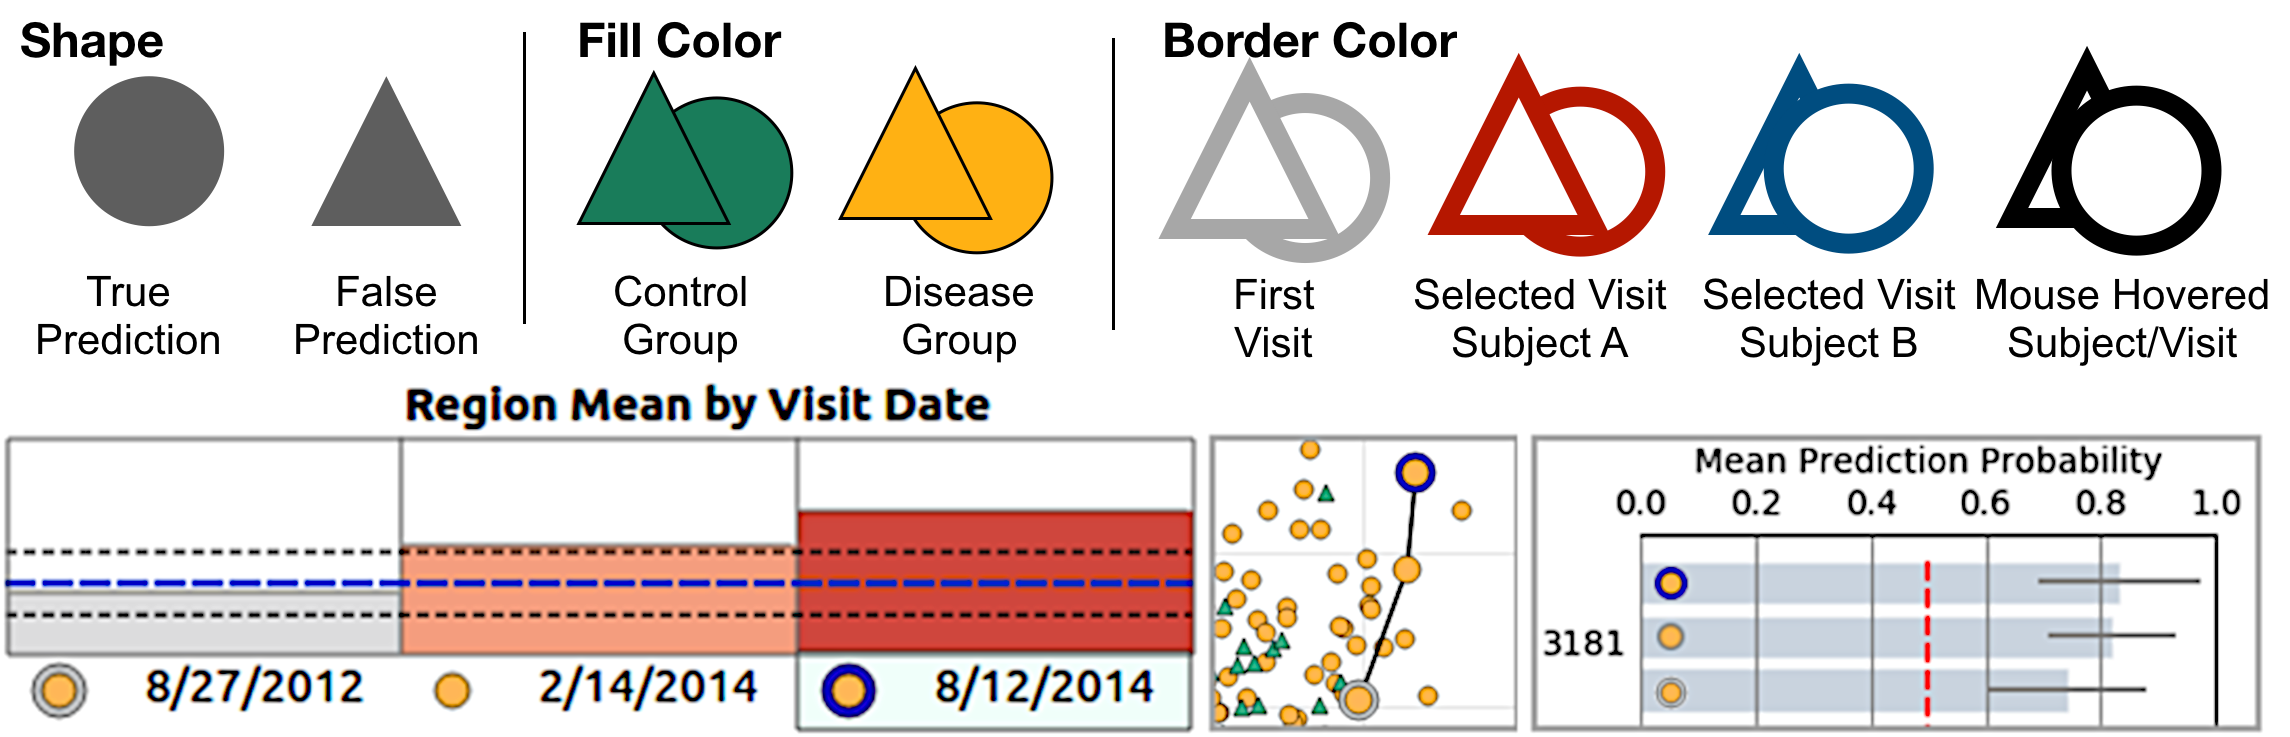
\includegraphics[width=1.0\textwidth]{images/pointEncoding.png}
% \caption{Glyph encoding. Shape encodes predicted class, fill color encodes true class, and the border distinguishes between pairs of selected subjects, and the temporal order of their different time-points (in conjunction with connecting lines for scatter plot views).}
% \label{fig:encoding}
% \end{figure}

\begin{figure}[tb]
\centering
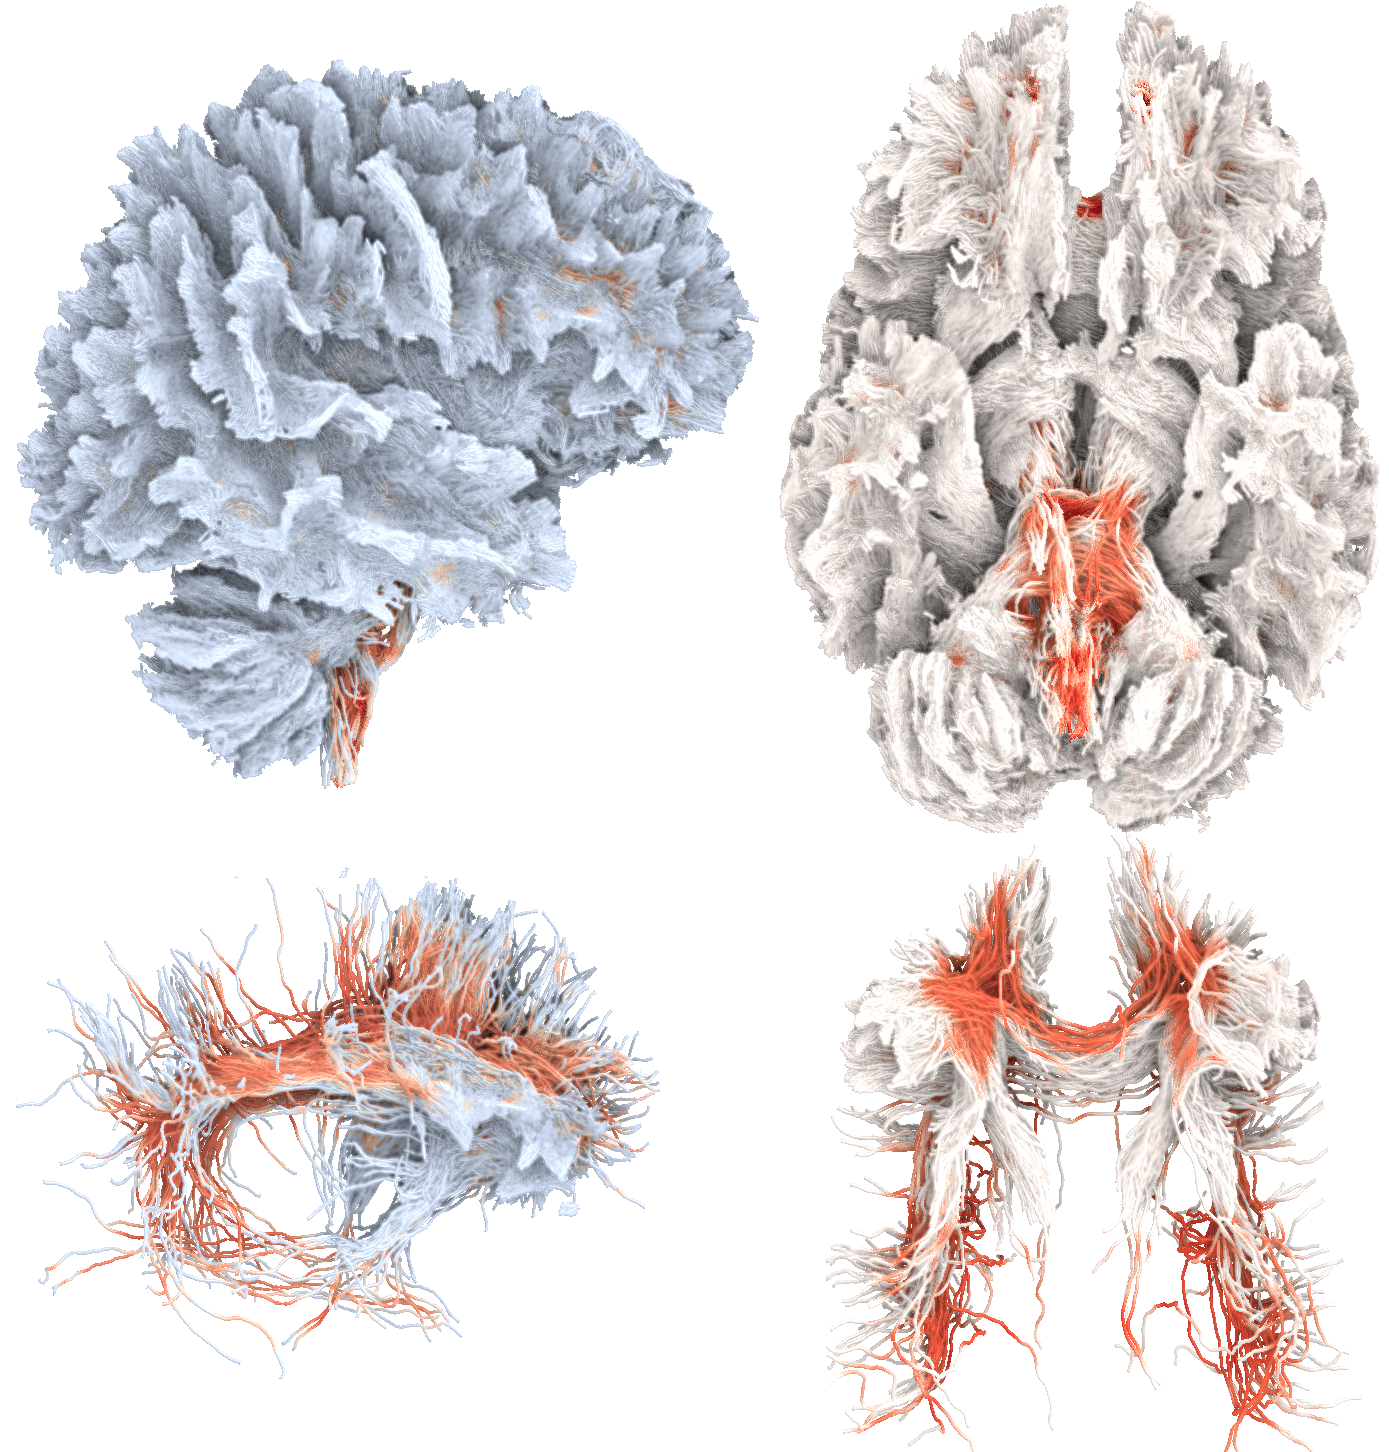
\includegraphics[width=0.99\textwidth]{rendering2.png}
\caption{Each column shows the whole brain and one bundle at the same orientation. SSAO rendering achieves a shadow effect that enhances spatial perception. (Left) diverging colors encode difference from the mean of the healthy group. (right) direct color mapping.}
\label{fig:rendering}
\end{figure}

\begin{figure*}[t]
\centering
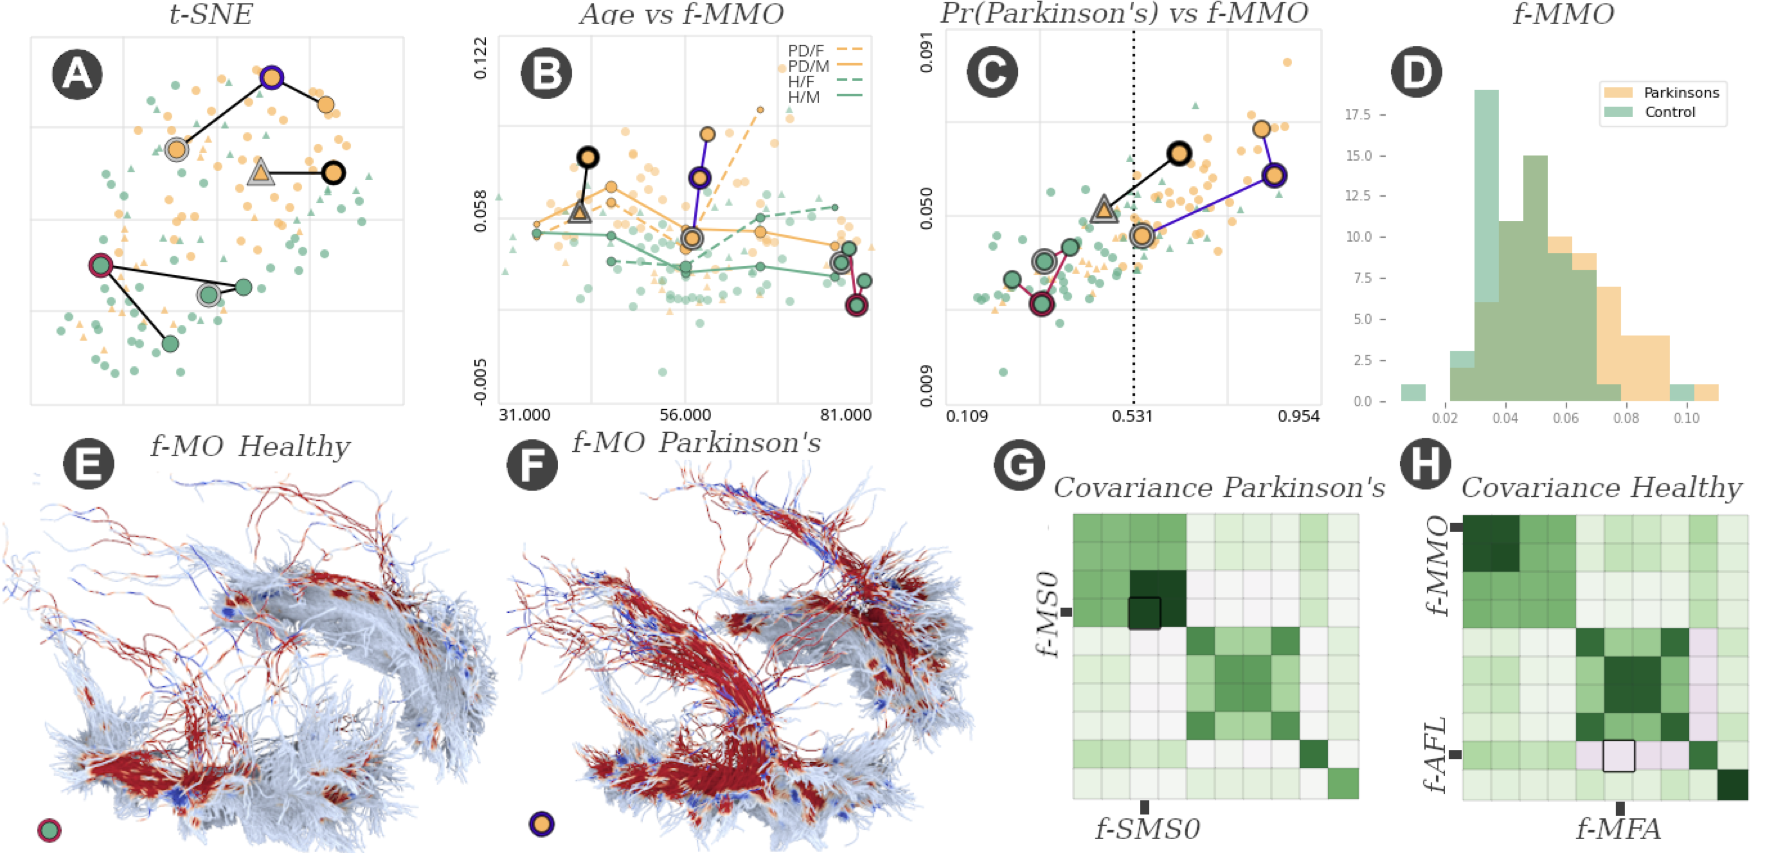
\includegraphics[width=0.99\textwidth]{images/comparisonV3labeled.png}
\caption{Visual comparisons in linked views (encodings are explained in Fig.~\ref{fig:subjectsUncertainty}). \glf{A} t-SNE plot using top 10 features with compared subjects highlighted. This view hints at multivariate similarity and ``community" structure.
\glf{B} Group trends in age vs mean mode of anisotropy (mean MO) in the fusiform region (f-MMO); dotted lines: female, solid lines: male, orange: PD, green: HC. \glf{C} Estimated probability of Parkinson's vs f-MMO. Dotted line shows the discrimination threshold (0.5). From this plot you can gain insight into the contribution of the salient feature to the classification model. You can then use the mouse to pick out subjects within the plot for various analysis directions. For example, select subjects that don't fit the group trend (e.g. correctly predicted PD subjects with low f-MMO), and then evaluate those subject's other features to better understand why the model predicted their class. \glf{D} Comparison of the distributions in f-MMO by group. This is a high level group comparison that gives instant insight into the group difference, and may also give insight into the statistical quality of the data. \glf{E},\glf{F} the fusiform fibers colored by the dis-aggregated MO values for the compared subjects The HC (left) and PD subject (right) are identified in the linked views by the green circle with red border, and orange circle with blue border respectively. \glf{G},\glf{H} Comparisons of the covariance for the top 10 features for the HC and the PD group respectively. Some interesting observations are pointed out: f-MMO (the salient feature) has higher variance in the Parkinson's group, and in bother groups is correlated positively with several other features. Second, a negative correlation between average fusiform fiber length (f-AFL) and mean fusiform fractional anisotropy (f-MFA) emerges for the Parkinson's group. Thirdly, there is a reduced overall in many of the features in the PD group compared with the healthy group. In the full user interface, the highlighted subjects are also shown in the time-point selection module, parallel coordinates view, and the subject exploration module as shown in Fig.~\ref{fig:system}, and Fig.~\ref{fig:subjectsUncertainty}.}
\label{fig:infovis}
\end{figure*}


\subsection{Fiber Rendering}
\label{sec:rendering}

\noindent The brain fibers are rendered (Fig.~\ref{fig:rendering}) as path tubes with screen space ambient occlusion (SSAO). This produces a high quality visualization with enhanced spatial perception that better shows fiber structure~\cite{mittring2007finding, eichelbaum2013lineao}. The path tubes are constructed on the fly through the GPU rendering pipeline in the geometry shader. This allows the pathtubes to be constructed and rendered quickly, with an interactively adjustable radius, and without additional memory overhead. The subjects, regions, and features (selected from their respective exploration modules) automatically determine which fibers are rendered, and which variables are used for color mapping.  User selected rendering options include: contrastive color mapping (which uses the difference from the mean value of the healthy group in order to emphasize anomaly), log scaling (which can better reflect subtle differences), and pathtube radius (which can help reduce or increase detail). These design decisions reflect \textbf{DG2} by providing a high quality visualize of fiber-microstructure with interactive frame-rates for large sets of brain fibers. 


\begin{figure*}[t!]
\centering
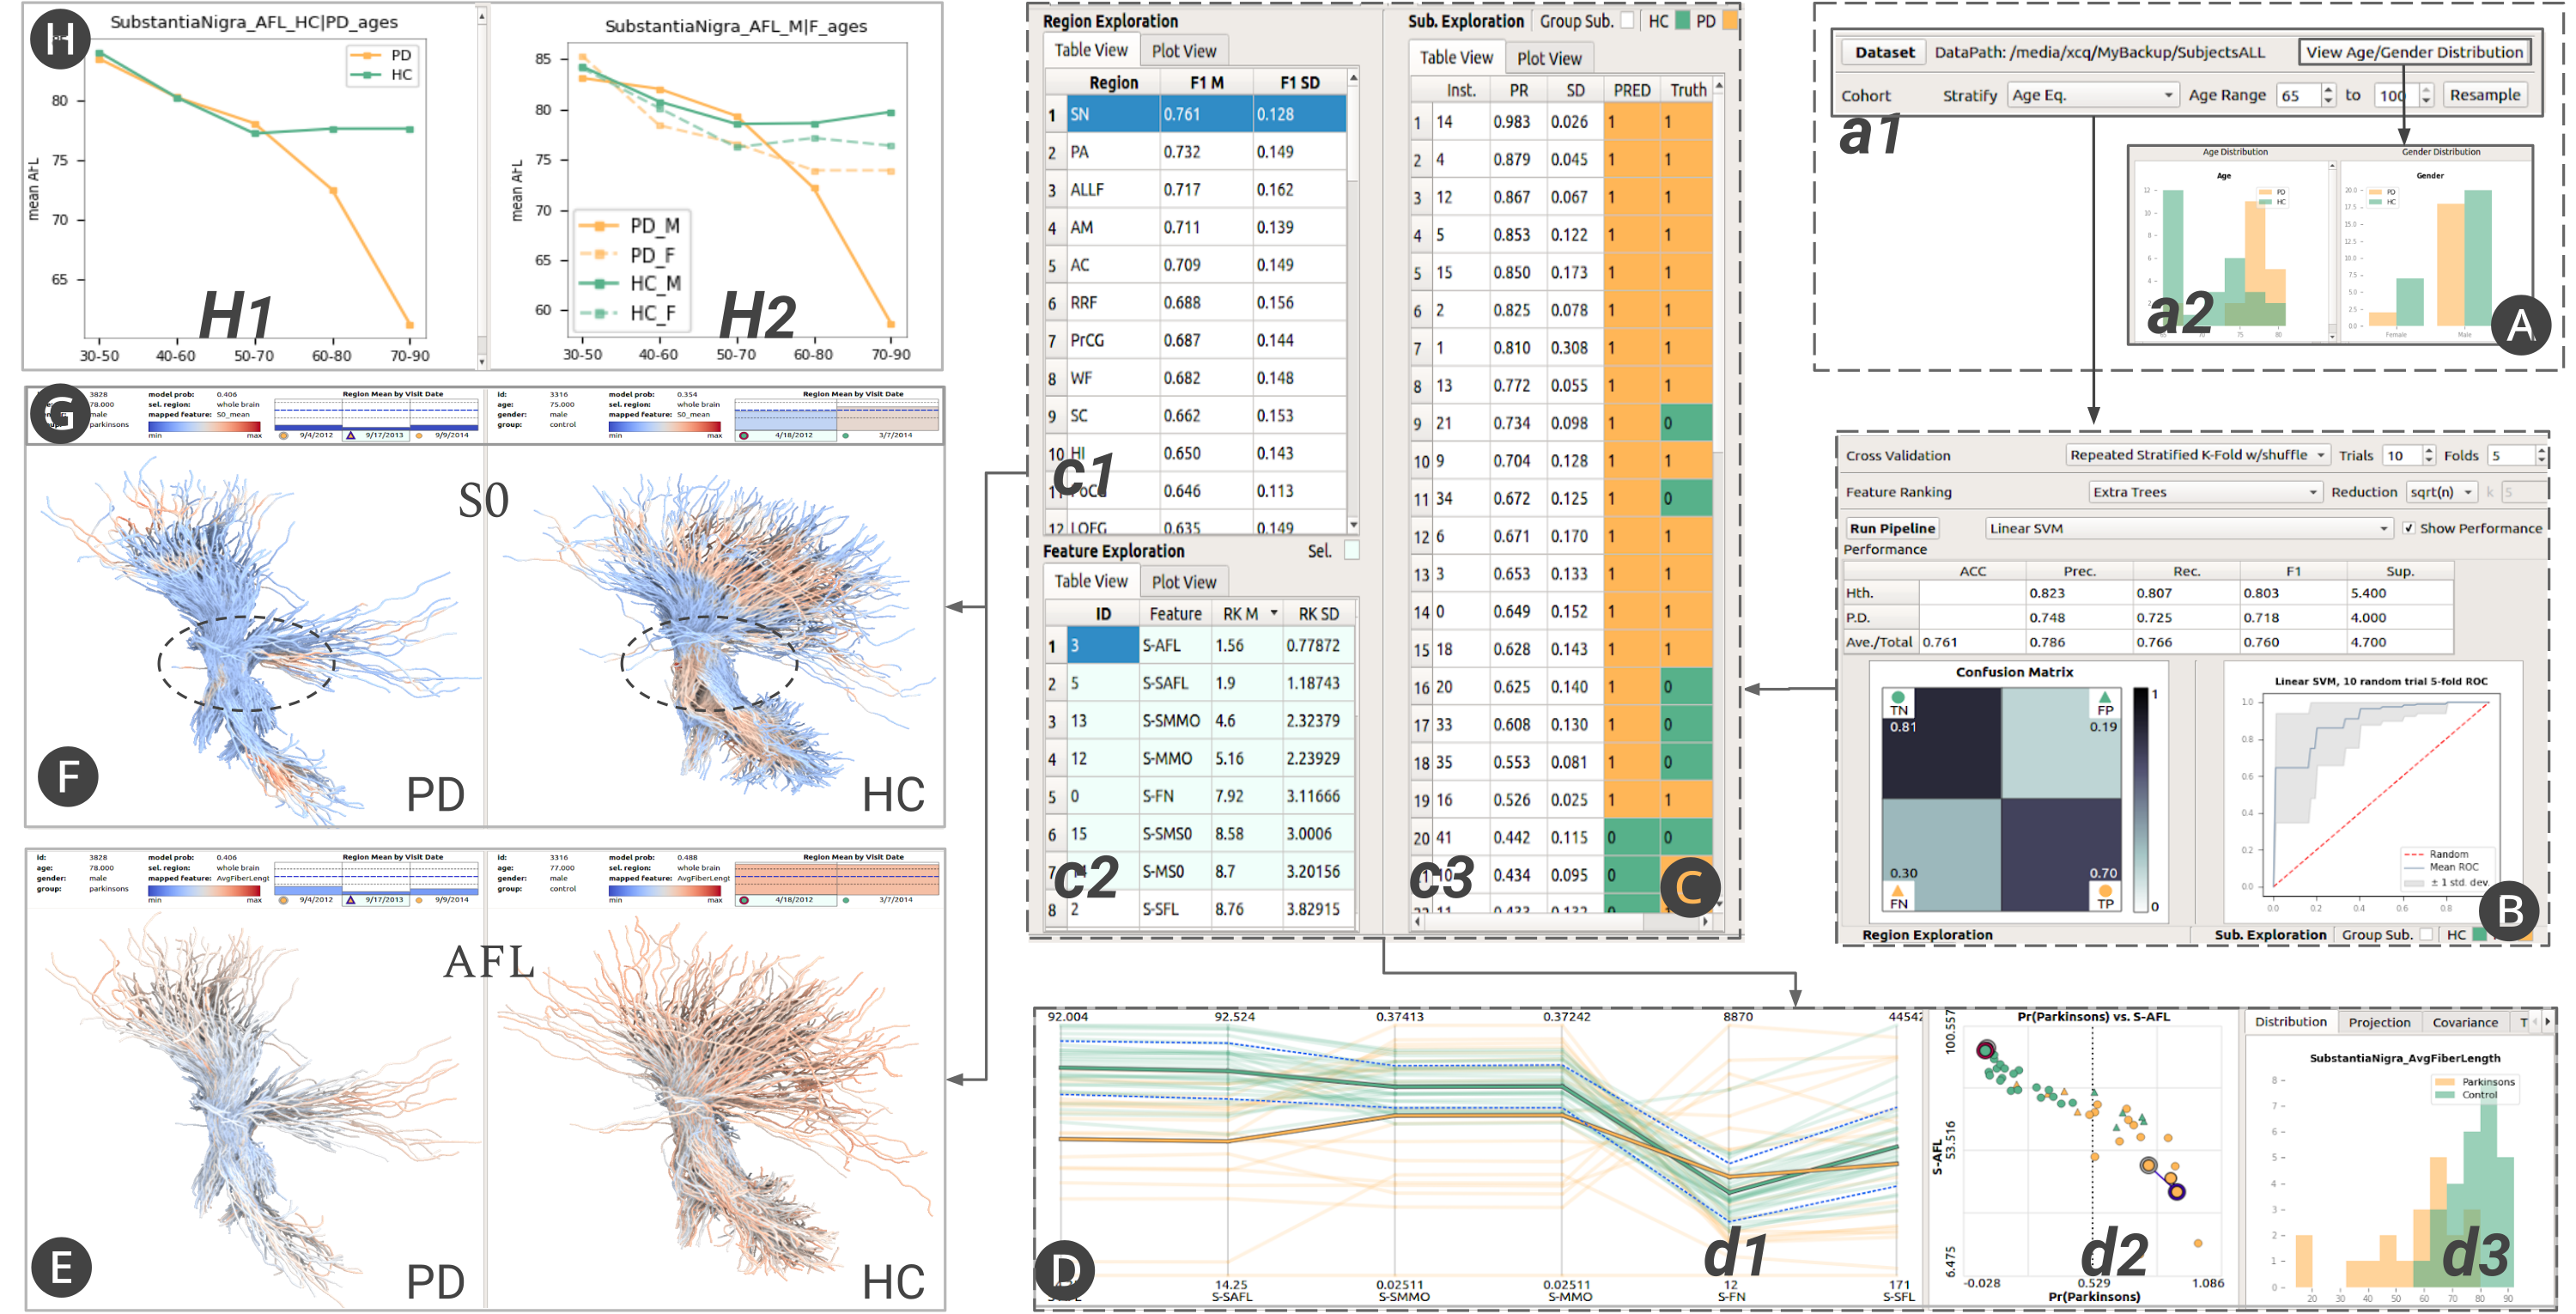
\includegraphics[width=0.98\textwidth]{images/SNSteps_v5.png}%
\caption{ Data selection module \glf{A}, entering an age range from \textbf{\textit{a1}} and displaying the distribution in \textbf{\textit{a2}}. ML module \glf{B}. users can run a ML algorithm with input parameters. Prediction results module \glf{C}. Brain regions \textbf{\textit{c1}}, features \textbf{\textit{c2}}, and subjects \textbf{\textit{c3}} were sorted in the table. Information visualization module \glf{D}. parallel coordinate \textbf{\textit{d1}}, partial dependence plot \textbf{\textit{d2}}, and bar chart \textbf{\textit{d3}} were used to show the distributions of the features and subjects. 3D rendering module \glf{E} and \glf{F}. Brain fibers were rendered in the juxta-positioned 3D rendering views for visual comparison with timeline views \glf{G}  of the selected subjects. Group trends plotting module \glf{H} ( trends with age \textbf{\textit{H1}} and trends with gender \textbf{\textit{H2}} ).}
\label{fig:SNSteps}
\end{figure*}


\subsection{Comparative Analysis}
\label{sec:comparison}

\noindent To support \textbf{DG3} we include a range of linked information visualization views that support a range of comparative modes for analysis. Besides the exploration modules, this includes: a histogram view, parallel coordinates view, scatter plot view, trend view, dimensionality reduction view, covariance matrix view, and subject time-point view. The views are linked with the exploration modules as shown in Fig.~\ref{fig:subjectsUncertainty}. The main aspects which are novel, are how they are customized to support the different modes of comparison for our application. We demonstrate by example in Fig.~\ref{fig:infovis}, and in the case studies in Sec.~\ref{sec:cases}. We reserve the rest of this section for some additional noteworthy details.  

Both covariance matrices and parallel coordinates can benefit from sorting to better highlight patterns~\cite{1382895}; in our case we apply hierarchical clustering to group correlated variables using the Louvain community detection algorithm~\cite{donetti2004detecting}. The same sorted order is applied to both views to assist the mental map~\cite{1215004}. The user can also switch from a covariance matrix to a correlation matrix.

Besides the information visualization views, the fiber views also incorporate design elements to facilitate comparison. First, the color map is scaled to be constant over all of visualized brains; after cohort selection, a global value range must be gathered over all subjects. Second, an option supports coloring the fibers by difference from the mean of the healthy control (HC) group. This supports comparison of the individuals against the HC, which may better emphasize important differences. The cameras between these views can also be linked so that they pan, rotate and zoom together. 

%One additional note, is that 
Uncertainty plays a major role in the workflows supported by our system. This begins with the overall model performance view (Fig.~\ref{fig:system} \clc{B}), which includes a receiver operating characteristics (ROC) curve. The ROC curve is used to assess the effect of prediction threshold on performance characteristics. In our case, we also highlight the variance of this curve over all CV trials, which is useful for assessing the overall sensitivity of the model to the training data. This is an important measure of uncertainty to consider during further comparative analysis. Once the user has made those assessments, they can collapse the view, to expand the sizes of the exploration module views. The variance each of the saliency measures is also included in the exploration modules (tables/plots) to make further assessment while exploring. These are important references to make while doing comparison, in order to avoid overconfidence and false insight.


\section{Results}
\label{sec:cases}
% \begin{figure*}[!ht]
% \centering
% 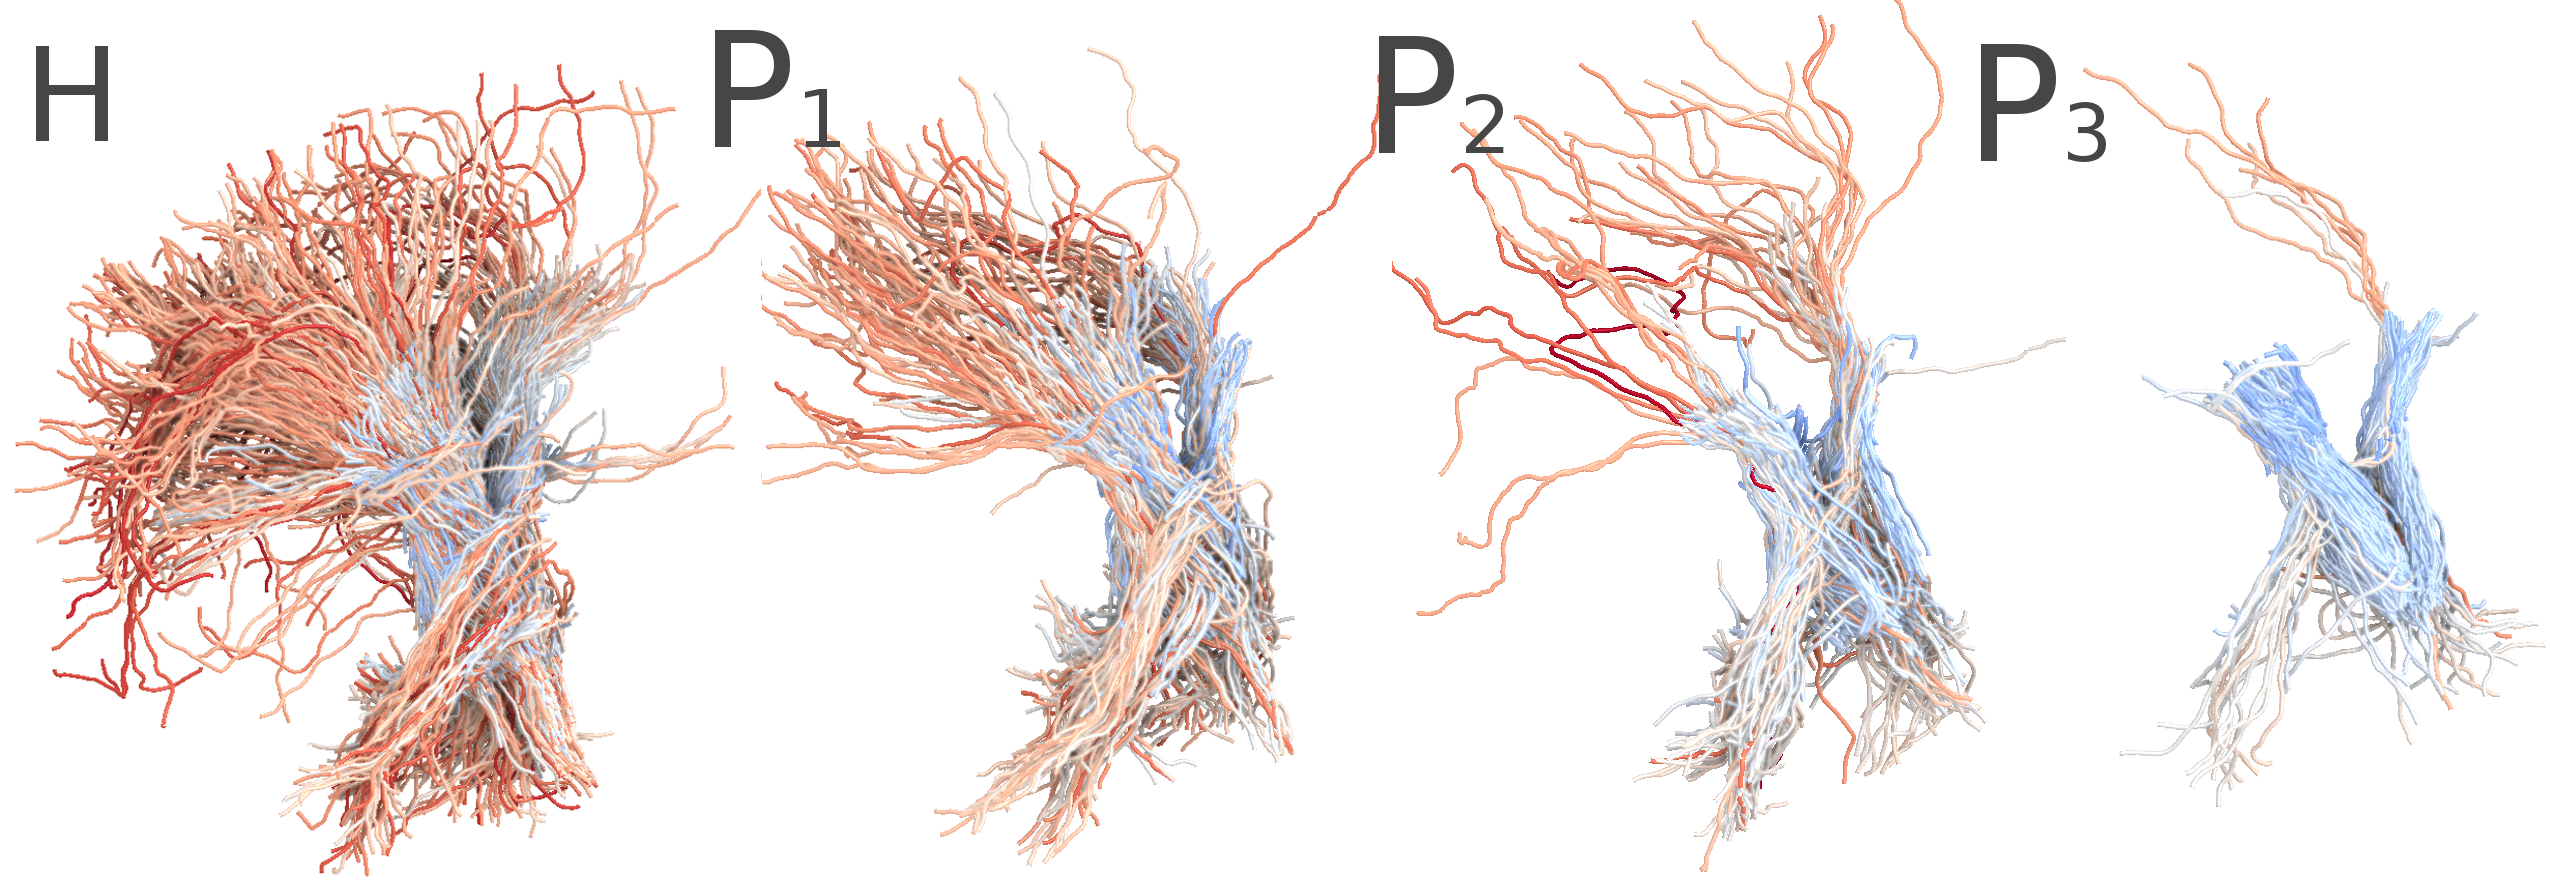
\includegraphics[width=1.0\textwidth]{degeneration.png}
% \caption{The type and severity of fiber loss found among some of the disease group subjects. On the left $(H)$ shows a typical full intact region from a control group subject. $P_1$ through $P_2$ show progressively worse cases of fiber loss. This is a characteristic observed within the disease group, but the severity depicted in $P_2$ and $P_3$ were quite rare, and some apparent loss was observed within control group subjects as well.}
% \label{fig:loss}
% \end{figure*}

\noindent % Each of 
Our studies are based on DTI images and %reconstructed 
derived fiber tracts of Parkinson's and Control groups obtained from the 
%research 
database of PPMI~\cite{marek2011parkinson}. Five experts with different professional backgrounds are involved in our case studies and/or the evaluation of our system. The first (E1) is a radiologist who focuses on 3D visualization of medical images and brain disease analysis of high-resolution brain fiber tracts. The second (E2) is a neurologist who specializes in treating motor disorders such as stroke, PD, and epilepsy. The third (E3) is a physician of neurology, mainly engaged in cerebral stroke and Alzheimer's disease clinical/research work. The fourth (E4) is a neuroscientist with expertise in statistical analysis, tractography, and neurodegenerative disease. The fifth (E5) is a neurologist at a children’s hospital specializing in diagnosis and treatment of congenital nervous system malformations, and voxel-based morphometry (VBM) analysis of Hunting-ton’s disease. E1,E2, and E3 were involved in the case studies, while E4 and E5 provided qualitative feedback. One challenge in evaluating our system is that none of the consulted domain scientists are an expert in all 3 areas (brain fibers, Parkinson's disease, and machine learning). We should also point out that we are not drawing scientific conclusions about Parkinson's disease in our case studies, but are instead focused on demonstrating the usage of our system and the types of insights it can provide.

% \begin{figure}[!t]
% \centering
% 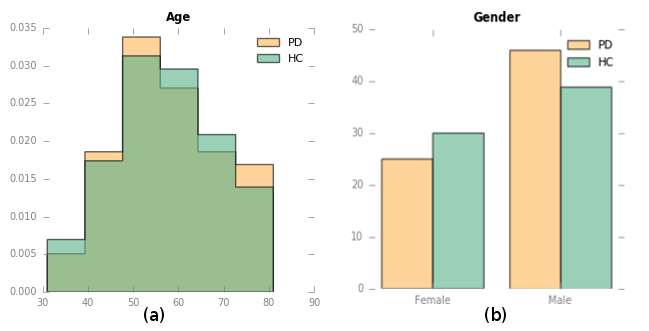
\includegraphics[width=1\textwidth]{images/Demographic.png}
% \caption{Demographics of the dataset. The age distribution (a). The two sets of data have similar age distributions. The gender distribution (b). In both disease group and HC, the amount of male data is more than that of female.("The incidence of Parkinson’s disease is low before
% the age of 50 years, but it increases rapidly with age,peaking in most studies at around 80 years, probably
% because of underdiagnosis with increasing age" -- copy from \cite{ASCHERIO20161257})}
% \label{fig:demographic}
% \end{figure}



\subsection{Data Acquisition and Processing}

\noindent MRI parameters, such as gradient direction, b-value, and voxel resolution, have a crucial impact on the scalar measurements that are used for clinical study. To prevent errors, the MRI images provided by PPMI, were collected based on standardized and strict acquisition protocols developed by the steering committee on 3T Siemens scanners.

Each subject includes DTI and T1-weighted images. For each DTI image, a 2D echo-planar DTI sequence was acquired with the following parameters: TR = \SI{900}{ms}, TE = \SI{88}{ms}, Image matrix $= 116\times116\times72$ and voxel resolution $ = 1.98\times1.98\times2$\SI{}{mm^3}, 64 gradient volumes (b = \SI{1,000}{s/mm^2}), and one non-gradient volume (b = \SI{0}{s/mm^2}). The acquisition parameters for T1-weighted images are as follows: TR = \SI{2,300}{ms}, TE = \SI{2.98}{ms}, Image matrix $= 160\times240\times256$ and voxel resolution = $ 1\times1\times1$\SI{}{mm^3}.

Both the DTI and T1-weighted images require preprocessing, since a variety of issues affect fiber tracking results, such as intensity loss, blurring, gradient distortion, and inhomogeneities in the applied magnetic field. Correction is required to accurately estimate fiber orientation and achieve alignment from DTI to T1-weighted images, which would affect MRI coregistration (intra-subject registration) and cause great deviation in the extracted fibers from Regions of Interest (ROI).

% All DTI and T1-weighted images were converted from the Digital Image and Communications in Medicine (DICOM) format to Neuroimaging Informatics Technology Initiative (NIFTI) format. 

For our study, DTI images were processed using MRtrix3~\cite{mrtrix3}. We first denoised each DTI, and then performed Echo-planar Image/fieldmap correction, eddy current correction, and head motion correction; finally, we performed B1 field inhomogeneity correction for the DWI volume series. The preprocessing procedures for T1-weighted images are based on FreeSurfer~\cite{freesurfer}, including motion and non-uniformity correction. T1-weighted image volumes were registered to the DWI images using FSL~\cite{fsl}. % 5.0.10~\cite{fsl}.

Brain fiber tractography was performed using a state of the art framework~\cite{SMITH20121924}, which can reconstruct neuronal axons and retain biological accuracy. This framework was also used to generate the tract-based, and tensor-based features. 

We then used our system to analyze the data. Our system applies an ML pipeline that includes feature selection/reduction and classification. All stages were done using cross validation as described in
Section~\ref{sec:CrossValidation}. Since the overall performance depends on the data set and specific sets of selected features (which vary between case study), we provide the classifier's cross validation performance scores separately in the respective subsections.

% \textcolor{blue}{After feature extraction of the fiber tracts (section \ref{sec:extraction}), the dataset used for machine learning would have high-dimensional features and each of the subjects would be labeled PD or HC. After that, $k$-fold cross validation was used to split the dataset into training sets and test sets (section \ref{sec:CrossValidation}). Then we can train the predictive model and evaluate the performance.}

\subsection{Disease Background}

\noindent PD is a neurodegenerative disorder characterized by loss of dopamine neurons in the substantia nigra (SN) brain region~\cite{prakash2012asymmetrical}. The dopaminergic function of the nigrostriatal pathway reduces with the depletion of these neurons, as well as the neural fibers that link the SN to other subcortical regions, such as putamen and caudate \cite{zhang2015diffusion}. Each region in the mid brain is affected based on the anatomical correlation with SN and the severity of the region reflected by the functional relationship with SN. %\cite{zeighami2015network}. 
It is recognized to be a brain-wide neurodegenerative process that spreads up from brainstem into the cortex, as originally suggested by Braak.etc~\cite{yau2018network}. %Significant effects were also observed in the whole Parkinson's disease brain with spatial distribution of quantitative susceptibility mapping (QSM) \cite{atkinson2017diffusion}. 
PD also increases rapidly with age, with low incidence before 50, and most cases found around 80~\cite{ASCHERIO20161257}. Once the fibers are detected by tractography, it is useful to assess the diagnosis with the brain fiber pathways. 

% \begin{figure*}[t]
% \centering
% 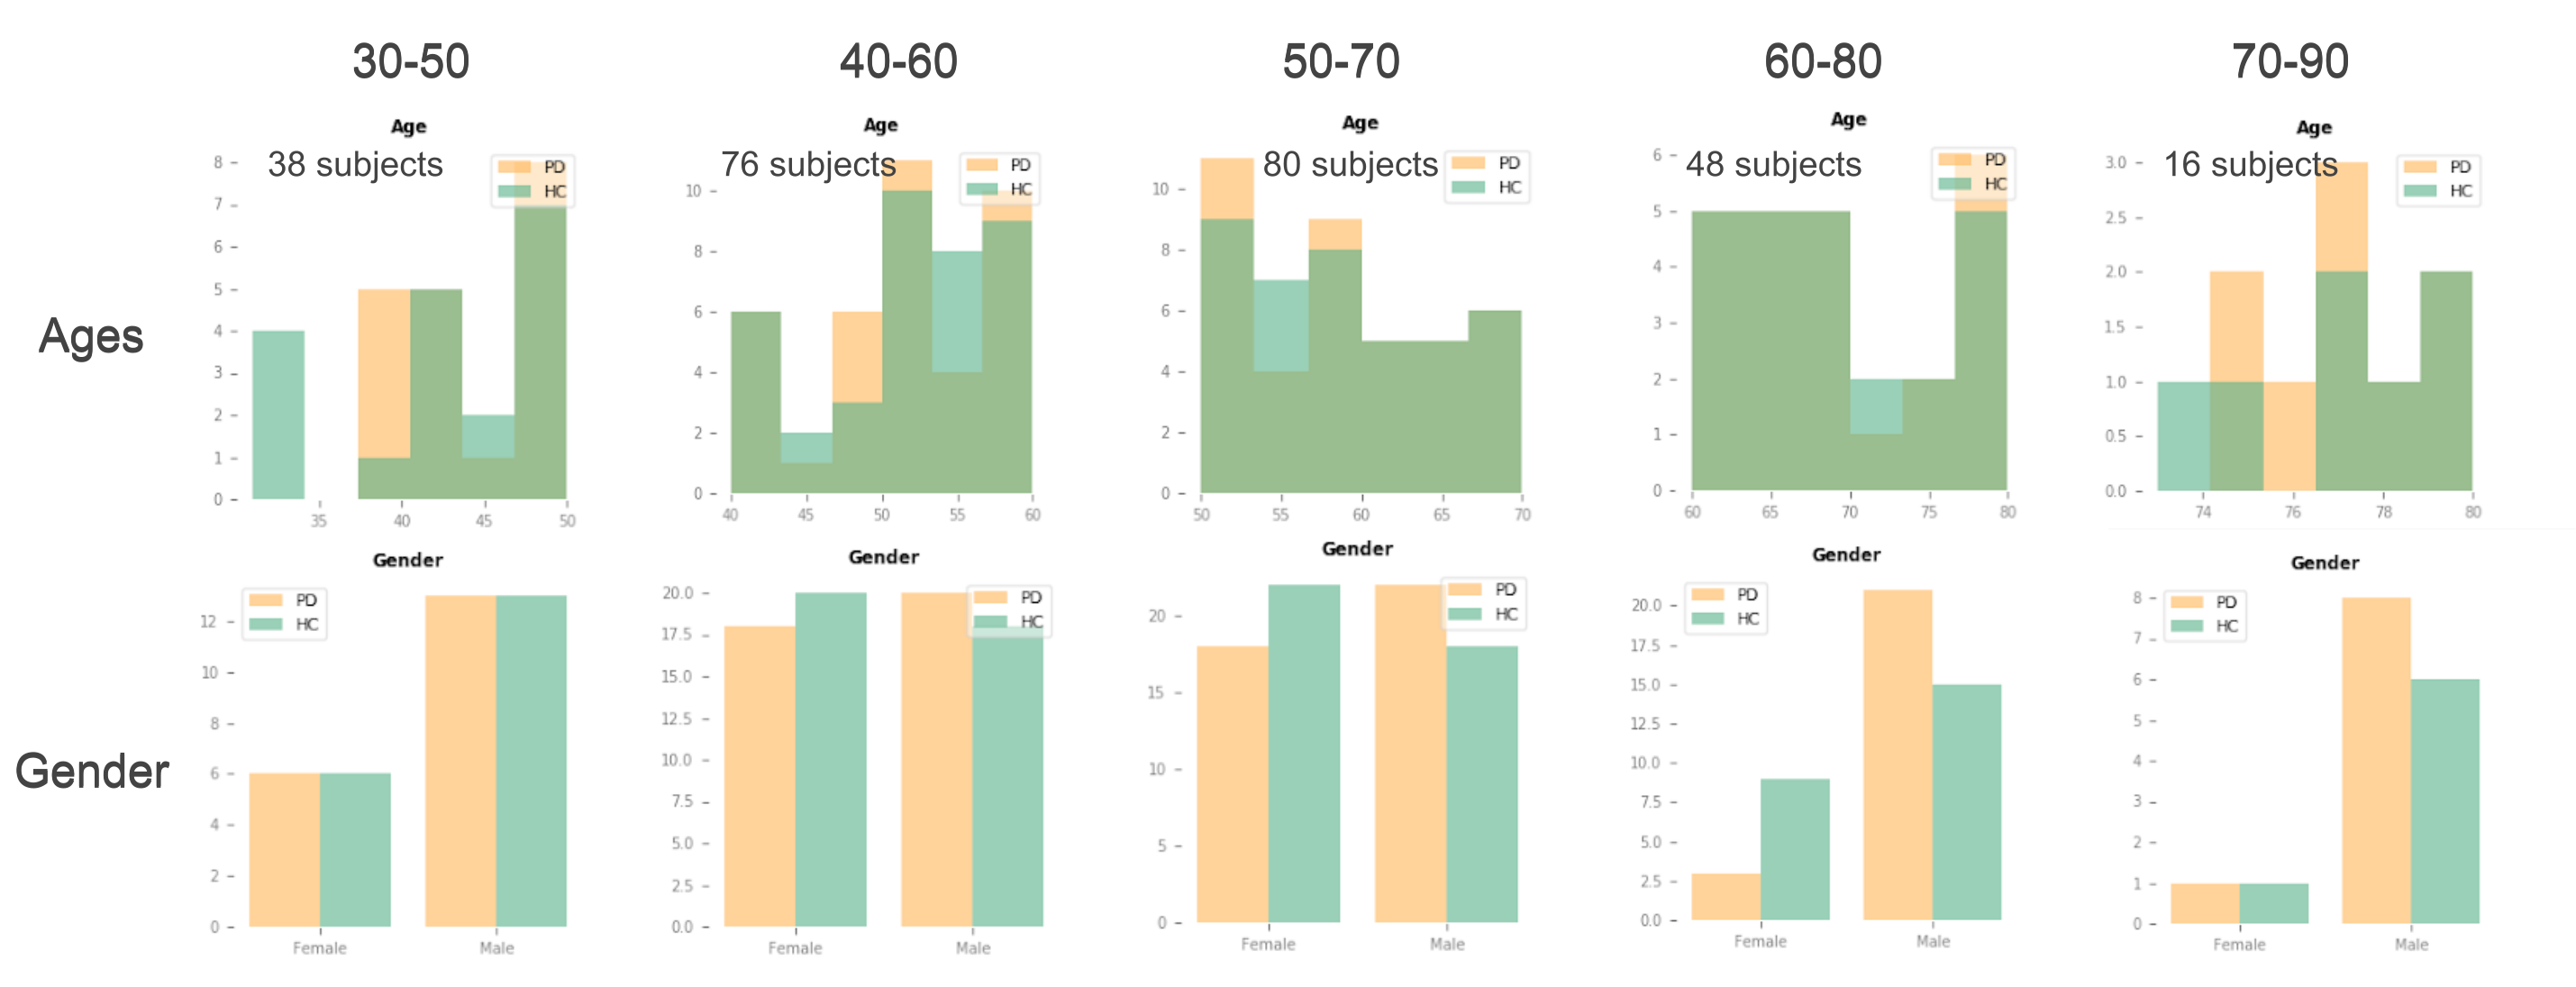
\includegraphics[width=0.85\textwidth]{images/groupsDemographics.png}
% \caption{Age and gender distributions of 5 subgroups, which have been divided by ages with 20 as the step size. The first row shows the age distributions of each subgroup, while the second row shows gender distributions. 
% In the age distribution histograms, the overlap part of the HC and disease group is drawn in light green.}
% \label{fig:groupDemographics}
% \end{figure*}



% \begin{figure*}[t]
% \centering
% 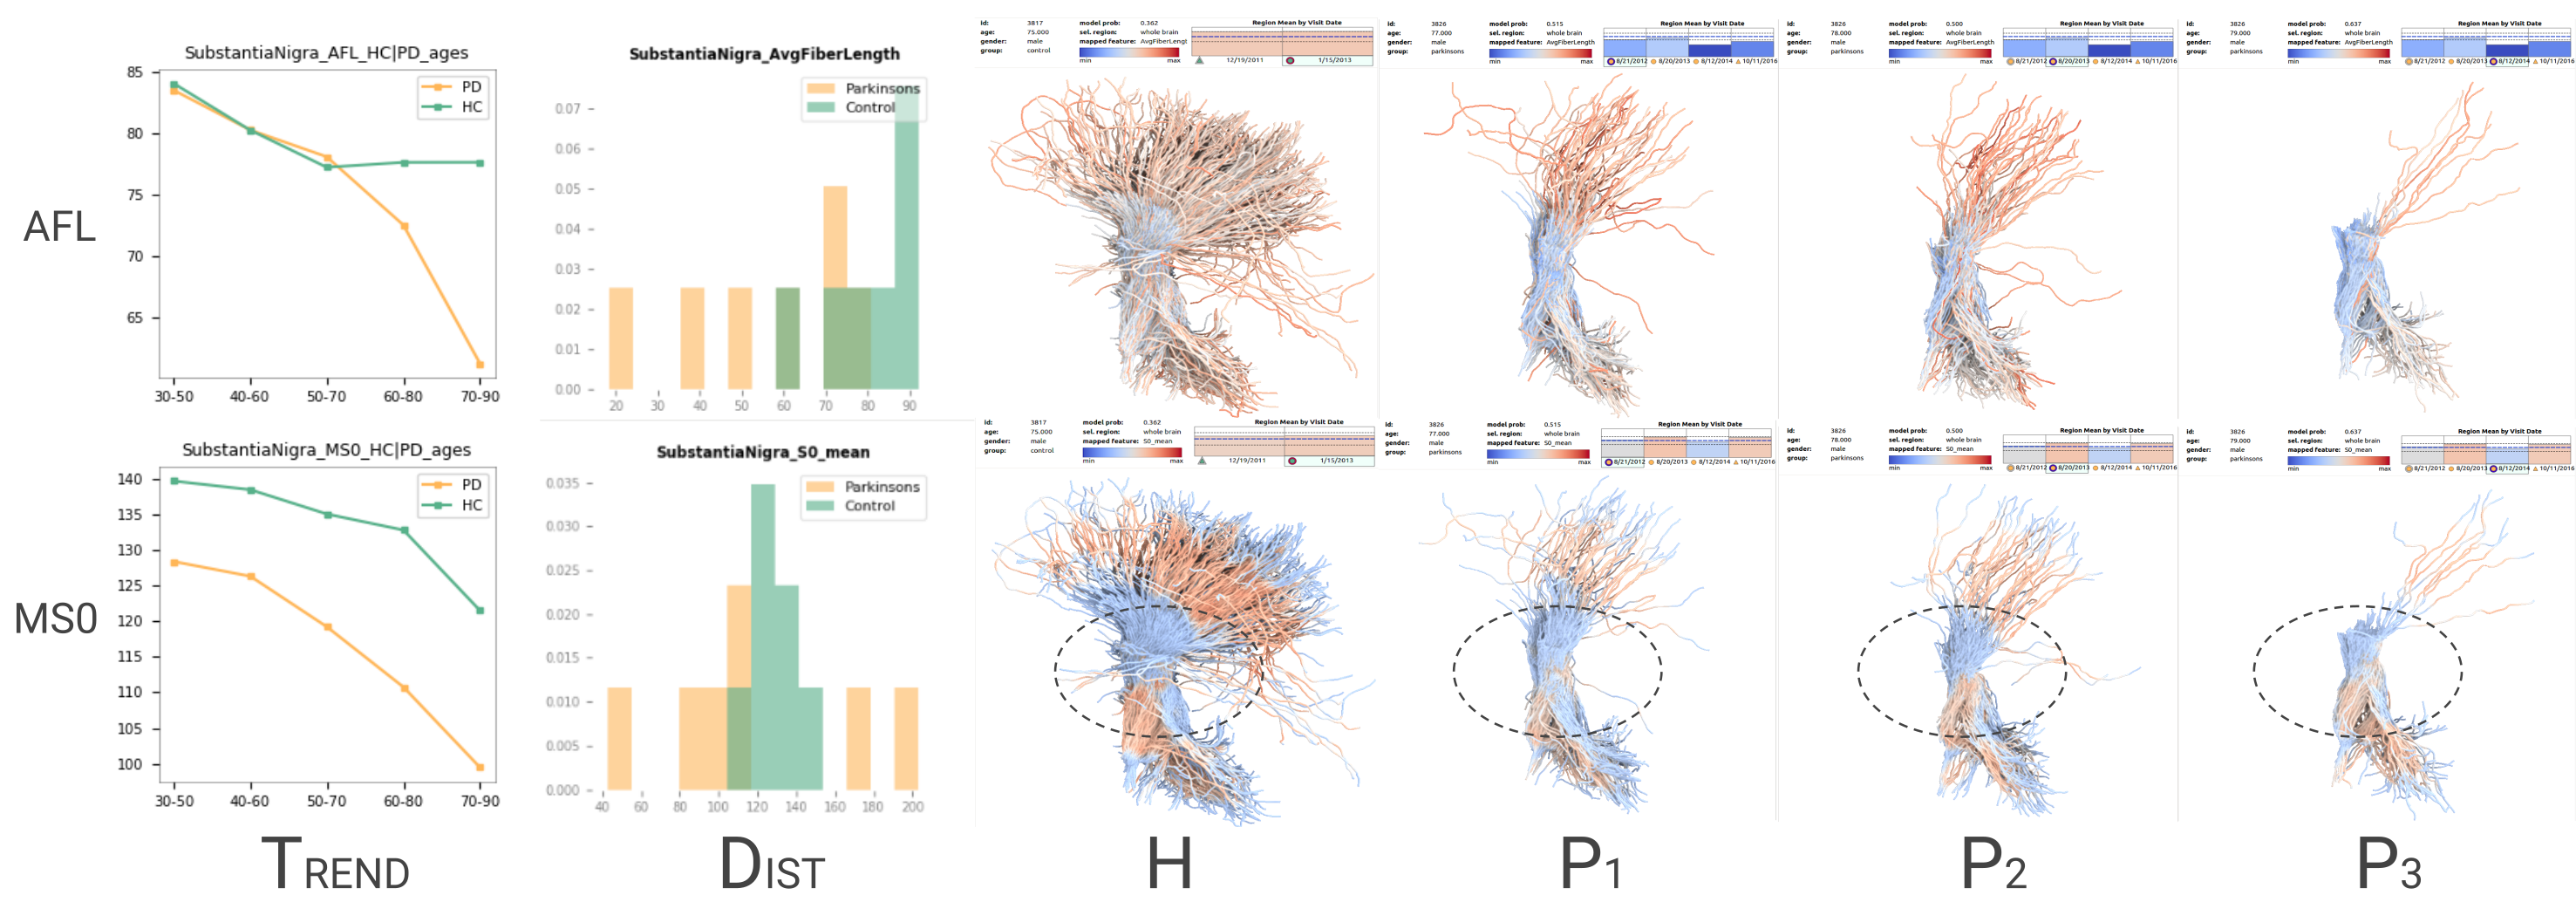
\includegraphics[width=0.85\textwidth]{images/SNcase_v3.png}
% \caption{ PD effects in nigrostriatal fibers and tensor features within the elderly group. The $Trend$ column shows the feature changes in different ages. The $Trend$ column shows the views for comparing the groups' distributions of the selected feature. $H$ column shows the nigrostriatal fibers of a subject from the HC, while $P1$ to $P3$ show the nigrostriatal fibers of a subject in different years. The two rows show two different feature performance on PD. $AFL$ is short for average fiber length, and $MS0$ indicates mean value of raw T2 signal with no diffusion weighting.}
% \label{fig:SNcase}
% \end{figure*}
%\textbf{D}\text{\small{IST}}

% \subsection{Case Study 1: Exploration of Parkinson's Disease with the Nigrostriatal ROI}

\subsection{Study 1: Exploration of PD with the Nigrostriatal ROI} %(a

\begin{figure*}[t]
\centering
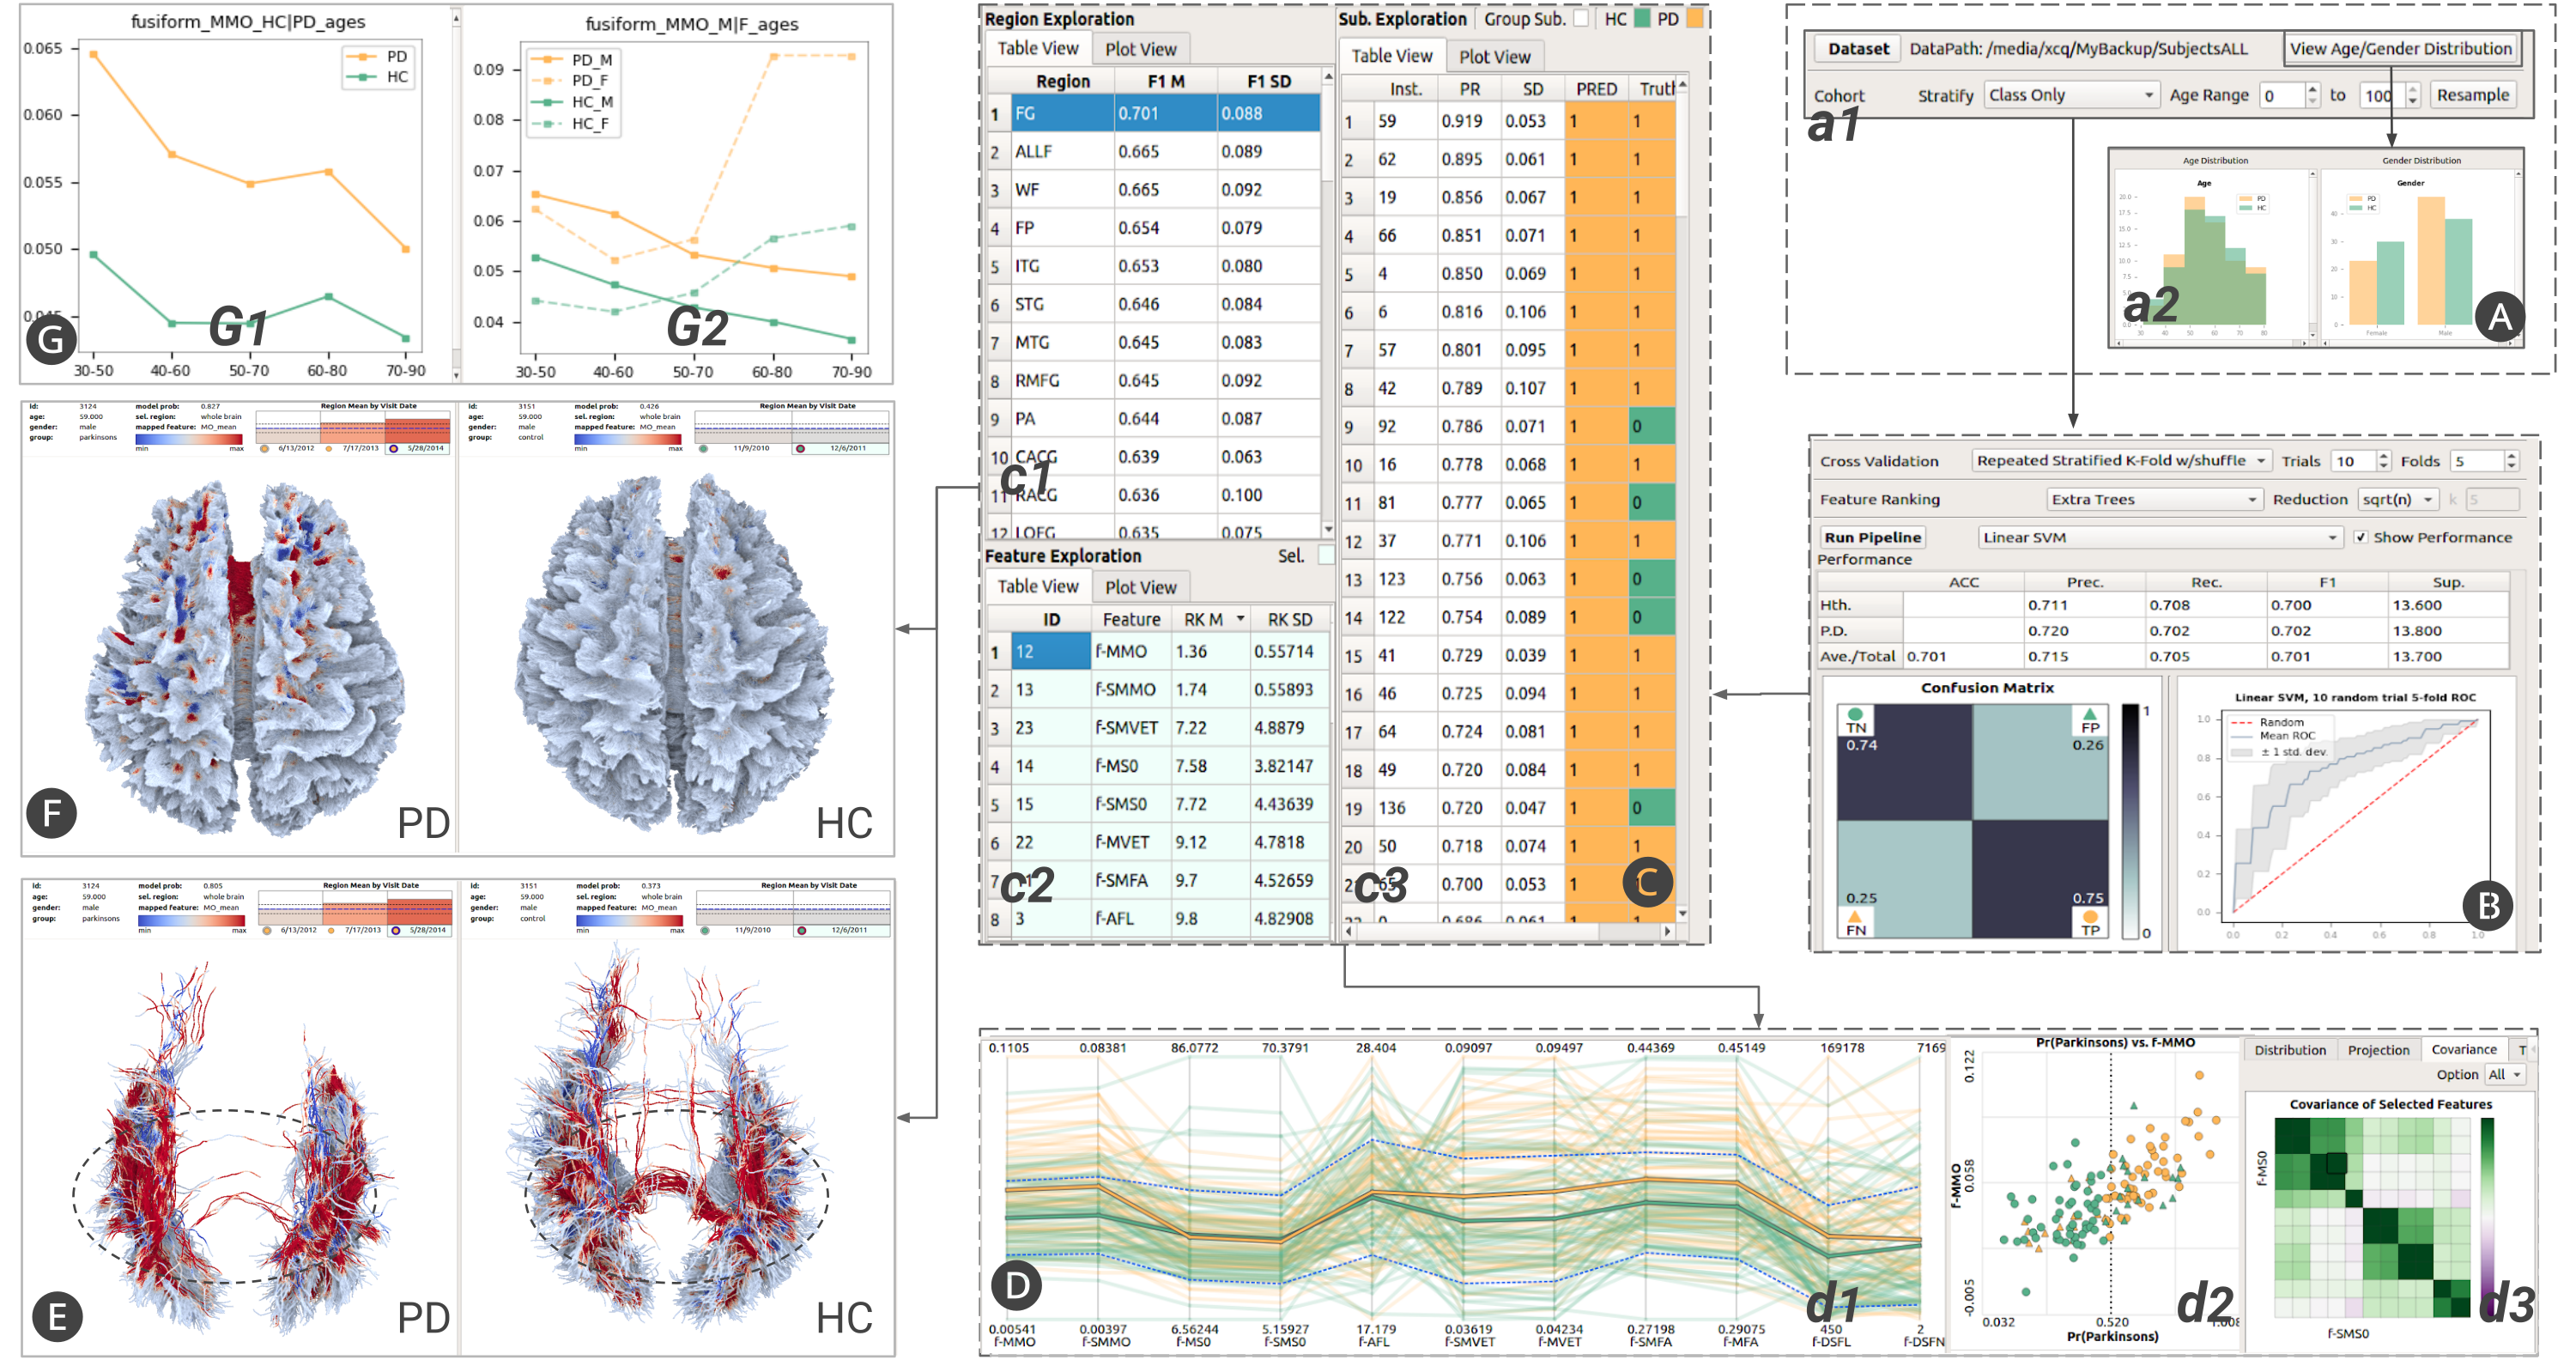
\includegraphics[width=0.99\textwidth]{images/fusiformSteps_v5.png}
\caption{ Data selection module \glf{A}, entering an age range from \textbf{\textit{a1}} and displaying the distribution in \textbf{\textit{a2}}. ML module \glf{B}. users can run ML algorithm with input parameters. Prediction results module \glf{C}. Brain regions \textbf{\textit{c1}}, features \textbf{\textit{c2}}, and subjects \textbf{\textit{c3}} were sorted in the table. Information visualization module \glf{D}. parallel coordinate \textbf{\textit{d1}}, partial dependence plot \textbf{\textit{d2}}, and covariance matrix view \textbf{\textit{d3}} were used to show the distributions and relations of the features and subjects. 3D rendering module \glf{E} and \glf{F}. Brain fibers were rendered in the juxta-positioned 3D rendering views for visual comparison with timeline views of the selected subjects. Group trends plotting module \glf{G} ( trends with age \textbf{\textit{G1}} and trends with gender \textbf{\textit{G2}}).}
\label{fig:fusformSteps}
\end{figure*}

\noindent Based on the disease background,
% that PD is histopathologically characterized by the loss of dopamine neurons in the substantia nigra pars compacta, 
we decide to explore fiber bundles with streamlines starting from the SN region; our focus is on trends with age, and spatial feature patterns from older subgroups (where significant symptoms have been reported). Age based exploration is achieved through a 2 stage process.  
%, an important region to study as found in the medical literature on Parkinson's and other neurodegenerative diseases. 
% In this case study, we are interested in the following tasks
% : 1) Compare group level nigrostriatal feature trends and distributions. 2) Inspect and compare the patterns and variations of dis-aggregated features in the physical space, and inspect the fiber structure on a per-brain level to seek an intuitive understanding of observed physiological differences with PD progression. %3) Decompose and analyze trends by age and gender.

%1) Analyze nigrostriatalfeature patterns. Compare the distribution of the features differ fromPD subjects and HC subjects. 2) Identify the physical characteristics ofthe nigrostriatal fibers. Understand the physical structure differences innigrostriatal fibers between HC and PD subjects and have an intuitiveunderstanding of the nigrostriatal fibers changes in PD progress.  3)Age-related nigrostriatal fiber analysis. Get an overview of the featurechanges and physical structure changes in different age groups 
First, from the entire sample, we investigate average trends by age (split by class and gender as in Fig.~\ref{fig:infovis} \glf{B}). In this case, we look at average fiber length in the SN region (s-AFL) as shown in Fig.~\ref{fig:SNSteps} \glf{H}. We see a decreasing trend for elderly male subjects with PD. As we investigate the trend, we begin selecting individual subjects to highlight in the plot (using the mouse). This helps us relates the trend with subject level behaviours. We can then investigate outliers, and make comparisons between subjects, and across the linked views. We note a high level of variability in some subject's time-point evolution, which gives us a sense of the uncertainty due to fluctuation.

Next, we re-sample the dataset into groups of only elderly subjects, as shown in Fig.~\ref{fig:SNSteps} \glf{A} \textbf{\textit{a1}}. One issue that we contend with, is that we have limited data in this age group, including a significant lack of elderly female subjects. These issues are assessed by viewing the distributions in age and gender as shown in Fig.\ref{fig:SNSteps} \glf{A} \textbf{\textit{a2}}. This helps to understand the limitations of the data, and uncertainty implications before proceeding in the exploration. While our system supports re-sampling to balance the age and gender distributions, (both within, and across classes) this would limit our data to a very small sample when combined with the restriction on age, and would disallow detailed exploration of the discarded subjects. In this case, we selected subjects over 65 years of age. The ML pipeline is then executed using a support vector machine. The average accuracy for the SN region (over all CV trials) is 76.1\%, and average $F_1$ is 0.760 (Fig.~\ref{fig:SNSteps} \glf{B}). 

% The user can then pragmatically explore the sorted features, sorted brain regions, and sorted subjects that based on the rankings and predictions in Fig.~\ref{fig:SNSteps} \glf{C}. In this case, the prediction accuracy reaches 77.5\% and the standard deviation reaches 0.100 (\textbf{\textit{c1}}). 

The top $7$ ranked SN features were average fiber length (AFL), mode of the anisotropy (MO), fiber number (FN), and raw T2 signal with no diffusion weighting (S0), each for the entire ROI and the inner-connect fibers separately (\textbf{\textit{c1}}). After selecting AFL, we look at its distribution between groups and find a notable overall difference; the HC group tends to have higher values (Fig.~\ref{fig:SNSteps} \glf{D}). The parallel coordinates view (\textbf{\textit{d1}}) shows group and individual trends in the top $7$ features'. Several features have PD group averages (thick orange line) beyond one standard deviation of the HC group (thick green line surrounded by blue dotted lines).

Plotting AFL vs Pr(PD) gives insight into the relationship between AFL and the trained classifier (Fig.~\ref{fig:SNSteps} \glf{D} \textbf{\textit{d2}}). A linearly decreasing trend suggests that the trained model is trivially exploiting a correlation between PD labels and AFL in the data for this group. Subjects are then picked out from the exploration module based on strength of prediction and true class (\textbf{\textit{c3}}). They are then compared in the physical space and in the linked information visualization views, where they are highlighted. We first compare the fibers colored by AFL (\glf{E}), and then S0 (\glf{F}). For the selected HC subject, the nigrostriatal fibers are mostly red-orange (indicating higher than average length), while the selected PD subject has more blue fibers (indicating lower than average length). For S0, it seems that values closer to the center of SN are higher in the observed HC subject. The patient time-point module views (\glf{G}) above the fiber views show these subjects have fairly consistent values between different scans, which suggests a level of stability/consistency in imaging, pre-processing and fiber tracking. 

E1, E2, and E3 showed positive opinions on the trends of SN fibers and the rendering gave them an intuitive understanding of the changes and differences. They pointed out that the phenomenon of nerve cell death in the SN region with age and disease progression is reasonable. They also reminded us that this is a manifestation of PD, which may not help explain the underling mechanisms.
% Selecting the plot types in Fig.~\ref{fig:SNSteps} \glf{H}, the AFL feature distribution with respect to age and gender are shown in \glf{H}, illustrating the impact of those factors on the disease. In the age-related view (\textbf{\textit{I1}}), both the HC group and PD group show a declining trend with age. However, the AFL in the disease group decrease rapidly in elder ages, while in the HC it maintains stable. In the gender-related view (\textbf{\textit{ I2 }}), curves of sexes have been plotted for seeking inner relations between genders. It seems men are more likely to get sick than women. It should be pointed out that the limited subjects, especially the old age subjects, would certainly bring uncertainties in the analysis of the disease. More subjects are needed to get a more confident result \textbf{(Task 3)}.


% \begin{figure}[t]
% \centering
% 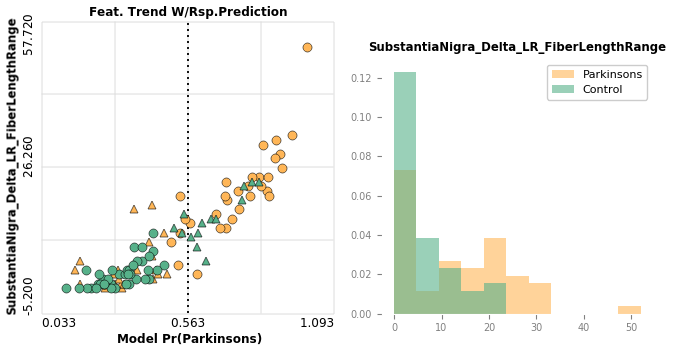
\includegraphics[width=0.9\textwidth]{DSFL.png}
% \caption{Comparing the distributions of the ``Delta-Left-Right Sum of Fiber Lengths" feature (absolute difference in sum of fiber lengths between the left and right hemispheres) between the control group (blue-green) and disease group (orange). Many more subjects from the disease group are within the higher range in the feature value, yet many disease group subjects have small differences from the control group.}
% \label{fig:DSFL}
% \end{figure}

% \begin{figure}[t]
% \centering
% 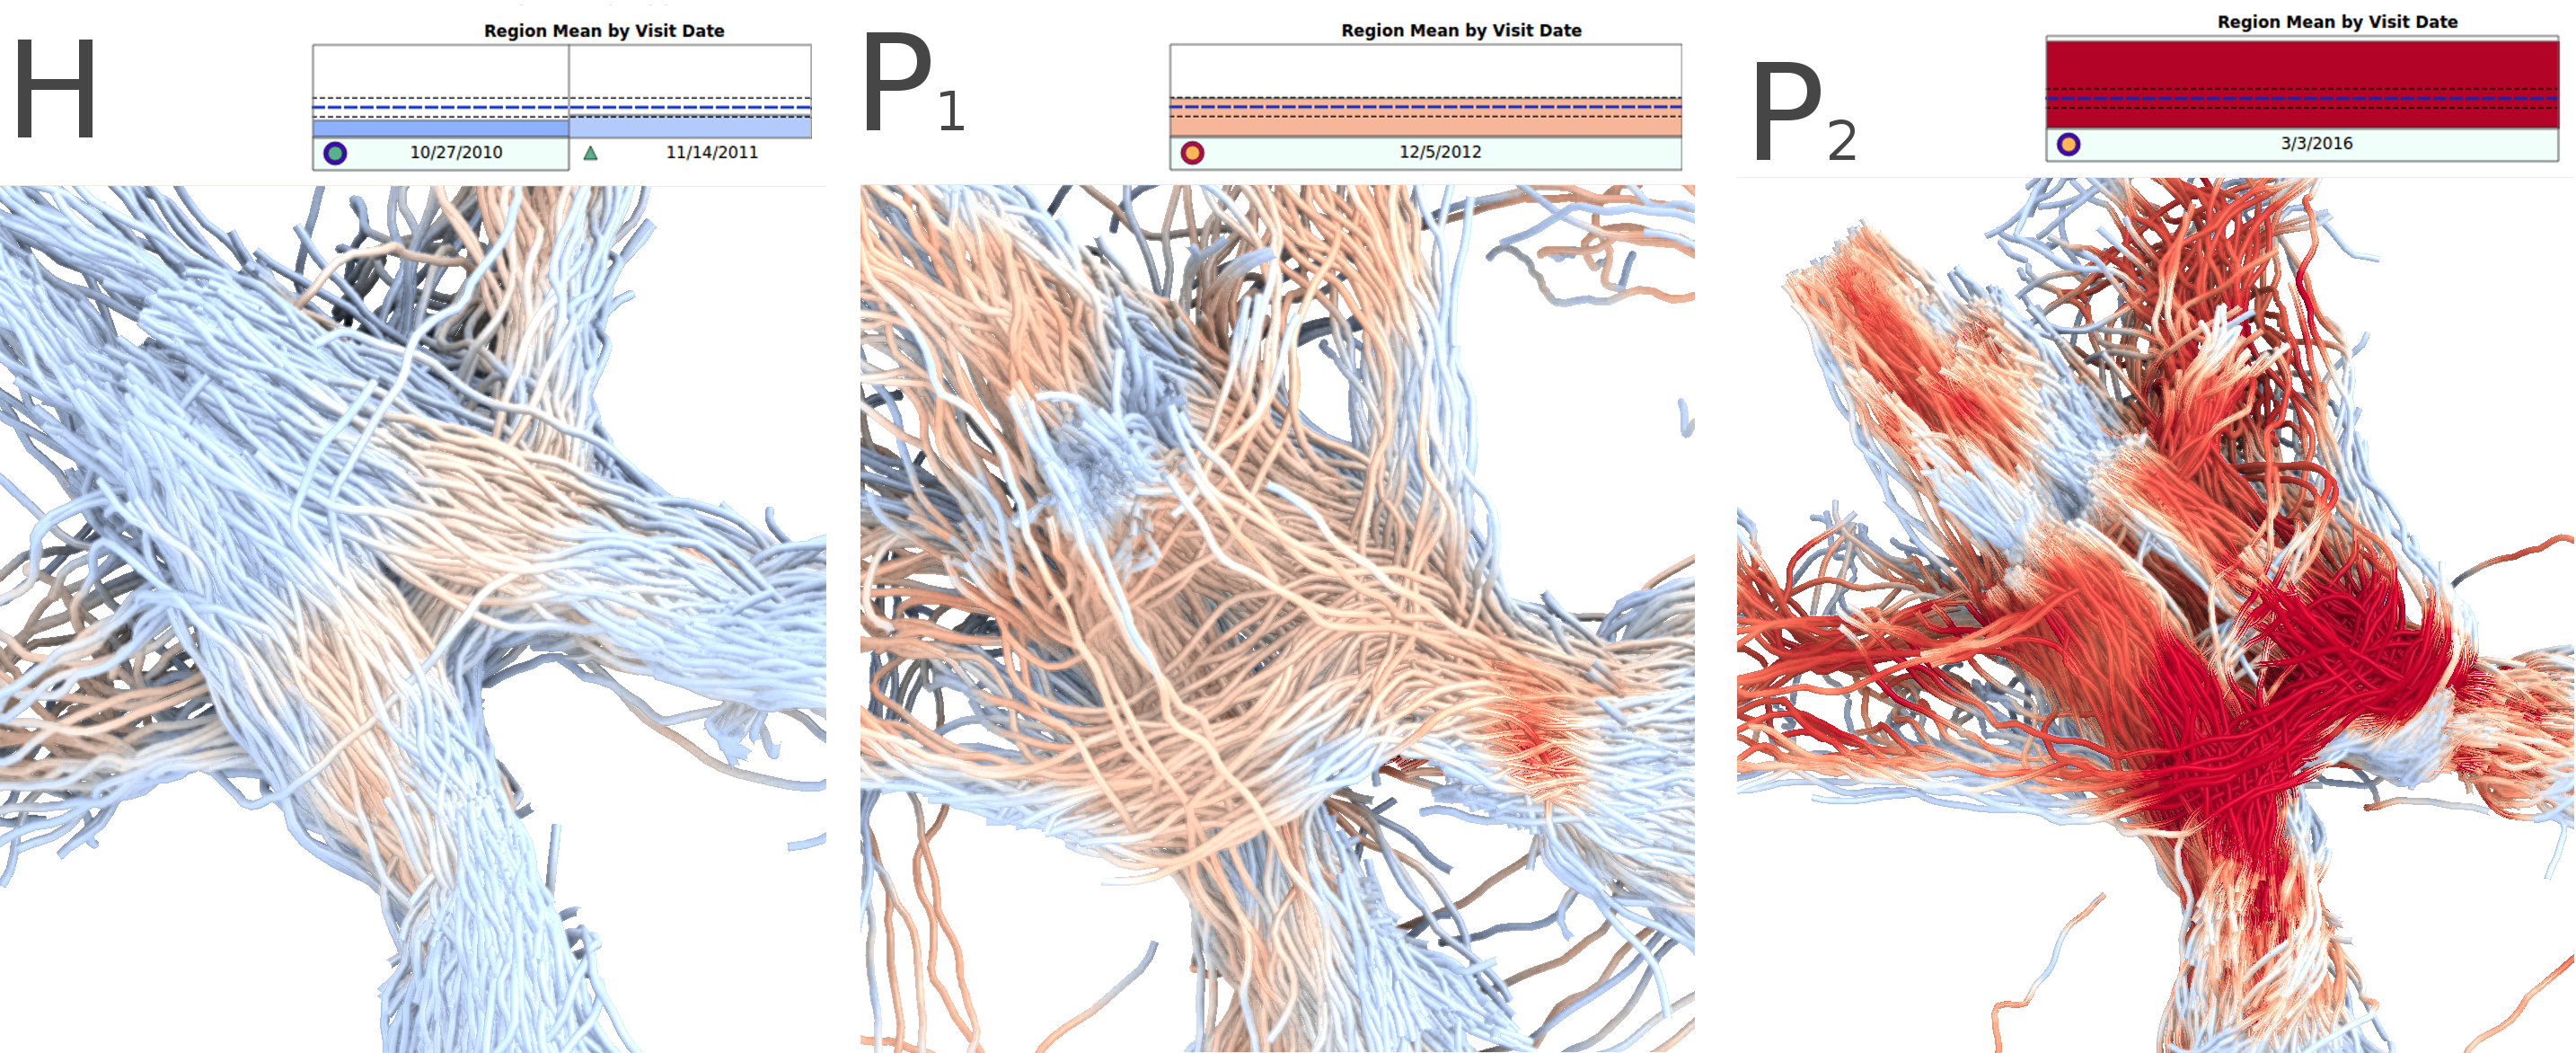
\includegraphics[width=0.9\textwidth]{SSO.png}
% \caption{The substantia nigra region is rendered with the S0 feature (raw T2 signal with no diffusion weighting) mapped using color. In the top $(H)$, the region is for a control subject that has overall lower values, and is without patches. This characteristic seemed more prevalent within the control group, yet many disease group subjects have this characteristic as well. The next two images $(P_1, P_2)$ each show brains fiber tracts from the disease group. In the middle $(P_1)$, patches of high values are observed in areas near the mid-section of the region. This characteristic seemed more prevalent in the disease group, yet is also found in many control group subjects as well. In the bottom ($P_2$), an example of a subject with abnormally high signal values throughout the mid-section and outer sections of the region. This effect seemed more prominent in more disease group subjects, yet was observed in some control group subjects as well.}
% \label{fig:SSO}
% \end{figure}


% \begin{figure}[t]
% \centering
% 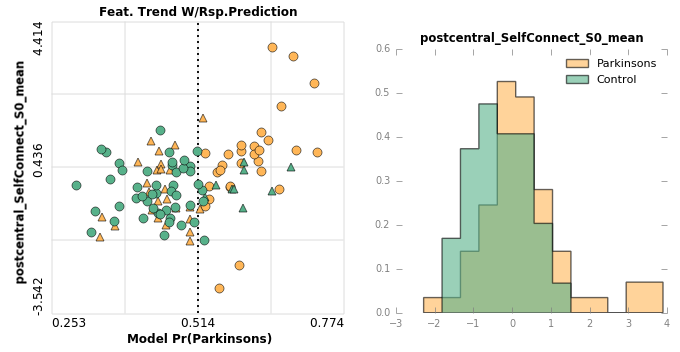
\includegraphics[width=0.9\textwidth]{PMSO.png}
% \caption{Comparing the distributions of the S0 feature (raw T2 signal with no diffusion weighting) between the control group (blue-green) and disease group (orange). The disease group's distribution is centering at a higher value than the control group and there are multiple outliers from the disease group in the high value range.}
% \label{fig:PMSO}
% \end{figure}


% \subsubsection{Analysis and Insights}

Based on the findings from previous works, we expected SN to be a high ranked region. However, with our data, we were only able to find noteworthy differences in older groups. As we seek to isolate smaller ranges of age, we run into problems where we don't have enough examples to make confident inferences. In addition, we find high variation in fiber features between individuals, making clear associations difficult. These problems can be addressed in further work using our system as data collections increase in size, and experts are able to refine the ROIs and feature engineering to better isolate the important differences.
% \textcolor{blue}{An expert suggests us to do \textit{t-test} on the two groups in the future, rather than visualize the distributions of the two groups, especially elderly male subjects. Since \textit{t-test} is a commonly used method in medical researches, the evaluated statistical difference of two groups may further help conduct a clinic meaningful indicators}.

% Due to the limited data size and the unbalanced data distribution, we initially split the data into 5 subgroups with a step size 20. Fig.~\ref{fig:groupDemographics} shows the demographics of the flatted 5 subgroups with balanced age and gender factors. In general, the prediction accuracy increase from 60\% to 90\% with age growth.

% Fig.~\ref{fig:SNcase} shows parts of our findings within the elderly group, with age from 70 to 90. Significant differences have been discovered that related to the AFL feature, one of the top scoring feature for the nigrostriatal fibers. Generally, as seen in the $Trend$ column, the AFL decreased in both HC and PD subjects at early ages. However, the HC group keeps the AFL steady, while in PD group it has a tendency of rapid decline. From the distribution of fiber length (the $DIST$ column), it is easy to find that the HC group overall has longer nigrostriatal fibers than the PD group. The third column image shows a typical HC group subject which has very complete nigrostriatal fibers, while the right 3 images show progressively worse cases of nigrostriatal fiber loss of a PD subject in different time steps. The coloring shows the difference in the length of the fiber from the average length of the control groups fibers for this region.

Beyond microstructural differences of the nigrostriatal tracts in PD subjects~\cite{zhang2015diffusion}, T2 hypointensity has been reported as a sensitive measure that is caused by iron accumulation in the substantia nigra in PD \cite{ollivier2018neuroimaging}. Lower S0 values may be a sign of higher iron concentrations~\cite{10.1001/archneur.59.1.62}. In our data, we found that overall the PD groups had lower mean value of S0 (MS0) in the SN region, though there are outliers with higher values. Though inconclusive, the gained insights might be useful for directing further research and for hypothesis generation. E3 pointed out that iron accumulation in one's brain may be caused by many different factors and the cause and pathogenesis of PD are not known nowadays; once observed, it is worth investigating how the iron has accumulated.

% Note that it is appears to be frequent in other ages. After mapping S0 feature to the fiber tracts, somehow we can see more red fibers in HC group subjects in the mid-section of the nigrostriatal fibers (near the center) at point level. 


% The S0 feature value of the PD group is lower than that of the HC group, which implies higher iron concentrations in PD subjects\cite{10.1001/archneur.59.1.62}. From the $DIST$ plot, the healthy subjects have higher S0 value on the whole than it in the PD group, though there are few outliers from the HC group in the high-value range. Note that it is appears to be frequent in other ages. After mapping S0 feature to the fiber tracts, somehow we can see more red fibers in HC group subjects in the mid-section of the nigrostriatal fibers (near the center) at point level. 



% there was still a lot of overlap between the disease and healthy control groups. By investigating the features of all age groups, we are able to see some interesting trends. The first is overall lower value, and less intense local values, which seems more typical of PD group fiber tracts. As seen in the distribution view of S0 feature in Fig.~\ref{fig:SNcase}, the S0 feature in the HC seems more concentrated and the value is higher on the whole, which is obvious among the subjects with age from 40 to 75. After detecting the features in the physical fiber rendering views with the values mapped to each point in each fiber, we were able to see the healthy subjects contains more red fiber tracts, which means lower S0 values and implies higher iron concentrations in Parkinson’s subjects\cite{10.1001/archneur.59.1.62}. However, it is not purely consistent across all age groups.  The distribution of S0 feature in youngest groups( age < 45 ) shows a contrary result that the disease group got higher S0 values than the HC. The second is the occurrences of patches of high S0 values occurring near the mid-section of the nigrostriatal fibers (near the center), as seen the red fibers in Fig.~\ref{fig:SNcase} and Fig.~\ref{fig:SNSteps}.  While this seemed more typical of the HC subjects, this effect was also noticed in some control group fiber tracts.

% After mapping it to nigrostriatal fiber tracts, we can see much of dark red that inflect higher water diffusion strength in the center of nigrostriatal fibers in Parkinson’s subjects, while those fibers are much lighter in healthy subjects.  The fiber tracts disappear from the dark red parts. This may be caused by the death of cells. 

% we expected to see nigrostriatal fiber loss.  and that the sum or average fiber lengths in the region would be good predictors. While we did see that average fiber length was a top scoring feature for the region, and that multiple Parkinson's subjects had high loss of fibers in the expected regions, these effects were not consistent across all of the subjects, and overall there is a large amount of overlap in the distributions of these features between the control and disease groups. One of the most significant features capturing the effect of fiber loss in the region seemed to be the absolute difference between the sum of the fiber lengths in the left hemisphere and right hemisphere (DSFL). Fig.~\ref{fig:DSFL} shows the distribution and scatter plot of the subjects average values over their predicted probabilities. Fig.~\ref{fig:loss} shows the type of loss we found in some of the Parkinson's brain fiber tracts in the SN region. The second column image shows a typical fully intact region for a control subject, while the right 3 images show progressively worse cases of fiber loss. The coloring shows the difference in the length of the fiber from the average length of the control groups fibers for this region.


% \subsubsection{Analysis 2: Raw T2 signal with no diffusion weighting (S0) of nigrostriatal DTI }

% One of the top ranked features for the nigrostriatal DTI was the raw T2 signal with no diffusion weighting (S0) feature, which may caused by iron accumulation in this nucleus. While ranked as one of best features, there was still a large overlap between the disease and healthy control groups, and the overall predictive power of the feature was still quite poor. By investigating the feature in the physical fiber rendering views with the values mapped to each point in each fiber, we were able to see some interesting trends and features. The trends that we found are shown in Fig.~\ref{fig:SSO}. The first is overall lower values, and less intense local values, which seems more typical of control group fiber tracts. The second is the occurrence of patches of high S0 values occurring near the mid-section of the nigrostriatal fibers (near the center), as seen the red spot in P1 image of Fig.~\ref{fig:SSO}. While this seemed more typical of the disease group subjects, this effect was also noticed in many control group fiber tracts. The last is characterized by very high intensities in the mid-section and mid-outer reaches of the fibers. This effect was noticed also in both groups, but seemed more typical of the PD. One interesting subject in particular is a 77 year old female with Parkinson's disease who has very complete nigrostriatal fibers. However, our classification models consistently predicted her to have Parkinson's with high confidence ($>90\%$ probability). After visualizing S0 mapped to the nigrostriatal fibers, we found she was an outlier in this feature with very high intensity values, likely this accounts for her high probability prediction.

% \begin{figure}[!ht]
% \centering
% 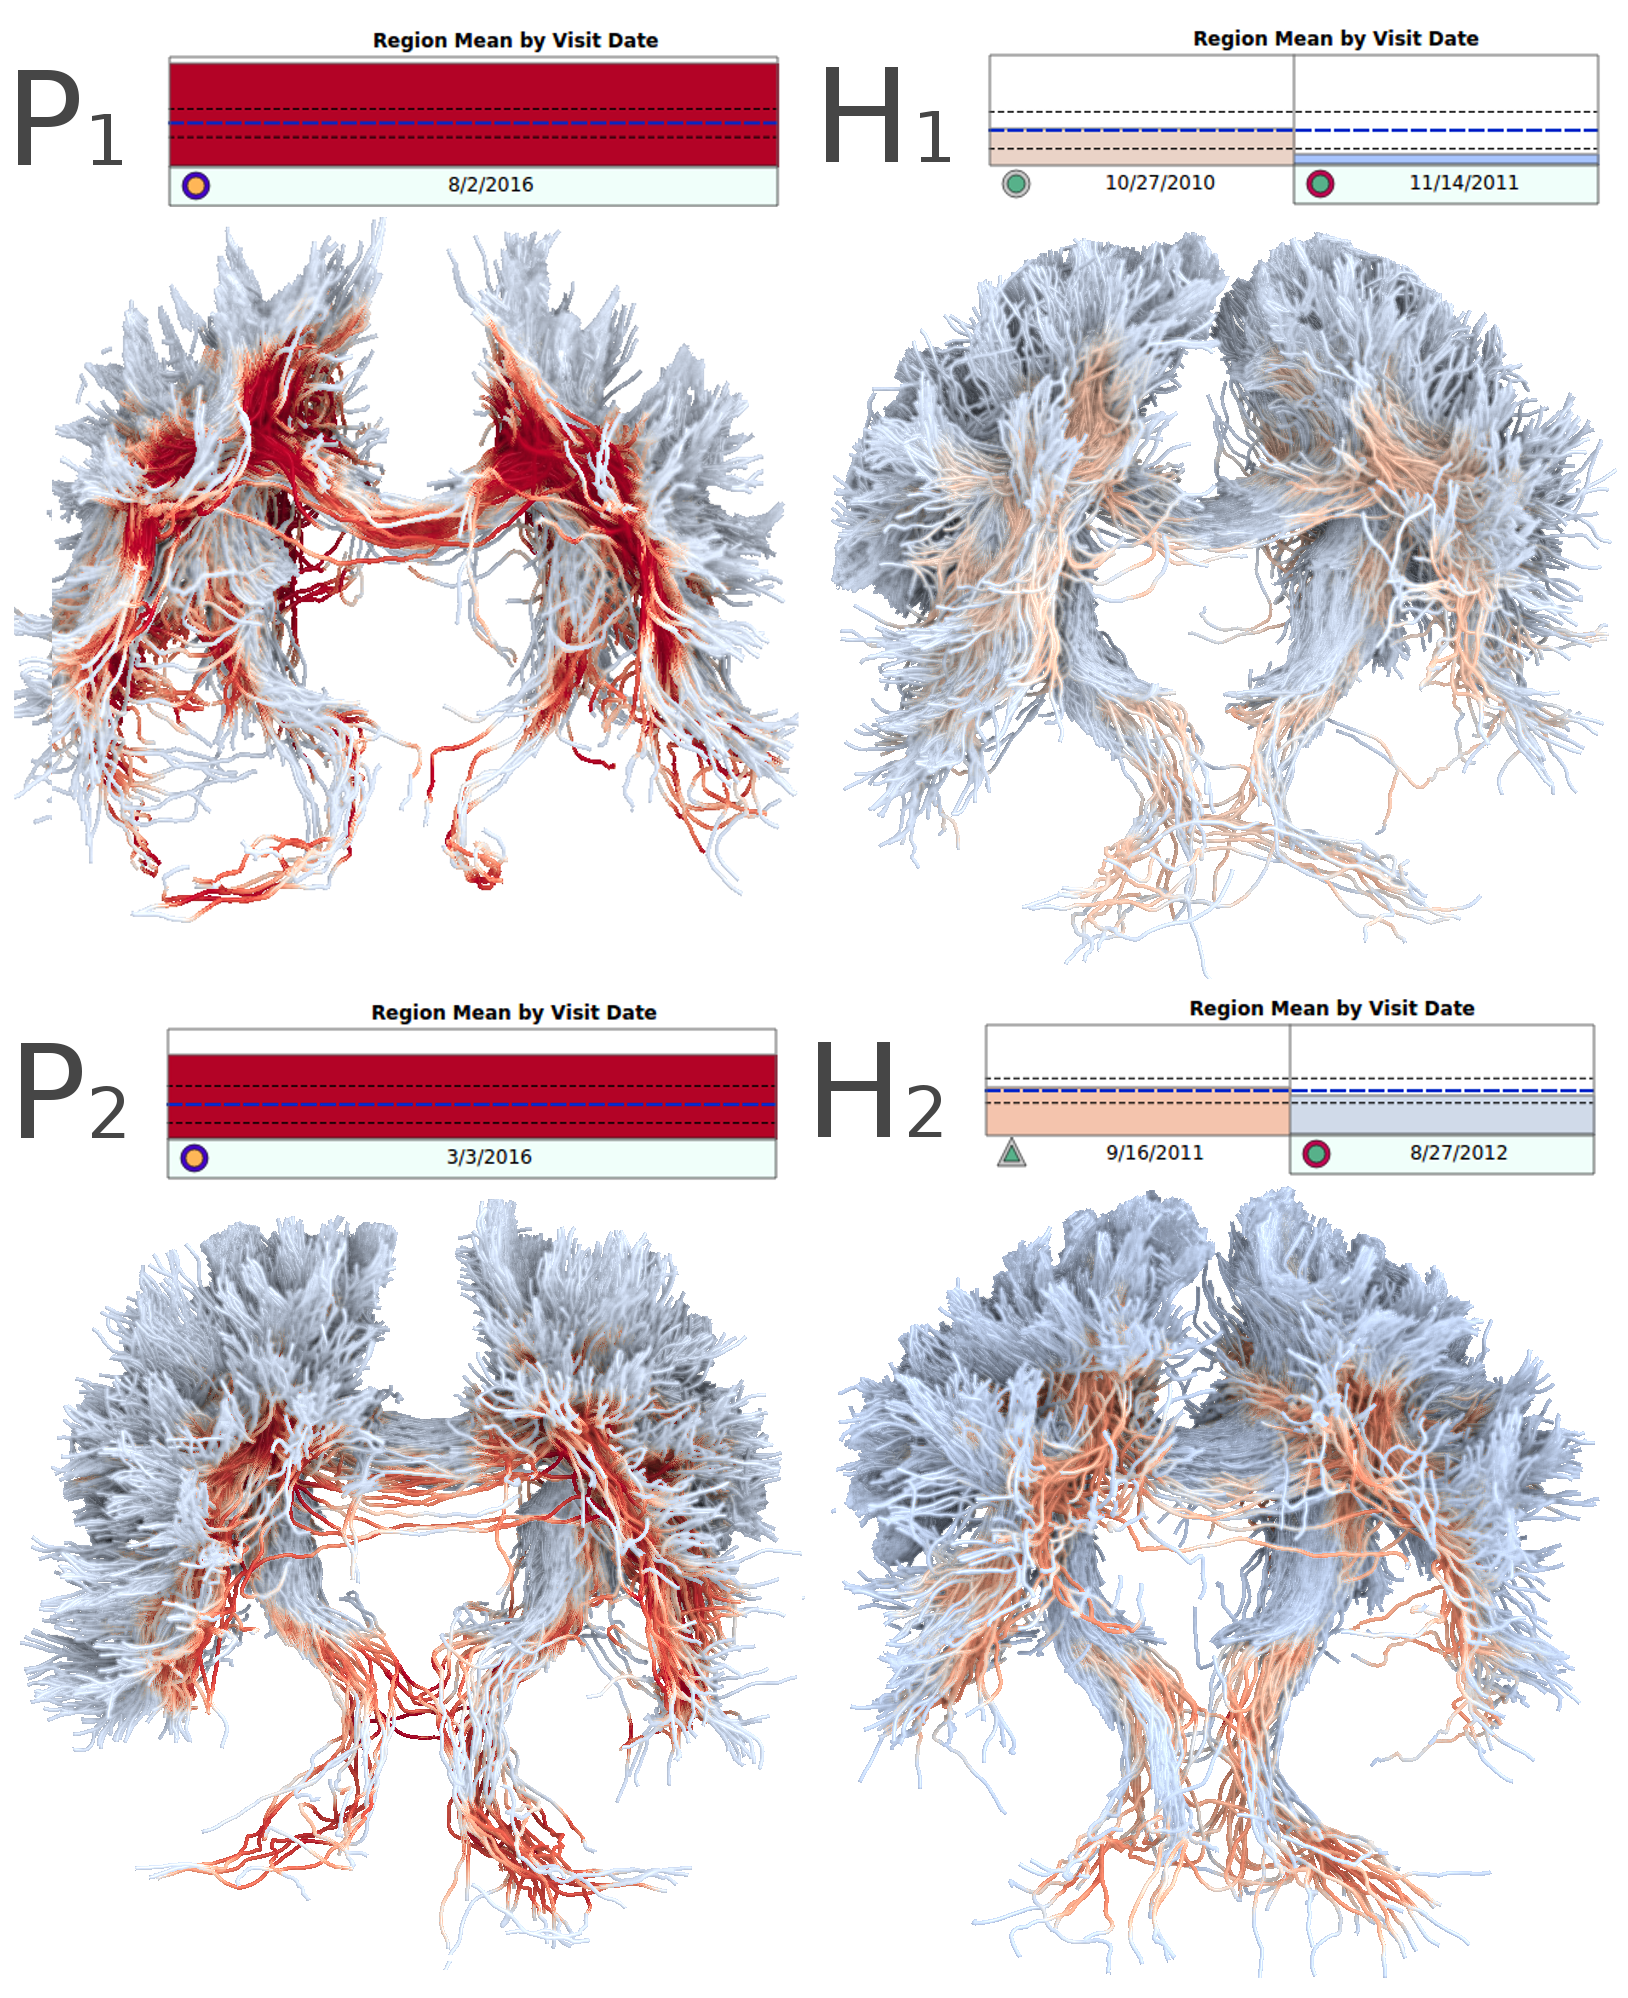
\includegraphics[width=0.9\textwidth]{pregion.png}
% \caption{Some examples mapping the Raw T2 signal with no diffusion weighting (S0) to the Post Central Region. On the left column we show two subjects from the disease group with a noticeable trend that we found to be mildly more prevalent in the disease group. On the right side we show two control group subjects for comparison.}
% \label{fig:pregion}
% \end{figure}

% \subsection{Case Study 2: Effects of Parkinson's on the Postcentral Region }

% In this case study, we gained an overview of the data and analyzed the data set without prior hypothesis. Based on the ML prediction results, we make new hypothesis that Postcentral region might has a strong influence on PD and investigated it through comparative visual analysis, which incorporating both information visualization and 3D rendering of the fiber tracts. 

% According to our system's forecast results, one of the top ranked region for prediction was the Postcentral region and the highest ranked feature within the region was the raw T2 signal with no diffusion weighting (S0). Based on those findings, we assume that the S0 feature in Postcentral region would have high probability of distinguishing between disease and non-disease. The distribution of the feature and scatter plot of all the subjects are shown in Fig.~\ref{fig:PMSO}. From the distribution view of the feature the mean value of S0 in PD is higher than the mean value of control group. In addition, the scatter plot shows the degree of discrimination between the two groups by using this feature. In order to explore the details in spatial space, the fiber tracts that passed through Postcentral region have been rendered in 3D space and the corresponding S0 features have been mapped to the fiber tracts based on their values. We investigated the feature values on the fibers in the physical space and found a trend similar to the trend we found for this feature in the SN region. Several images of the fiber rendering for this case are shown in Fig.~\ref{fig:pregion}. From the fiber rendering view, the fiber tracts of subjects are rendered deeper than those fiber of health. Similarly, from the timeline view, the mean values of S0 in disease subjects are much higher than the mean values of control group. Overall, it seems that the PD shows more subjects with higher values in the inner section of the region. 

% Though more detection about the disease on Postcentral region and S0 feature should be carried out and we are not able to verify how Postcentral region and S0 feature biologically affect PD, our system allows the researchers to have an overview of all the data and provides them with more hypothesis for further study. 



% \begin{figure*}[ht]
% \centering
% \includegraphics[width=1.0\textwidth]{images/fusiformCase.png}
% \caption{ Some examples mapping mean mode of the anisotropy (MMO) to the Fusiform Region. \circled{\small{a} and \circled{\small{b}} } show 3 subjects in different time steps from the PD group and HC group, with a noticeable trend that we found to be more red fiber tracts in the disease group, especially those fiber tracts on Inferior-Superior direction. \circled{\small{c} and \circled{\small{d}} } show MMO feature mapping to the whole brain fibers. There's a noticeable trend that the disease group subjects contain much more dark red spots and blue spots on the brain surface than those in control group.}
% \label{fig:fusiformCase}
% \end{figure*}


% \begin{figure*}[t]
% \centering
% 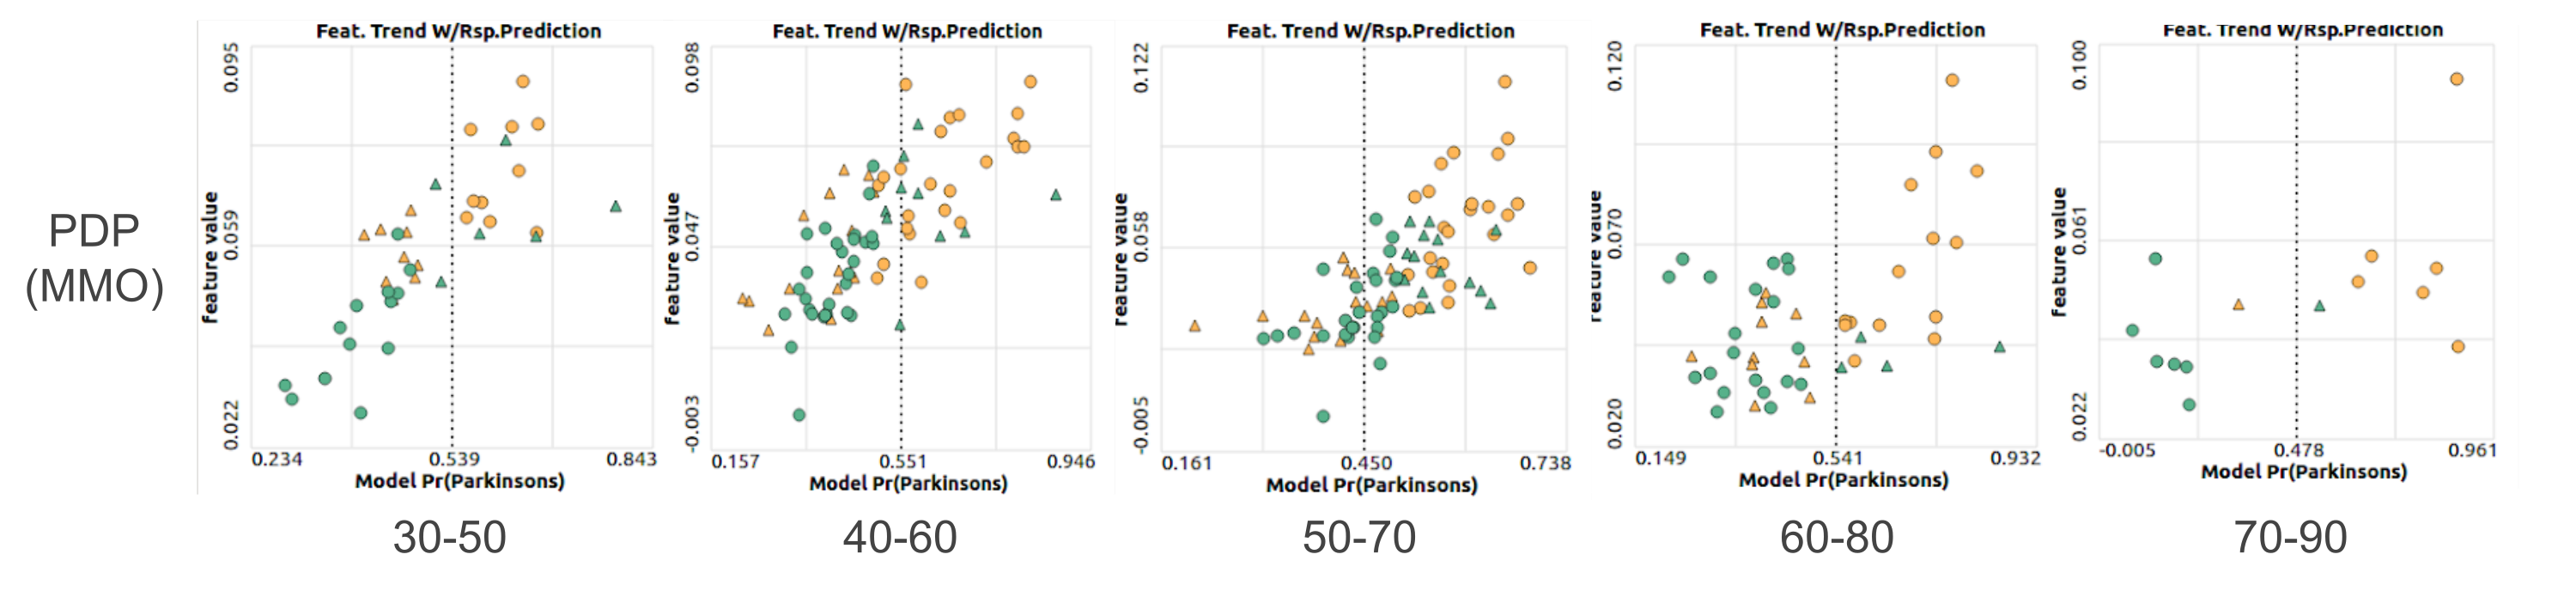
\includegraphics[width=0.85\textwidth]{images/PDP_MMO.png}
% \caption{Partial dependence plots of MMO feature in different ages. It shows strong correlation with PD in young ages}
% \label{fig:FG_PDP_MO}
% \end{figure*}


% \begin{figure}[t]
% \centering
% 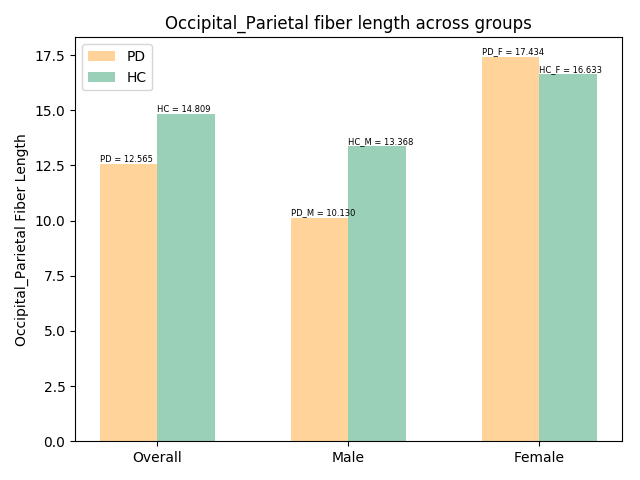
\includegraphics[width=0.95\textwidth]{images/Occipital_Parietal_Groups.png}
% \caption{ Average length of fibers connecting Occipital lobe and Parietal lobe. Overall, the fibers in HC group are longer than those in PD group, while female fiber length are longer than male's.}
% \label{fig:Occipital_Parietal_Groups}
% \end{figure}

% \begin{figure}[t]
% \centering
% 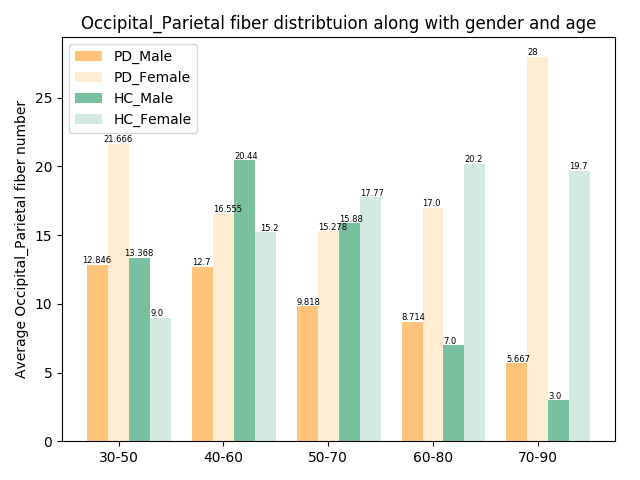
\includegraphics[width=0.95\textwidth]{images/Occipital_Parietal_gender_ages.png}
% \caption{ Average length of fibers connecting Occipital lobe and Parietal lobe. Overall, the fibers in HC group are longer than those in PD group, while female fiber length are longer than male's.}
% \label{fig:Occipital_Parietal_gender_ages}
% \end{figure}


% \begin{figure}[t]
% \centering
% 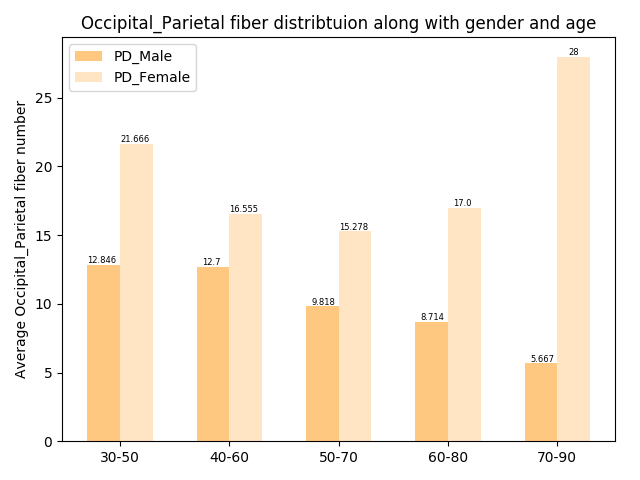
\includegraphics[width=0.95\textwidth]{images/Occipital_Parietal_gender_ages_PD.png}
% \caption{s.}
% \label{fig:Occipital_Parietal_AGE_PD}
% \end{figure}


% \begin{figure}[t]
% \centering
% 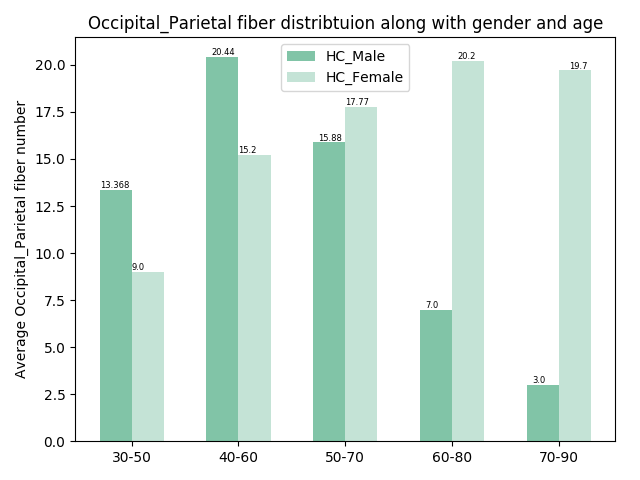
\includegraphics[width=0.95\textwidth]{images/Occipital_Parietal_gender_ages_HC.png}
% \caption{s.}
% \label{fig:Occipital_Parietal_AGE_HC}
% \end{figure}

% \subsection{Case Study 2: Exploration of Parkinson's Disease and the Fusiform Region}% (a hypothesis generation analysis)}

\subsection{Study 2: Exploration of PD with the Fusiform ROI}

% Additionally, we explored the fiber structure difference between HC and PD groups. Besides, age/gender-based exploration has been provided. Based on these analyses, we then provide new hypothesis which potentially would help in early oneset disease detection. 

\noindent In this study, we use our system with no assumptions to explore based on the estimated saliencies. We were interested in the following tasks: explore the brain regions that our system estimates to be the best predictors of PD, %based on our data, 
explore the top performing features in those salient regions, explore patterns of those features dis-aggregated and rendered in the physical space, and explore trends with age and gender.  

% We began by re-sampling our entire dataset without age restriction, and with stratification to balance our cohorts in class, age and gender (Fig.~\ref{fig:fusformSteps} \glf{A}). In total, we obtained 137 subjects, including 68 Parkinson's subjects and 69 healthy subjects. The demographics are shown in (\textbf{\textit{a2}}).

% While clicking the feature of interest in Fig.~\ref{fig:fusformSteps} \glf{C}, the information visualization views (Fig.~\ref{fig:fusformSteps} \glf{D}) show up without delay. After then, subjects are selected from the subjects performance table view (\textbf{\textit{c2}}) and the corresponding fiber tracts of this region are rendered side by side in the juxta-positioned 3D rendering views (Fig.~\ref{fig:fusformSteps} \glf{E}). 

We began by testing our system with the full set of subjects, including 68 PD subjects and 68 HC subjects. The balances in age and gender are shown in Fig.~\ref{fig:fusformSteps} \textbf{\textit{a2}}. After running the pipeline, our system estimated the fusiform ROI to be the best predictor by a small margin (Fig.\ref{fig:fusformSteps} \textbf{\textit{c1}}). The prediction accuracy is 70.1\% and $F_1$ is 0.701. The ROC curve helps show the variability of the classification performance, which gives insight into the uncertainty in the estimated region saliencies and subject prediction scores (Fig.~\ref{fig:fusformSteps} \glf{B}). The top performing feature within fusiform was mode of anisotropy (MO), which is a shape metric representing diffusion patterns (\textbf{\textit{c2}}). We noted that MO was also a top performing feature for many other regions, as well as the whole brain put together. The importance scrores for the 3 modalities of exploration are displayed in Fig.~\ref{fig:fusformSteps} \glf{C}. After selecting the fusiform region (\textbf{\textit{c1}}), we then select MO (\textbf{\textit{c2}}) and begin group and subject (\textbf{\textit{c3}}) level analysis. 

Group level analysis is done using several information visualization views. The parallel coordinates view (\textbf{\textit{d1}}) shows the trends of the top $K$ features. We can see that there is a high variation between subjects, and a lot of overlap in the distributions, while MO clearly shows the most notable differences. Plotting MO vs Pr(PD) (\textbf{\textit{d2}}) helps gain insight into the relationship between mean MO (MMO) to the classification model. An upward trend is noted, while the spread along the vertical axis suggests that other features are significantly taken into account for classification (motivating multivariate analysis). The covariance matrix view \textbf{\textit{d3}} is used to reveal relationships among the different features, and how those relationships differ between the groups. Fig.~\ref{fig:infovis} shows 2 example insights, while Fig.~\ref{fig:fusformSteps} \textbf{\textit{d3}} shows an additional example, where we see high covariance between f-SMS0 and f-MS0 (raw T2 signals in inter-connected and intra-connected fibers respectively). A basic group level comparison of MO is shown in the histogram view (Fig.~\ref{fig:infovis} \glf{D}). Additional comparisons with the fusiform region are shown in Fig.~\ref{fig:infovis}. 

After selecting two interesting subjects, the fibers are rendered in the 3D views and colored by MO. As we have found that the PD group has higher overall mean MO values, we inspect the dis-aggregated MO values as they are distributed on the fibers to look for patterns. For some HC subjects with low mean MO, we find a tendency to have a fuller set of fibers around the lower, outer egdes as can be seen in Fig.~\ref{fig:fusformSteps} \glf{E} and in another example Fig.~\ref{fig:infovis} \glf{E}. Those areas tend to also have lower MO values for both groups. Another common structural characteristic is that some subjects have fewer fibers connecting the occipital and parietal lobes; the ellipse parts in Fig.~\ref{fig:fusformSteps} \glf{E}. This is an interesting to feature to investigate further, since reduced fiber density connecting between the occipital and parietal lobes has been suggested to be a possible sign of diseased brain atrophy in PD~\cite{10.1093/brain/awh088}. 

Besides focusing on the fusiform, we also toggle between the whole brain colored by MO (Fig.~\ref{fig:fusformSteps} \glf{F}). While we notice higher values tend to be in the same areas for both groups, we notice some anomalies as shown in Fig.~\ref{fig:fusformSteps} \glf{E}, \glf{F}, where we discover large patches of high values (red) in a selected PD subject with high mean MO. These non-uniform higher intensity regions may be a factor in the predictive model, and we notice they tend to be found more in certain areas than others, which could inspire a further effort to localize and understand the cause. In the physiological sense, the different distributions of MO intensity indicate different patterns of water diffuse in different parts of the brain; however, imaging issues could also affect these tensor measures.

The insights we found, based on exploring in the physical space, is that it's not simply the case that the PD group has higher MO values, but rather that they may also have a different overall balance of fiber density in specific areas; those structural differences impact the average values since different areas tend to have higher or lower values in any case. This highlights that the impact of the tensor measure distributions in physical space is an important factor to consider (in relation to the average use for ML), and this factor is linked to structural differences between subjects as well. Since each brain is unique, both in relative local fiber density and in MO distribution, analysis of the feature can benefit greatly from inspecting in the physical space where these details can be observed, stressing the value of linked 3D visualization.  


In Fig.~\ref{fig:fusformSteps} \glf{G}, trends with age alone (\textbf{\textit{G1}}), and additionally with gender (\textbf{\textit{G2}}) are explored. Overall, the PD subjects have higher MO. However, as shown in \textbf{\textit{G2}}, the trend for the male and female subjects shows different patterns; on average, for the male subjects, MO decreased in age, while for females MO increased with age. However, the limited amount of data (especially in elderly female PD subjects) makes this insight highly uncertain; further investigation would be necessary. 

E2 showed interest in these case study findings. As mentioned by the experts, clinically, PD mainly has 5 symptoms: dementia, impaired balance, slowness (bradykinesia), stiffness (rigidity), and resting tremor. Each patient has one or more symptom, and each of the patient's symptoms are different. The loss of connection between the occipital and parietal lobes may be related to one symptom (e.g., impaired balance), while large patches in certain areas may be affiliated with other clinic symptoms. In addition, they suggested to co-analyze 
the MO feature with fiber loss. The MO feature may show a pattern when the impaired balance is not obvious in the early stage, but other patterns may emerge when impaired balance occurs.

% In addition, with selecting different time steps of a subject in the timeline views, we can have visual sense of the disease progress. Integrating brain region rendering, whole brain rendering and the subjects in different time steps, user would have a qualitative understanding of PD effects in physical space. Through empirical analysis, we discover more red spots and blue spots on the surface of the whole brain in the PD group than those in the HC group, especially in those subjects predicted true positive (TP) and true negative (TN). \textbf{(Task 1)}.  

% Back to the brain feature table view (\textbf{\textit{c3}}), the mean mode of the anisotropy ( MMO ) is a salient feature that is listed on the top of the table with low standard deviation. With clicking this feature, information visualization views of this feature would be shown in Fig.~\ref{fig:fusformSteps} \glf{D}. 

% Moreover, inspired by the performance of MMO in \textbf{\textit{d2}} and Fig.~\ref{fig:fusformSteps}  \glf{I}, we show our interest in the MMO feature effects at different ages. Splitting the dataset into $5$ subgroups as shown in Fig.~\ref{fig:groupDemographics}, we executed the ML pipeline multiple times with each subgroup subjects and obtained several partial dependence plots of MMO features at different ages (Fig.~\ref{fig:FG_PDP_MO}). Each subplot shows the relation between MMO feature and prediction outcome. The correlation between MMO and disease prediction is gradually weakening with age growth. In contrast to AFL of nigrostriatal fibers effects on PD in the previous case, it implies the MMO feature has a greater impact on the early PD. Since then, we may provide a hypothesis that MMO feature of one's brain might be relevant to the pathological characters of PD. Furthermore, it may potentially contribute to form a marker to identify early PD \textbf{(Task 3)}. 


% \subsubsection{Analysis and Insights}

% During the exploration process, we observe the disparity of fiber connection and the spots distribution difference between the HC group and the PD group. 


% The differences in MO intensity as they appear distributed on the fibers, indicates different patterns of how water molecules diffuse in different parts of the brain. We find it interesting, especially how the fiber structure, and relative density of fibers throughout the region can strongly have an impact on how the average, since there is also a strong correlation between region and MO intensity. 

% % More red spots and blue spots in PD brains may indicate a higher degree of water diffusion freedom. 

% Further analysis of such patterns may help neuroscients better understand how the disease spread in one's brain. Since these two manifestations appear to be more frequent incorrectly classified subjects than them in false predicted subjects, we suspect them contribute a lot to the model predictions.   

% According to the line charts of the MMO feature with respect to ages and genders, we find that PD is highly related to these two factors. \textbf{\textit{I1}} reveals that both the two groups have decline trends, but the value of MMO tends to be relatively higher in the PD group than it in the HC group. Moreover, with advancing age the MMO value overall has a decreasing tendency. This pattern could also be found in the male group in \textbf{\textit{I2}} (the solid lines). oppositely, the female group in \textbf{\textit{I2}} (the dotted lines) shows a relatively different pattern that have a promotion trend in elder ages. However, it may be biases that caused by the limited female subjects in the two groups, especially in the elder ages, as seen in Fig.~\ref{fig:groupDemographics}. Based on these findings, we could assume that the tendency in \textbf{\textit{I1}} is in a large part caused by males in \textbf{\textit{I2}}. Furthermore, we could make an assumption that men may be more likely to develop PD than women, which has been validated by researchers.\cite{Haaxma819}

 

 
%displays MMO value changes with advancing age and the MMO patterns on genders. We can clearly see different patterns in male and female groups, where male group shows decline trends with ages, but the female group seems to have a promotion trend in elder ages. However, it may be biases that caused by the limited female subjects in the two groups, especially in the elder ages, as seen in Fig.~\ref{fig:groupDemographics}

%For example, regarding the \textit{Air Force One } and \textit{Jumps} video (as shown in \autoref{case2_4}), the value of \textit{motion} score tends to be relatively higher, while the \textit{memory} and \textit{aesthetics} tend to be lower. This pattern could also be found in a bunch of videos of different types.
%However, the impact of such pattern varies among different video types, 




% Though many other fiber-tract based features like fiber number/ fiber length can differentiate PD group from HC, group , the current visual representation method, which just average the features and map them to fiber tracts, is still not good enough to show such features. The other tensor based features also show the capability to distinguish those two groups, it may not be obvious to see the features change when mapping them to the fiber tracts. MO feature in Fusiform region shows the changes both in physical structure as well as features distribution

% First, the fiber tracts go through the fusiform region. ( we call it single region fiber tracts ). Fig.~\ref{fig:fusiformCase} shows the fibers in PD group has more red fibers, which represent higher MO values have been mapped to the fiber tracts, than those in HC group. Even more, more fiber tracts on Inferior-Superior (I-S) direction, connecting from fusiform brain region and frontal lobe, especially caudal middle frontal and rostral middle frontal, have been found in PD group than those in HC group.   

% Second, from the whole brain fiber tracts, seen in Fig.~\ref{fig:fusformSteps} we can see much more and dark red spots or blue spots on the surface of the PD brains than in HC group brains. The brains with an extremely large amount of red surface are all in the TP group and FP group, where the healthy brains are predicted to be a diseased brain. While none brain that is characterized by an extremely large amount of red surface has been found in TN group and only one brain with such a trait in TN group has been FN group, where the disease brains are predicted to be a healthy brain.

% After exploring the data with our system, we can make a hypothesis that  the fiber tracts with darker red colors mapped to them on the brain surface in PD group might be affected by those red fibers connecting fusiform brain region and frontal lobe, where we can see the fiber tracts inside the dotted circle in Fig.~\ref{fig:fusformSteps}(E). Moreover, we make a hypothesis that those fibers might have a strong relationship with the disease. 

% Furthermore, we investigate which subjects contribute most to disease prediction and counting how much contribution to the predictions. Because we were using 5 folds cross-validation, we select the top N subjects, ranging from 6 to 30, from TP and TN groups. After running the ML pipeline multiple times, we got the accuracies of the top N subjects. From the accuracy curve in Fig.~\ref{fig:TopNaccPlot}, we observed that the classification accuracy goes to more than 85\% with top 16 subjects in each group, which implies those subjects contribute a lot to the predictions while using all the subjects in all ages. 

% To test those hypothesis, we perform a statistical analysis out of our system. we took all these brain fibers, from single region or whole brain, screenshots down and divided those screenshots into 4 groups, which are based on the prediction results ( TP, TN ,FP ,FN ) , respectively. Totally, we have 18 subjects in FP group, the minimum number of the 4 groups. We regard the top 18 brain with the highest prediction probability can be used to represent TN/TP group to a large extent. Here we consider top 18 brains in TP and TN groups, and top 18 brains in FP and FN groups. (Totally,  our dataset contains 68 HC subjects, in which 50 subjects in TN group and 18 subjects in FP group,  and 69 PD subjects, in which 45 subjects are in TP group and 24 subjects are in FN group ) 

% To test the first hypothesis, We perform a qualitative comparison, which is based on the red and blue spot coverage of the brain surface, in the 4 groups of the whole brain fibers. Fig.~\ref{fig:Fusiform_Spotcoverage} indicate the 

% We classify brains into 5 levels in visual perception. The more red on the brain surface, the lower the level is. Fig 20 shows the distributions of each group. It is easy to find the TP and FP groups have similar distributions, while the TN and FN groups have other distributions.

% In the 4 groups of the single region fibers, qualitative observation of the number of I-S fibers has been carried out. If the brain contains few fiber tracts, we mark it ``1'', conversely, we mark the brain as ``0''.  Then we come to the result, which is shown in Fig 21, that the HC and FN groups had a higher fiber reduction rate(  the ratio of ``1'' in the group ) than it in PD and FP groups. 

% Thence, our system supports  new  hypothesis generation  and  hypothesis-driven  analysis  of  the  disease. Moreover, our system can, to some extent, explain why the brain is predicted to be disease/healthy.

% \begin{figure}[t]
% \centering
% 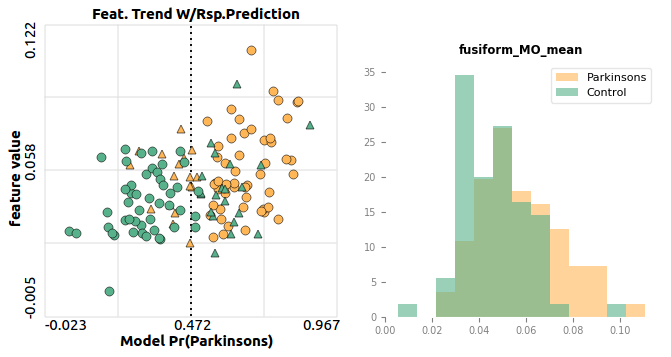
\includegraphics[width=0.9\textwidth]{images/Fusiform_MMO_distribution.png}
% \caption{Comparing the distributions of the MMO feature ( mean mode of the anisotropy ) between the control group (blue-green) and disease group (orange). The disease group’s distribution is centering at a higher value than the control group and there are few outliers from the health group in the high value range.}
% \label{fig:fusform_distribution}
% \end{figure}


% \begin{figure}[t]
% \centering
% 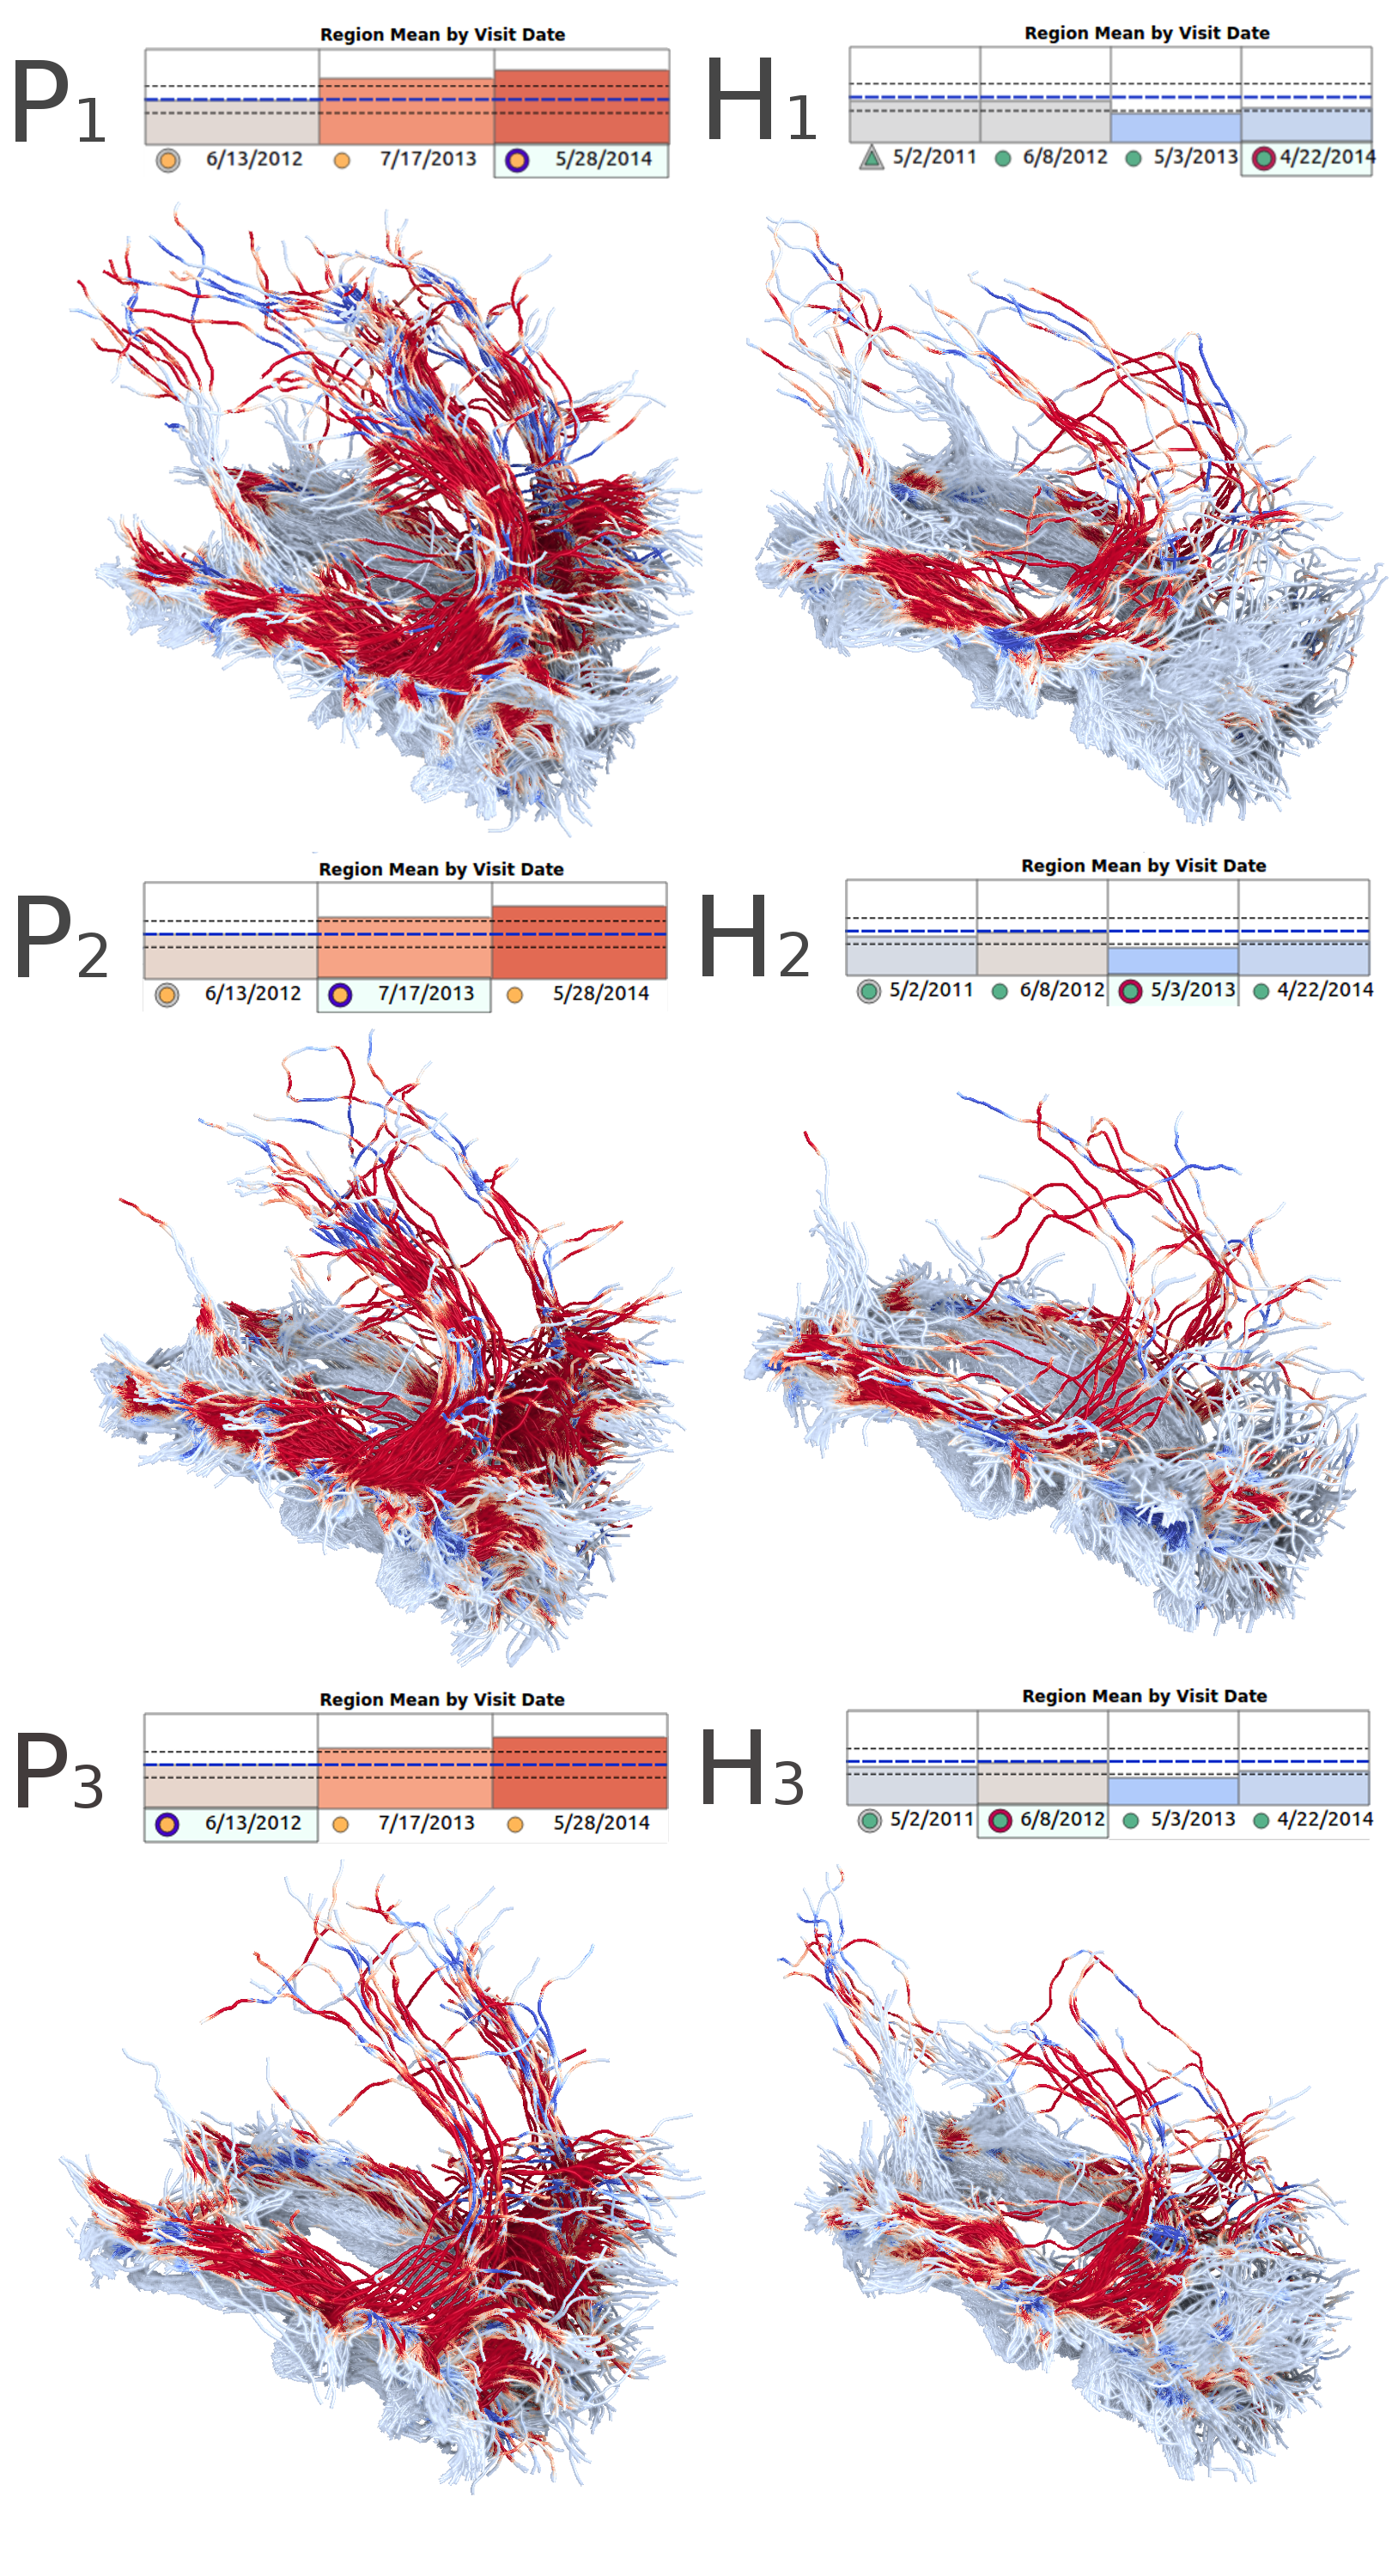
\includegraphics[width=1.0\textwidth]{images/Fusiform_MMO_Region.png}
% \caption{Some examples mapping mean mode of the anisotropy (MMO) to the Fusiform Region. On the left column we show 3 subjects in different time steps from the PD group with a noticeable trend that we found to be more red fiber tracts in the disease group, especially those fiber tracts on I-S direction. On the right side we show 3 control group subjects in different time steps for comparison. }
% \label{fig:fusform_region}
% \end{figure}

% \begin{figure}[!ht]
% \centering
% \includegraphics[width=1.0\textwidth]{images/fusiform_MMO.png}
% \caption{Some examples mapping the MMO feature to the whole brain fibers. The subjects are the same as that of the Fig.~\ref{fig:fusform_region}. There's a noticeable trend that the disease group subjects contain much more dark red spots or blue spots on the surface than those in control group. }
% \label{fig:fusform_surface}
% \end{figure}

% \begin{figure}[!ht]
% \centering
% 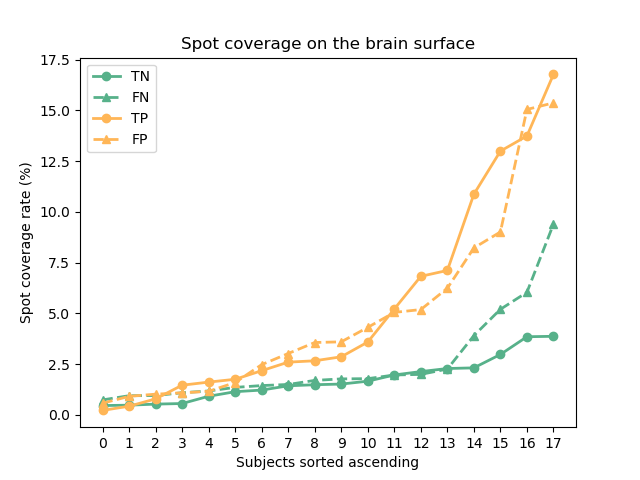
\includegraphics[width=0.9\textwidth]{images/Fusiform_Spotcoverage.png}
% \caption{.}
% \label{fig:Fusiform_Spotcoverage}
% \end{figure}
% \begin{figure}[!ht]
% \centering
% 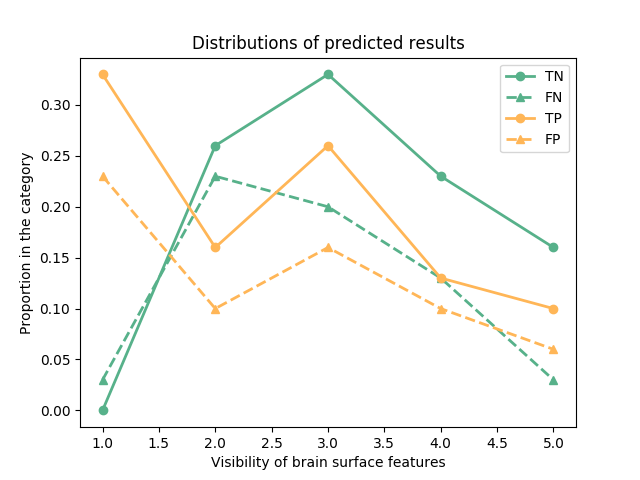
\includegraphics[width=0.9\textwidth]{images/Fusiform_BrainimageDistribution.png}
% \caption{.}
% \label{fig:Fusiform_BrainimageDistribution}
% \end{figure}

% \begin{figure}[!ht]
% \centering
% 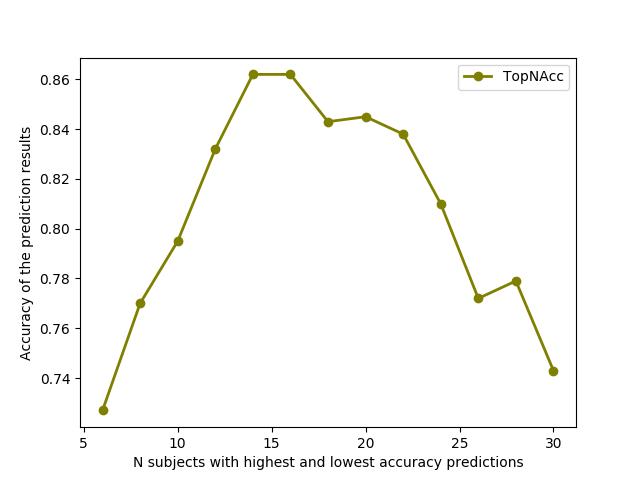
\includegraphics[width=0.9\textwidth]{images/TopNaccPlot.png}
% \caption{ Top $n$ subjects prediction accuracy. Selecting $n$ subjects from TP and TN groups, the prediction accuracy first increase then decrease with $n$ increase.}
% \label{fig:TopNaccPlot}
% \end{figure}

%\begin{figure}[!ht]
%\centering
%\includegraphics[width=0.9\textwidth]{images/fusiform_MO_distribution_wholebrain.png}
%\caption{we don't need it, just show how we get the figure 20}
%\label{fig:fusform_Mo_distribution_wholebrain}
%\end{figure}

%\begin{figure}[!ht]
%\centering
%\includegraphics[width=0.9\textwidth]{images/fusiform_MO_distribution_singleregion.png}
%\caption{we don't need it, just show how we get the figure 21}
%\label{fig:fusform_Mo_distribution_wholebrain_singleregion}
%\end{figure}

%On top of the fiber rendering view is the subjects information and their timeline showing their mean values of the selected feature against the control group mean for each of the subjects scans.

\vspace*{-0.06in}
\subsection{Expert Feedback}

\noindent Our team includes computer scientists with expertise in machine learning and visual analytics, and a computer scientist with some prior experience studying fiber tracts in an interdisciplinary lab. To help evaluate our work, we sought feedback from the experts.%2 domain experts (E4 and E5). , each with unique perspectives and backgrounds in neuroscience. The first (E1) is a neuroscientist with expertise in statistical analysis, tractography, and neurodenerative disease. The second (E2) is a neurologist at a children's hospital specializing in diagnosis and treatment of congenital nervous system malformations, and voxel-based morphometry (VBM) analysis of Huntington's disease.
%various congenital nervous system malformations, as well as brain trauma, tumors, and Huntington's disease.
%congenital nervous system malformations such as hydrocephalus, arachnoid cyst, tethered spinal chord, brain trauma, brain tumors, and Huntington's disease (a type of neurodenerative disease). 
We conducted live interactive demos to each of them, and also shared a draft of our manuscript. We then assimilated the feedback into our design and paper.

Several features were added based on these interactions. For example, E1 wanted to be able to investigate how age and gender affect the disease, so we modified the system so that it could further break down the data and visualize feature trends in these categories, as shown in Figure~\ref{fig:infovis} B. Also, while we originally used statistical significance testing as a feature ranking method, we changed our design to use Random Forest importance scores, as discussed in Section~\ref{sec:feature-sel}. Besides the advantages discussed already, part of the motivation for this is that significance testing can be easily misused and should be done under very careful experimental settings. The scores from Random Forest that we use, on the other hand, are not to be interpreted as anything more than a relative score that can be used for prioritized qualitative analysis, while the evidence of their relevance to the disease comes from the resulting performance of the classifier. However, one of the experts (E3) said they would still like to see \textit{p} values alongside the comparison of the distributions for added context. In the expert's field, the \textit{t-test} is commonly used, however it depends on the assumption of normality, which is not guaranteed to hold for all of the features in our data. Therefore, we instead chose to use the Mann-Whitney \textit{U-test}, which is a non-parametric statistical significance test that doesn't rely on the assumption of normality. According to the experts requests, the resulting \textit{p} values are shown for added context, however we emphasize the importance that the users interpret them carefully. Another issue that some of the experts had, was that they were distracted by the classification performance charts, which didn't need to be always visible. Therefore, we made these charts collapsible. Besides informing our design, E4 and E5 offered some big picture thoughts.

E4's assessment reflects an interest in DTI and fiber based bio-marker research. Since fiber based analysis of neurodenerative disease is still in the early stages, E4 said current research is highly exploratory. Advanced methods such as fiber tractography are emerging with promise for scientific discovery, however the complexity and uncertainty present daunting challenges which can be intimidating and "scare some researchers" away E4 said. In E4's experience: due to those complexities, and practical difficulty comparing many different individuals in the physical space, the focus tends to be more on statistical comparisons (e.g. DTI measures averaged in ROIs) than analysis of individual fiber tracts directly. For E4, physical analysis is usually initiated to investigate outliers. Overall, E4 thought that the system could make it more practical to do a qualitative analysis of the fibers more frequently. To E4, the concept of using AI to guide an exploratory VA process was new. E4 expressed concern that many neuroscientists don't have a background in ML, and that difficulty understanding ML models, parameters, and inputs, could be a discouraging factor. Since this is a novel area of research, the full impact that it will have is not completely understood. 

E5 thought the tool was innovative and useful as a research tool, but as a medical doctor was interested to envision how the work could eventually impact clinical practice. For research, the doctor said it could help in studying neurological disease from a new perspective. The expert believed that better understanding of changes in the fiber tracts could offer a new perspective into the morphological aspects of brain disease. However, in clinical practice, E5 expressed that only well understood and standardized markers can be translated into actionable insight. E5 also suggested that for clinical use a simplified system that hides the AI pipeline would be more usable, and that AI experts may need to be assigned to hospitals for them to properly utilize the technology. The doctor said that currently there are certain bio-markers that are very important in clinical practice for diagnosis and disease evaluation. It was suggested that a promising next step may be to analyze the co-occurrences of those markers with tract based features; in the long run, E5 suggested, those new features can be added as additional index variables in multi-modal disease severity grading systems. This could improve clinical practice by better defining and diagnosing disease characteristics, severity, and progression. While our system is designed for exploratory research, and the current scope is restricted to tract based analysis, we find these comments interesting and useful for VA researchers to plan future work. 
% Still, we note that our current system is able to incorporate other bio-markers into the ML pipeline and VA system so long as the data is available for each subject and can be input into the ML classification model. Besides enhancing prediction performance, and offering additional context and multi-modal insight, if the extra features also have a spatial component, they could be easily linked with the fiber tract ROIs. Still, there will be much room for future work specifically focusing on VA of multi-modal clinical characteristics. 
% As fiber-tract based research into neurodenerative disease matures, and findings are robustly validated, it may provide exciting and impact-full advancements with real world clinical applicability.

\subsection{Performance}
\label{sec:performance}
\noindent As mentioned in Sec.~\ref{sec:aggregation}, the user must wait for the machine learning pipeline to complete before the exploratory analysis. The time that this takes is highly dependent on data size and parameters in the ML pipeline. The most time intensive part of the pipeline comes from the extremely random trees/ensemble based feature importance algorithm that we use by default for feature saliency estimation. This comes with an option to choose the number of trees/estimators, which is linearly correlated with the run time; 150 is the default, but can go as high as 1500 to achieve moderately better results. CV parameters $k$ and $c$ are also linearly correlated with run-time. We tested the performance with a few reasonable settings, over all regions as described in Sec.~\ref{sec:aggregation},  with 136 subjects. The classifier we used was an SVM, and we used the default heuristic to train it on the top $\sqrt{n}$ ranked features (Sec.~\ref{sec:feature-sel}). The test machine had an Intel(R) Core(TM) i3-9100F CPU @ 3.60GHz. With the default parameters (150 estimators/trees, 5 CV folds, and $c=10$ repetitions of CV), the pipeline took 42 seconds. Increasing the number of estimators to 1500, and the CV folds to 10, it took 5 minutes and 25 seconds. These are reasonable wait times, since afterwards the user can explore without hesitation.
% \section{Performance}
% \label{sec:performance}

% {\color{red}Since performance may be brought up as an issue, and we now have space, it will be good to give some information about this.}

% %The connectome and fiber reconstruction process for each brain took us on average about $7$ hours, for a combined time of $~35$ days of processing on a medium powered desktop PC.

% For the interactive predictive analysis, the feature selection process completes in about $2$ seconds on average, while the group-wise subject classification time varies considerably depending on the model used. With the number of features and subjects we used, SVM, KNN, and Logistic Regression (the 3 highest performing models) were each able to be trained for each region and the full feature set, on average in less than $5$ seconds per cross-validation trial. This could be improved by training and testing the models for each region in parallel using separate python processes.
\section{Discussion and Limitations}

\noindent \textcolor{blue}{The ML apporaches that integrated in our system have been validated by the researchers in neuroscience~\cite{mateos2018structural,tanveer2020machine}. The features extracted from the DTI images also has been verified by research articles~\cite{acosta2016whole, wen2016white}.} Direct visualization of dis-aggregated features in the physical space can highlight underlying issues that affect the averages used for group level comparison. These patterns also have non-trivia physiological explanations that could enhance current understanding of neurodegenerative disease. As one gains insight into the important physical patterns, a rational next step would be to develop formalized descriptors that could be automatically extracted. While those important differences may be localized, precisely where they are localized, and how (or whether) they are expressed will vary between individuals. Currently, qualitative analysis through visualization is used to investigate those details, but it is a still a daunting task. Our tool will help to alleviate those difficulties, but significant challenges remain. One direction for further research is towards spatially invariant feature localisation and extraction using  neural networks (deep feature learning). As these kinds of advanced (often black box) methods are introduced, alleviating concerns about explain-ability, ease-of-use, and standardization are motivated; visualization can play a major role.

Another limitation comes from issues with data assimilation. Our current system requires the compared brain data to be obtained through identical imaging processes and also further be processed in a particular way afterwards. With more reliable techniques to assimilate data from different sources, it may be possible to greatly expand the amount of data that could be used together. With larger data, narrowing down significant differences would be easier, and more fine grained ROI/physical analysis as well as age and gender based analysis could be carried out with higher confidence. Since the state of the art in tractography is actively evolving, in the future there should be more standardized and well understood methods in use, which will appease researchers who wish to compare results between studies and maintain a comfortable understanding of the process to be confident in their judgements. 
It's noteworthy that 
current tractography can be computationally expensive. It took us about $60$ days in total to process about $190$ brain scans. Improved implementations better utilizing acceleration hardware such as GPUs will benefit the field tremendously. 



\section{Conclusions}

\noindent The system we introduce can effectively facilitate a deeper physical investigation into the statistical measures that are used by researchers to study differences between healthy control and neurodegenerative disease groups of DTI fiber tracts. The efficiency of the investigation is increased through intelligent guidance in the exploration process using predictive modelling, while comparative analysis is enhanced through customized interactive visualization views that are directly linked with each other and the predictive modelling pipeline. This set of views, with their encodings and interactions, help give better context to the observed differences, by simultaneously expressing multiple comparative modes for analysis and emphasizing uncertainty. This approach can benefit neurodegenerative disease researchers by helping them more easily gain a wide perspective into their data as they search for insights through an exploratory analysis process.

% further study 1: Though, our visual analytics system can help researchers discover some disease characteristics and deeper analyze the findings. A new methodology for automatically find the disease area and quantify the two subjects should be provided.



% To allow for easy dual compilation without having to reenter the
% abstract/keywords data, the \IEEEtitleabstractindextext text will
% not be used in maketitle, but will appear (i.e., to be "transported")
% here as \IEEEdisplaynontitleabstractindextext when the compsoc 
% or transmag modes are not selected <OR> if conference mode is selected 
% - because all conference papers position the abstract like regular
% papers do.
\IEEEdisplaynontitleabstractindextext
% \IEEEdisplaynontitleabstractindextext has no effect when using
% compsoc or transmag under a non-conference mode.



% For peer review papers, you can put extra information on the cover
% page as needed:
\ifCLASSOPTIONpeerreview
\begin{center} \bfseries EDICS Category: 3-BBND \end{center}
\fi
%
% For peerreview papers, this IEEEtran command inserts a page break and
% creates the second title. It will be ignored for other modes.
\IEEEpeerreviewmaketitle



% \IEEEraisesectionheading{\section{Introduction}\label{sec:introduction}}
% Computer Society journal (but not conference!) papers do something unusual
% with the very first section heading (almost always called "Introduction").
% They place it ABOVE the main text! IEEEtran.cls does not automatically do
% this for you, but you can achieve this effect with the provided
% \IEEEraisesectionheading{} command. Note the need to keep any \label that
% is to refer to the section immediately after \section in the above as
% \IEEEraisesectionheading puts \section within a raised box.




% The very first letter is a 2 line initial drop letter followed
% by the rest of the first word in caps (small caps for compsoc).
% 
% form to use if the first word consists of a single letter:
% \IEEEPARstart{A}{demo} file is ....
% 
% form to use if you need the single drop letter followed by
% normal text (unknown if ever used by the IEEE):
% \IEEEPARstart{A}{}demo file is ....
% 
% Some journals put the first two words in caps:
% \IEEEPARstart{T}{his demo} file is ....
% 
% Here we have the typical use of a "T" for an initial drop letter
% and "HIS" in caps to complete the first word.

% \IEEEPARstart{T}{his} demo file is intended to serve as a ``starter file''
% for IEEE Computer Society journal papers produced under \LaTeX\ using
% IEEEtran.cls version 1.8b and later.
% % You must have at least 2 lines in the paragraph with the drop letter
% % (should never be an issue)
% I wish you the best of success.
% \hfill mds
% \hfill August 26, 2015

% \subsection{Subsection Heading Here}
% Subsection text here.

% needed in second column of first page if using \IEEEpubid
%\IEEEpubidadjcol

% \subsubsection{Subsubsection Heading Here}
% Subsubsection text here.


% An example of a floating figure using the graphicx package.
% Note that \label must occur AFTER (or within) \caption.
% For figures, \caption should occur after the \includegraphics.
% Note that IEEEtran v1.7 and later has special internal code that
% is designed to preserve the operation of \label within \caption
% even when the captionsoff option is in effect. However, because
% of issues like this, it may be the safest practice to put all your
% \label just after \caption rather than within \caption{}.
%
% Reminder: the "draftcls" or "draftclsnofoot", not "draft", class
% option should be used if it is desired that the figures are to be
% displayed while in draft mode.
%
%\begin{figure}[!t]
%\centering
%\includegraphics[width=2.5in]{myfigure}
% where an .eps filename suffix will be assumed under latex, 
% and a .pdf suffix will be assumed for pdflatex; or what has been declared
% via \DeclareGraphicsExtensions.
%\caption{Simulation results for the network.}
%\label{fig_sim}
%\end{figure}

% Note that the IEEE typically puts floats only at the top, even when this
% results in a large percentage of a column being occupied by floats.
% However, the Computer Society has been known to put floats at the bottom.


% An example of a double column floating figure using two subfigures.
% (The subfig.sty package must be loaded for this to work.)
% The subfigure \label commands are set within each subfloat command,
% and the \label for the overall figure must come after \caption.
% \hfil is used as a separator to get equal spacing.
% Watch out that the combined width of all the subfigures on a 
% line do not exceed the text width or a line break will occur.
%
%\begin{figure*}[!t]
%\centering
%\subfloat[Case I]{\includegraphics[width=2.5in]{box}%
%\label{fig_first_case}}
%\hfil
%\subfloat[Case II]{\includegraphics[width=2.5in]{box}%
%\label{fig_second_case}}
%\caption{Simulation results for the network.}
%\label{fig_sim}
%\end{figure*}
%
% Note that often IEEE papers with subfigures do not employ subfigure
% captions (using the optional argument to \subfloat[]), but instead will
% reference/describe all of them (a), (b), etc., within the main caption.
% Be aware that for subfig.sty to generate the (a), (b), etc., subfigure
% labels, the optional argument to \subfloat must be present. If a
% subcaption is not desired, just leave its contents blank,
% e.g., \subfloat[].


% An example of a floating table. Note that, for IEEE style tables, the
% \caption command should come BEFORE the table and, given that table
% captions serve much like titles, are usually capitalized except for words
% such as a, an, and, as, at, but, by, for, in, nor, of, on, or, the, to
% and up, which are usually not capitalized unless they are the first or
% last word of the caption. Table text will default to \footnotesize as
% the IEEE normally uses this smaller font for tables.
% The \label must come after \caption as always.
%
%\begin{table}[!t]
%% increase table row spacing, adjust to taste
%\renewcommand{\arraystretch}{1.3}
% if using array.sty, it might be a good idea to tweak the value of
% \extrarowheight as needed to properly center the text within the cells
%\caption{An Example of a Table}
%\label{table_example}
%\centering
%% Some packages, such as MDW tools, offer better commands for making tables
%% than the plain LaTeX2e tabular which is used here.
%\begin{tabular}{|c||c|}
%\hline
%One & Two\\
%\hline
%Three & Four\\
%\hline
%\end{tabular}
%\end{table}


% Note that the IEEE does not put floats in the very first column
% - or typically anywhere on the first page for that matter. Also,
% in-text middle ("here") positioning is typically not used, but it
% is allowed and encouraged for Computer Society conferences (but
% not Computer Society journals). Most IEEE journals/conferences use
% top floats exclusively. 
% Note that, LaTeX2e, unlike IEEE journals/conferences, places
% footnotes above bottom floats. This can be corrected via the
% \fnbelowfloat command of the stfloats package.




% \section{Conclusion}
% The conclusion goes here.





% if have a single appendix:
%\appendix[Proof of the Zonklar Equations]
% or
%\appendix  % for no appendix heading
% do not use \section anymore after \appendix, only \section*
% is possibly needed

% use appendices with more than one appendix
% then use \section to start each appendix
% you must declare a \section before using any
% \subsection or using \label (\appendices by itself
% starts a section numbered zero.)
%


% \appendices
% \section{Proof of the First Zonklar Equation}
% Appendix one text goes here.

% % you can choose not to have a title for an appendix
% % if you want by leaving the argument blank
% \section{}
% Appendix two text goes here.


% use section* for acknowledgment
\ifCLASSOPTIONcompsoc
  % The Computer Society usually uses the plural form
  \section*{Acknowledgments}
%This research is sponsored in part by the U.S. National Science Foundation through grants IIS-528203 and IIS-1741536, the Nature Science Foundation of China through grant 61976075. We thank Dr. Pauline Maillard from Department of Neurology, University of California at Davis, Dr.Xiufang Xu from Hangzhou Medical College, and Dr.Chao Lin from Children's Hospital of Zhejiang University School of Medicine who provided insight and expertise that greatly assisted the research. We would also like to show our gratitude to Dr. Shunyuan Guo and Dr. Gaoping Lin from Zhejiang Provincial People’s Hospital for sharing their pearls of wisdom with us during this research.

Data used in the preparation of this article were obtained from the
Parkinson’s Progression Markers Initiative (PPMI) database (www.ppmiinfo.org/data). For up-to-date information on the study, visit www.ppmiinfo.org.
PPMI – a public-private partnership – is funded by the Michael J. Fox Foundation
for Parkinson’s Research and funding partners, including AbbVie, Allergan, Avid Radiopharmaceuticals, Biogen, BioLegend, Bristol-Myers Squibb, Celgene, Covance, GE Healthcare, Genentech, GlaxoSmithKline, Golub Capital, Handl Therapeutics, Insitro, Lilly, Lundbeck, Merck, MesoScaleDiscovery, Pfizer, Piramal, Prevail, Roche, Roche, SanofiGenzyme, Servier, Takeda, TEVA, UCB, Verily, and Voyager.
\else
  % regular IEEE prefers the singular form
  \section*{Acknowledgment}
\fi


% The authors would like to thank...


% Can use something like this to put references on a page
% by themselves when using endfloat and the captionsoff option.
\ifCLASSOPTIONcaptionsoff
  \newpage
\fi



% trigger a \newpage just before the given reference
% number - used to balance the columns on the last page
% adjust value as needed - may need to be readjusted if
% the document is modified later
%\IEEEtriggeratref{8}
% The "triggered" command can be changed if desired:
%\IEEEtriggercmd{\enlargethispage{-5in}}

% references section

% can use a bibliography generated by BibTeX as a .bbl file
% BibTeX documentation can be easily obtained at:
% http://mirror.ctan.org/biblio/bibtex/contrib/doc/
% The IEEEtran BibTeX style support page is at:
% http://www.michaelshell.org/tex/ieeetran/bibtex/
%\bibliographystyle{IEEEtran}
% argument is your BibTeX string definitions and bibliography database(s)
%\bibliography{IEEEabrv,../bib/paper}
%
% <OR> manually copy in the resultant .bbl file
% set second argument of \begin to the number of references
% (used to reserve space for the reference number labels box)
% \begin{thebibliography}{1}

% \bibitem{IEEEhowto:kopka}
% H.~Kopka and P.~W. Daly, \emph{A Guide to \LaTeX}, 3rd~ed.\hskip 1em plus
%   0.5em minus 0.4em\relax Harlow, England: Addison-Wesley, 1999.

% \end{thebibliography}

% biography section
% 
% If you have an EPS/PDF photo (graphicx package needed) extra braces are
% needed around the contents of the optional argument to biography to prevent
% the LaTeX parser from getting confused when it sees the complicated
% \includegraphics command within an optional argument. (You could create
% your own custom macro containing the \includegraphics command to make things
% simpler here.)
%\begin{IEEEbiography}[{\includegraphics[width=1in,height=1.25in,clip,keepaspectratio]{mshell}}]{Michael Shell}
% or if you just want to reserve a space for a photo:


\bibliographystyle{IEEEtran}
\bibliography{IEEEabrv,00_bibliography}


% \begin{IEEEbiography}{Michael Shell}
% Biography text here.
% \end{IEEEbiography}

% if you will not have a photo at all:
% \begin{IEEEbiographynophoto}{John Doe}
% Biography text here.
% \end{IEEEbiographynophoto}

% % insert where needed to balance the two columns on the last page with
% % biographies
% %\newpage

% \begin{IEEEbiographynophoto}{Jane Doe}
% Biography text here.
% \end{IEEEbiographynophoto}

% You can push biographies down or up by placing
% a \vfill before or after them. The appropriate
% use of \vfill depends on what kind of text is
% on the last page and whether or not the columns
% are being equalized.

%\vfill

% Can be used to pull up biographies so that the bottom of the last one
% is flush with the other column.
%\enlargethispage{-5in}



% that's all folks
\end{document}


